\documentclass[12pt]{book}

\usepackage{geometry} % Page layout
\usepackage{titlesec} % Formatting headings
\usepackage{fancyhdr} % Header/Footer
\usepackage{hyperref} % Hyperlinks
\usepackage{graphicx} % For images
\usepackage{amsmath} % For math
\usepackage{amssymb} % For math symbols
\usepackage{enumitem} % Custom lists
\usepackage[most]{tcolorbox}
\usepackage{epstopdf} % For converting EPS to PDF
\usepackage{pgfplots}
\usepackage{tikz}
\usepackage{float}
\usepackage{wrapfig}
\usepackage{svg}
\usepackage{draftwatermark}
\SetWatermarkText{Draft}
\SetWatermarkScale{4}
\SetWatermarkLightness{0.9}


\pgfplotsset{compat=1.18} % Important for log10

% Page layout
\geometry{a4paper, margin=1in}

% Header and footer
\pagestyle{fancy}
\fancyhf{}
\fancyhead[L]{Technical Ham}
\fancyhead[R]{}
\fancyfoot[C]{\thepage}

\titleformat{\chapter}[hang]{\huge\bfseries}{Chapter \thechapter}{1em}{}
\titleformat{\section}[hang]{\Large\bfseries}{\thesection}{0.5em}{}
\titleformat{\subsection}[hang]{\normalsize\bfseries}{\thesubsection}{1em}{}

\begin{document}

\tableofcontents
\newpage
\chapter{COMMISSION RULES}
\label{chapter:commission_rules}
\section{Introduction to the Amateur Radio Service}
\label{sec:intro_amateur_radio}

The Amateur Radio Service, often referred to as ham radio, is a popular hobby and service that brings people, electronics, and communication together. It is a unique blend of technical skill, public service, and international camaraderie. This section introduces the fundamental concepts of the Amateur Radio Service, including its purpose, regulatory framework, and key definitions.

\subsection*{Basis and Purpose of the Amateur Radio Service}
The Amateur Radio Service is governed by a set of principles and purposes that guide its operation. According to the Federal Communications Commission (FCC), the primary purpose of the Amateur Radio Service is to advance skills in the technical and communication phases of the radio art. This includes fostering experimentation, improving technical proficiency, and providing a pool of trained operators who can assist in times of emergency. The service also promotes international goodwill by allowing operators to communicate across borders.

\subsection*{Regulatory Authority of the FCC}
The FCC is the primary regulatory body responsible for overseeing the Amateur Radio Service in the United States. The FCC establishes and enforces the rules that govern amateur radio operations, ensuring that the service operates in the public interest. These rules are codified in Title 47 of the Code of Federal Regulations, Part 97 (FCC Part 97). The FCC also maintains the Universal Licensing System (ULS), a database that contains information about all licensed amateur radio operators and stations.

\begin{figure}[ht]
    \centering
    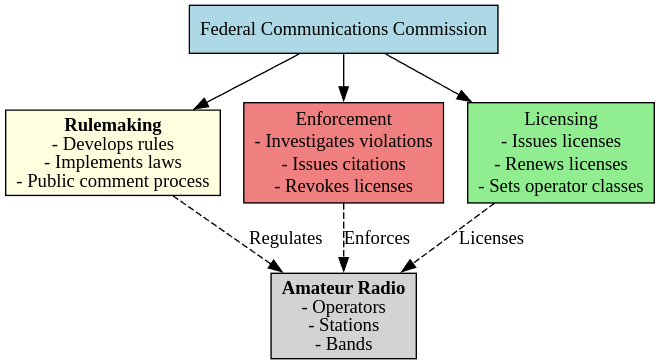
\includegraphics[width=0.8\textwidth]{tech/organized/chapter_1/images/fcc_structure.png}
    \caption{FCC Regulatory Structure}
    \label{fig:fcc_structure}
    % Diagram showing the structure of the FCC and its role in amateur radio regulation. The diagram should include the FCC at the top, with branches for rulemaking, enforcement, and licensing. Arrows should indicate the flow of authority and responsibility.
\end{figure}


\subsection*{Phonetic Alphabet Usage}
The use of a phonetic alphabet is encouraged in the Amateur Radio Service, particularly for station identification. The phonetic alphabet helps to ensure clarity and accuracy in communication, especially when dealing with weak signals or noisy conditions. While not mandatory in all situations, its use is a best practice that enhances the effectiveness of amateur radio communications.

\begin{table}[ht]
    \centering
    \begin{tabular}{|l|l||l|l||l|l|}
        \hline
        A & Alpha & J & Juliet & S & Sierra \\
        B & Bravo & K & Kilo & T & Tango \\
        C & Charlie & L & Lima & U & Uniform \\
        D & Delta & M & Mike & V & Victor \\
        E & Echo & N & November & W & Whiskey \\
        F & Foxtrot & O & Oscar & X & X-ray \\
        G & Golf & P & Papa & Y & Yankee \\
        H & Hotel & Q & Quebec & Z & Zulu \\
        I & India & R & Romeo & & \\
        \hline
    \end{tabular}
    \caption{NATO Phonetic Alphabet}
    \label{tab:phonetic_alphabet}
\end{table}

\subsection*{License Grants and Documentation}
An individual may hold only one operator/primary station license grant at any given time. This license is documented in the FCC ULS database, which serves as the official record of the license grant. The appearance of the license in the ULS database is the definitive proof that the FCC has issued the license. Printed copies or email notifications are not considered official documentation.

\subsection*{Definitions of Beacon and Space Station}
FCC Part 97 provides specific definitions for key terms used in the Amateur Radio Service. A \textit{beacon} is defined as an amateur station that transmits communications for the purposes of observing propagation or related experimental activities. A \textit{space station}, on the other hand, is an amateur station located more than 50 km above Earth's surface. These definitions are important for understanding the scope and limitations of amateur radio operations.

\subsection*{Questions}

\begin{tcolorbox}[colback=gray!10!white,colframe=black!75!black,title={T1A01}]
    Which of the following is part of the Basis and Purpose of the Amateur Radio Service?
    \begin{enumerate}[label=\Alph*),noitemsep]
        \item Providing personal radio communications for as many citizens as possible
        \item Providing communications for international non-profit organizations
        \item \textbf{Advancing skills in the technical and communication phases of the radio art}
        \item All these choices are correct
    \end{enumerate}
\end{tcolorbox}
The Basis and Purpose of the Amateur Radio Service, as defined by the FCC, includes advancing skills in the technical and communication phases of the radio art. This is the primary goal of the service, making option C correct. Options A and B are not part of the official basis and purpose.

%memory_trick T1A01

\begin{tcolorbox}[colback=gray!10!white,colframe=black!75!black,title={T1A02}]
    Which agency regulates and enforces the rules for the Amateur Radio Service in the United States?
    \begin{enumerate}[label=\Alph*),noitemsep]
        \item FEMA
        \item Homeland Security
        \item \textbf{The FCC}
        \item All these choices are correct
    \end{enumerate}
\end{tcolorbox}
The Federal Communications Commission (FCC) is the agency responsible for regulating and enforcing the rules for the Amateur Radio Service in the United States. This is clearly stated in FCC Part 97.

%memory_trick T1A02

\begin{tcolorbox}[colback=gray!10!white,colframe=black!75!black,title={T1A03}]
    What do the FCC rules state regarding the use of a phonetic alphabet for station identification in the Amateur Radio Service?
    \begin{enumerate}[label=\Alph*),noitemsep]
        \item It is required when transmitting emergency messages
        \item \textbf{It is encouraged}
        \item It is required when in contact with foreign stations
        \item All these choices are correct
    \end{enumerate}
\end{tcolorbox}
The FCC encourages the use of a phonetic alphabet for station identification, but it is not mandatory in all situations. This practice helps to ensure clear communication, especially under challenging conditions.

%memory_trick T1A03

\begin{tcolorbox}[colback=gray!10!white,colframe=black!75!black,title={T1A04}]
    How many operator/primary station license grants may be held by any one person?
    \begin{enumerate}[label=\Alph*),noitemsep]
        \item \textbf{One}
        \item No more than two
        \item One for each band on which the person plans to operate
        \item One for each permanent station location from which the person plans to operate
    \end{enumerate}
\end{tcolorbox}
An individual may hold only one operator/primary station license grant at any given time. This is a fundamental rule in the Amateur Radio Service.

%memory_trick T1A04

\begin{tcolorbox}[colback=gray!10!white,colframe=black!75!black,title={T1A05}]
    What proves that the FCC has issued an operator/primary license grant?
    \begin{enumerate}[label=\Alph*),noitemsep]
        \item A printed copy of the certificate of successful completion of examination
        \item An email notification from the NCVEC granting the license
        \item \textbf{The license appears in the FCC ULS database}
        \item All these choices are correct
    \end{enumerate}
\end{tcolorbox}
The official proof of an operator/primary license grant is its appearance in the FCC ULS database. Printed copies or email notifications are not considered official documentation.

%memory_trick T1A05

\begin{tcolorbox}[colback=gray!10!white,colframe=black!75!black,title={T1A06}]
    What is the FCC Part 97 definition of a beacon?
    \begin{enumerate}[label=\Alph*),noitemsep]
        \item A government transmitter marking the amateur radio band edges
        \item A bulletin sent by the FCC to announce a national emergency
        \item A continuous transmission of weather information authorized in the amateur bands by the National Weather Service
        \item \textbf{An amateur station transmitting communications for the purposes of observing propagation or related experimental activities}
    \end{enumerate}
\end{tcolorbox}
A beacon, as defined by FCC Part 97, is an amateur station that transmits communications for the purposes of observing propagation or related experimental activities. This definition is specific to the Amateur Radio Service.

%memory_trick T1A06

\begin{tcolorbox}[colback=gray!10!white,colframe=black!75!black,title={T1A07}]
    What is the FCC Part 97 definition of a space station?
    \begin{enumerate}[label=\Alph*),noitemsep]
        \item Any satellite orbiting Earth
        \item A manned satellite orbiting Earth
        \item \textbf{An amateur station located more than 50 km above Earth's surface}
        \item An amateur station using amateur radio satellites for relay of signals
    \end{enumerate}
\end{tcolorbox}
A space station, according to FCC Part 97, is an amateur station located more than 50 km above Earth's surface. This definition distinguishes space stations from other types of amateur stations.

%memory_trick T1A07

\subsection*{Summary}
This section introduced the Amateur Radio Service, its purpose, and the regulatory framework established by the FCC. Key concepts include:

\begin{itemize}
    \item \textbf{Purpose of the Amateur Radio Service}: Advancing technical and communication skills, fostering experimentation, and providing emergency communications.
    \item \textbf{Regulatory authority of the FCC}: The FCC regulates and enforces the rules for amateur radio operations in the United States.
    \item \textbf{Phonetic alphabet usage}: Encouraged for clear and accurate station identification.
    \item \textbf{License grants and documentation}: Only one operator/primary station license grant is allowed per person, and the license must appear in the FCC ULS database.
    \item \textbf{Definitions of beacon and space station}: A beacon is an amateur station for propagation observation, while a space station is located more than 50 km above Earth's surface.
\end{itemize}

\section{Frequency Coordination and Band Usage}
\label{sec:frequency_coordination}

\subsection*{Role of Frequency Coordinators}
Volunteer frequency coordinators play a crucial role in managing the allocation of transmit/receive channels and other parameters for auxiliary and repeater stations. These coordinators are recognized by local amateur operators and are responsible for ensuring efficient use of the frequency spectrum. They are selected by amateur operators in a local or regional area whose stations are eligible to be repeater or auxiliary stations. This decentralized approach allows for flexibility and adaptability to local needs.

\subsection*{Frequency Ranges for Technician Licensees}
Technician class licensees have access to specific frequency ranges for phone operation. These include the 28.300 MHz to 28.500 MHz segment of the 10-meter band. This range is particularly useful for voice communication and is a key privilege for Technician licensees.

\subsection*{International Space Station (ISS) Communication}
Amateur radio operators holding a Technician class or higher license are permitted to contact the International Space Station (ISS) on VHF bands. This privilege allows for direct communication with astronauts and participation in educational outreach programs.

\subsection*{Amateur Band Segments and Their Usage}
Amateur radio bands are divided into segments, each with specific uses and operating privileges. Technician class operators have access to various frequency bands, with different permitted modes of operation in each segment.

\begin{table}[h]
    \centering
    \begin{tabular}{|l|l|l|l|}
        \hline
        \textbf{Band Name} & \textbf{Frequency Range} & \textbf{Modes Permitted} & \textbf{Notes} \\
        \hline
        10 Meters & 28.000-28.300 MHz & CW, RTTY, Data & \\
        & 28.300-28.500 MHz & Phone, CW & Voice privileges \\
        \hline
        6 Meters & 50.0-54.0 MHz & CW, Phone, Image, & Including 52.525 MHz \\
        & & RTTY, Data & calling frequency \\
        \hline
        2 Meters & 144.0-148.0 MHz & CW, Phone, Image, & Including 146.52 MHz \\
        & & RTTY, Data & calling frequency \\
        \hline
        1.25 Meters & 219-220 MHz & Digital messaging & Fixed digital forwarding \\
        & & systems only & systems only \\
        & 222-225 MHz & CW, Phone, Image, & \\
        & & RTTY, Data & \\
        \hline
        70 Centimeters & 420-450 MHz & CW, Phone, Image, & \\
        & & RTTY, Data & \\
        \hline
        33 Centimeters & 902-928 MHz & CW, Phone, Image, & \\
        & & RTTY, Data & \\
        \hline
        23 Centimeters & 1240-1300 MHz & CW, Phone, Image, & \\
        & & RTTY, Data & \\
        \hline
        \multicolumn{4}{|l|}{Additional bands above 2.3 GHz also available to Technicians} \\
        \hline
    \end{tabular}
    \caption{Technician License Frequency Privileges and Operating Modes}
    \label{tab:technician_privileges}
\end{table}

\subsection*{Questions}
\begin{tcolorbox}[colback=gray!10!white,colframe=black!75!black,title={T1A08}]
    Which of the following entities recommends transmit/receive channels and other parameters for auxiliary and repeater stations?
    \begin{enumerate}[label=\Alph*),noitemsep]
        \item Frequency Spectrum Manager appointed by the FCC
        \item \textbf{Volunteer Frequency Coordinator recognized by local amateurs}
        \item FCC Regional Field Office
        \item International Telecommunication Union
    \end{enumerate}
\end{tcolorbox}
Volunteer frequency coordinators are recognized by local amateur operators and are responsible for recommending transmit/receive channels and other parameters for auxiliary and repeater stations. The FCC does not appoint these coordinators; they are selected by the local amateur community.

%memory_trick T1A08

\begin{tcolorbox}[colback=gray!10!white,colframe=black!75!black,title={T1A09}]
    Who selects a Frequency Coordinator?
    \begin{enumerate}[label=\Alph*),noitemsep]
        \item The FCC Office of Spectrum Management and Coordination Policy
        \item The local chapter of the Office of National Council of Independent Frequency Coordinators
        \item \textbf{Amateur operators in a local or regional area whose stations are eligible to be repeater or auxiliary stations}
        \item FCC Regional Field Office
    \end{enumerate}
\end{tcolorbox}
Frequency coordinators are selected by amateur operators in a local or regional area whose stations are eligible to be repeater or auxiliary stations. This ensures that the coordinators are familiar with the specific needs and conditions of their area.

%memory_trick T1A09

\begin{tcolorbox}[colback=gray!10!white,colframe=black!75!black,title={T1B01}]
    Which of the following frequency ranges are available for phone operation by Technician licensees?
    \begin{enumerate}[label=\Alph*),noitemsep]
        \item 28.050 MHz to 28.150 MHz
        \item 28.100 MHz to 28.300 MHz
        \item \textbf{28.300 MHz to 28.500 MHz}
        \item 28.500 MHz to 28.600 MHz
    \end{enumerate}
\end{tcolorbox}
Technician licensees have phone operation privileges on the 28.300 MHz to 28.500 MHz segment of the 10-meter band. This range is specifically allocated for voice communication.

%memory_trick T1B01

\begin{tcolorbox}[colback=gray!10!white,colframe=black!75!black,title={T1B02}]
    Which amateurs may contact the International Space Station (ISS) on VHF bands?
    \begin{enumerate}[label=\Alph*),noitemsep]
        \item Any amateur holding a General class or higher license
        \item \textbf{Any amateur holding a Technician class or higher license}
        \item Any amateur holding a General class or higher license who has applied for and received approval from NASA
        \item Any amateur holding a Technician class or higher license who has applied for and received approval from NASA
    \end{enumerate}
\end{tcolorbox}
Any amateur holding a Technician class or higher license may contact the ISS on VHF bands. No additional approval from NASA is required for this privilege.

%memory_trick T1B02

\begin{tcolorbox}[colback=gray!10!white,colframe=black!75!black,title={T1B03}]
    Which frequency is in the 6 meter amateur band?
    \begin{enumerate}[label=\Alph*),noitemsep]
        \item 49.00 MHz
        \item \textbf{52.525 MHz}
        \item 28.50 MHz
        \item 222.15 MHz
    \end{enumerate}
\end{tcolorbox}
The 6-meter amateur band includes the frequency 52.525 MHz. This band is commonly used for local and regional communication.

%memory_trick T1B03

\begin{tcolorbox}[colback=gray!10!white,colframe=black!75!black,title={T1B04}]
    Which amateur band includes 146.52 MHz?
    \begin{enumerate}[label=\Alph*),noitemsep]
        \item 6 meters
        \item 20 meters
        \item 70 centimeters
        \item \textbf{2 meters}
    \end{enumerate}
\end{tcolorbox}
The 2-meter amateur band includes the frequency 146.52 MHz. This band is widely used for local communication and is a popular choice for repeater operations.

%memory_trick T1B04

\begin{tcolorbox}[colback=gray!10!white,colframe=black!75!black,title={T1B05}]
    How may amateurs use the 219 to 220 MHz segment of 1.25 meter band?
    \begin{enumerate}[label=\Alph*),noitemsep]
        \item Spread spectrum only
        \item Fast-scan television only
        \item Emergency traffic only
        \item \textbf{Fixed digital message forwarding systems only}
    \end{enumerate}
\end{tcolorbox}
The 219 to 220 MHz segment of the 1.25-meter band is reserved for fixed digital message forwarding systems only. This ensures efficient use of the spectrum for specific applications.

%memory_trick T1B05

\begin{tcolorbox}[colback=gray!10!white,colframe=black!75!black,title={T1B06}]
    On which HF bands does a Technician class operator have phone privileges?
    \begin{enumerate}[label=\Alph*),noitemsep]
        \item None
        \item \textbf{10 meter band only}
        \item 80 meter, 40 meter, 15 meter, and 10 meter bands
        \item 30 meter band only
    \end{enumerate}
\end{tcolorbox}
Technician class operators have phone privileges on the 10-meter band only. This band is allocated for voice communication and is a key privilege for Technician licensees.

%memory_trick T1B06

\subsection*{Summary}
This section covered the role of frequency coordinators, the frequency ranges available for Technician licensees, the rules for contacting the ISS on VHF bands, and key amateur band segments and their specific uses. Understanding these concepts is essential for effective frequency coordination and band usage in amateur radio.

\begin{itemize}
    \item \textbf{Role of frequency coordinators}: Volunteer coordinators manage channel allocation for auxiliary and repeater stations, selected by local amateur operators.
    \item \textbf{Frequency ranges for Technician licensees}: Includes the 28.300 MHz to 28.500 MHz segment for phone operation.
    \item \textbf{International Space Station (ISS) communication}: Technician class or higher licensees can contact the ISS on VHF bands.
    \item \textbf{Amateur band segments and their usage}: Key segments include the 6-meter and 2-meter bands, each with specific uses.
\end{itemize}

\section{Licensing and Call Sign Protocols}
\label{sec:licensing_call_signs}

\subsection*{License Classes and Availability}
The Federal Communications Commission (FCC) currently offers three license classes for amateur radio operators: Technician, General, and Amateur Extra. Each class grants specific operating privileges, with the Technician class being the entry-level license. The General class provides additional frequency privileges, while the Amateur Extra class offers the most extensive operating privileges, including access to all amateur radio bands.

\subsection*{Vanity Call Sign Rules}
Amateur radio operators may select a desired call sign under the vanity call sign rules. Any licensed amateur, regardless of license class, is eligible to apply for a vanity call sign. The process involves submitting an application to the FCC, which is then reviewed for compliance with the rules. Figure~\ref{fig:vanity_call_sign_flow} illustrates the vanity call sign application process.

% Figure placeholder for the vanity call sign application process
\begin{figure}[h!]
    \centering
    % \includegraphics[width=0.8\textwidth]{vanity_call_sign_flow.png} % Placeholder for the image
    \caption{Vanity Call Sign Application Process}
    \label{fig:vanity_call_sign_flow}
    % Image prompt: Flowchart of the vanity call sign application process, created using Graphviz.
    % The flowchart should include steps such as application submission, FCC review, and approval or rejection.
\end{figure}

\subsection*{International Communications}
FCC-licensed amateur radio stations are permitted to make international communications that are incidental to the purposes of the Amateur Radio Service. This includes remarks of a personal character, but excludes communications for business purposes. These rules ensure that amateur radio remains a non-commercial service.

\subsection*{License Renewal and Revocation}
Maintaining accurate contact information with the FCC is crucial. Failure to provide and maintain a correct email address can result in the revocation of the station license or suspension of the operator license. Additionally, amateur radio licenses are typically issued for a term of ten years and must be renewed before expiration.

% Table summarizing license classes and privileges
\begin{table}[h!]
    \centering
    \caption{Amateur Radio License Classes and Privileges}
    \label{tab:license_classes}
    \begin{tabular}{|l|l|l|}
        \hline
        \textbf{License Class} & \textbf{Privileges} & \textbf{Renewal Term} \\ \hline
        Technician & Entry-level privileges & 10 years \\ \hline
        General & Additional frequency access & 10 years \\ \hline
        Amateur Extra & Full privileges & 10 years \\ \hline
    \end{tabular}
\end{table}

\subsection*{Questions}
\begin{tcolorbox}[colback=gray!10!white,colframe=black!75!black,title={T1C01}]
    For which license classes are new licenses currently available from the FCC?
    \begin{enumerate}[label=\Alph*,noitemsep]
        \item Novice, Technician, General, Amateur Extra
        \item Technician, Technician Plus, General, Amateur Extra
        \item Novice, Technician Plus, General, Advanced
        \item \textbf{Technician, General, Amateur Extra}
    \end{enumerate}
\end{tcolorbox}
The FCC currently offers new licenses for the Technician, General, and Amateur Extra classes. The Novice and Technician Plus classes are no longer available.

%memory_trick T1C01

\begin{tcolorbox}[colback=gray!10!white,colframe=black!75!black,title={T1C02}]
    Who may select a desired call sign under the vanity call sign rules?
    \begin{enumerate}[label=\Alph*,noitemsep]
        \item Only a licensed amateur with a General or Amateur Extra Class license
        \item Only a licensed amateur with an Amateur Extra Class license
        \item Only a licensed amateur who has been licensed continuously for more than 10 years
        \item \textbf{Any licensed amateur}
    \end{enumerate}
\end{tcolorbox}
Any licensed amateur, regardless of license class, may apply for a vanity call sign.

%memory_trick T1C02

\begin{tcolorbox}[colback=gray!10!white,colframe=black!75!black,title={T1C03}]
    What types of international communications are an FCC-licensed amateur radio station permitted to make?
    \begin{enumerate}[label=\Alph*,noitemsep]
        \item \textbf{Communications incidental to the purposes of the Amateur Radio Service and remarks of a personal character}
        \item Communications incidental to conducting business or remarks of a personal nature
        \item Only communications incidental to contest exchanges; all other communications are prohibited
        \item Any communications that would be permitted by an international broadcast station
    \end{enumerate}
\end{tcolorbox}
FCC-licensed amateur radio stations are permitted to make international communications that are incidental to the purposes of the Amateur Radio Service, including personal remarks. Business communications are not allowed.

%memory_trick T1C03

\begin{tcolorbox}[colback=gray!10!white,colframe=black!75!black,title={T1C04}]
    What may happen if the FCC is unable to reach you by email?
    \begin{enumerate}[label=\Alph*,noitemsep]
        \item Fine and suspension of operator license
        \item \textbf{Revocation of the station license or suspension of the operator license}
        \item Revocation of access to the license record in the FCC system
        \item Nothing; there is no such requirement
    \end{enumerate}
\end{tcolorbox}
Failure to maintain a correct email address with the FCC can result in the revocation of the station license or suspension of the operator license.

%memory_trick T1C04

\subsection*{Summary}
This section covered the current license classes available from the FCC, including Technician, General, and Amateur Extra. It also explained the rules for selecting a vanity call sign and the types of international communications permitted for amateur radio stations. Finally, it outlined the importance of maintaining accurate contact information with the FCC to avoid license revocation or suspension.

\section{Operating Rules and Restrictions}
\label{sec:operating_rules}

\subsection*{Introduction}
This section discusses the operating rules and restrictions that govern amateur radio communications. These rules ensure that amateur radio operations are conducted in a manner that is consistent with international regulations and best practices.

\subsection*{Prohibited Communications}
Amateur radio stations licensed by the FCC are prohibited from exchanging communications with any country whose administration has notified the International Telecommunication Union (ITU) that it objects to such communications. This restriction is in place to respect the sovereignty and regulatory frameworks of other nations. The ITU plays a crucial role in facilitating international communication agreements and resolving disputes.

\subsection*{One-Way Transmissions}
One-way transmissions by amateur stations are generally prohibited, especially in the context of broadcasting. Broadcasting refers to the transmission of audio or video content intended for reception by the general public. However, there are exceptions, such as international Morse code practice and telecommand or telemetry transmissions, which are permitted under specific conditions.

\subsection*{Encoded Messages and Music Transmissions}
Encoded messages are only permitted when transmitting control commands to space stations or radio control craft. This ensures that the primary purpose of amateur radio communications remains non-commercial and technical. Similarly, music transmissions are only allowed when incidental to an authorized retransmission of manned spacecraft communications. This exception is narrowly defined to prevent the misuse of amateur frequencies for entertainment purposes.

\subsection*{Equipment Sales}
Amateur radio operators may use their stations to notify other amateurs of the availability of equipment for sale or trade, provided that such notifications are not made on a regular basis. This rule prevents amateur radio frequencies from being used for commercial purposes.

\subsection*{Questions}
\begin{tcolorbox}[colback=gray!10!white,colframe=black!75!black,title={T1D01}]
With which countries are FCC-licensed amateur radio stations prohibited from exchanging communications?
\begin{enumerate}[label=\Alph*,noitemsep]
    \item \textbf{Any country whose administration has notified the International Telecommunication Union (ITU) that it objects to such communications}
    \item Any country whose administration has notified the American Radio Relay League (ARRL) that it objects to such communications
    \item Any country banned from such communications by the International Amateur Radio Union (IARU)
    \item Any country banned from making such communications by the American Radio Relay League (ARRL)
\end{enumerate}
\end{tcolorbox}
FCC-licensed amateur radio stations are prohibited from exchanging communications with any country that has notified the ITU of its objection. This ensures compliance with international regulations and respects the sovereignty of other nations.

%memory_trick T1D01

\begin{tcolorbox}[colback=gray!10!white,colframe=black!75!black,title={T1D02}]
Under which of the following circumstances are one-way transmissions by an amateur station prohibited?
\begin{enumerate}[label=\Alph*,noitemsep]
    \item In all circumstances
    \item \textbf{Broadcasting}
    \item International Morse Code Practice
    \item Telecommand or transmissions of telemetry
\end{enumerate}
\end{tcolorbox}
One-way transmissions are prohibited in the context of broadcasting, as amateur radio frequencies are not intended for public entertainment. However, exceptions exist for specific technical purposes such as Morse code practice and telecommand transmissions.

%memory_trick T1D02

\begin{tcolorbox}[colback=gray!10!white,colframe=black!75!black,title={T1D03}]
When is it permissible to transmit messages encoded to obscure their meaning?
\begin{enumerate}[label=\Alph*,noitemsep]
    \item Only during contests
    \item Only when transmitting certain approved digital codes
    \item \textbf{Only when transmitting control commands to space stations or radio control craft}
    \item Never
\end{enumerate}
\end{tcolorbox}
Encoded messages are only permitted when transmitting control commands to space stations or radio control craft. This ensures that the primary purpose of amateur radio communications remains technical and non-commercial.

%memory_trick T1D03

\begin{tcolorbox}[colback=gray!10!white,colframe=black!75!black,title={T1D04}]
Under what conditions is an amateur station authorized to transmit music using a phone emission?
\begin{enumerate}[label=\Alph*,noitemsep]
    \item \textbf{When incidental to an authorized retransmission of manned spacecraft communications}
    \item When the music produces no spurious emissions
    \item When transmissions are limited to less than three minutes per hour
    \item When the music is transmitted above 1280 MHz
\end{enumerate}
\end{tcolorbox}
Music transmissions are only allowed when incidental to an authorized retransmission of manned spacecraft communications. This exception is narrowly defined to prevent the misuse of amateur frequencies for entertainment purposes.

%memory_trick T1D04

\begin{tcolorbox}[colback=gray!10!white,colframe=black!75!black,title={T1D05}]
When may amateur radio operators use their stations to notify other amateurs of the availability of equipment for sale or trade?
\begin{enumerate}[label=\Alph*,noitemsep]
    \item Never
    \item When the equipment is not the personal property of either the station licensee, or the control operator, or their close relatives
    \item When no profit is made on the sale
    \item \textbf{When selling amateur radio equipment and not on a regular basis}
\end{enumerate}
\end{tcolorbox}
Amateur radio operators may use their stations to notify others of equipment for sale or trade, provided that such notifications are not made on a regular basis. This rule prevents amateur radio frequencies from being used for commercial purposes.

%memory_trick T1D05

\begin{tcolorbox}[colback=gray!10!white,colframe=black!75!black,title={T1D06}]
What, if any, are the restrictions concerning transmission of language that may be considered indecent or obscene?
\begin{enumerate}[label=\Alph*,noitemsep]
    \item The FCC maintains a list of words that are not permitted to be used on amateur frequencies
    \item \textbf{Any such language is prohibited}
    \item The ITU maintains a list of words that are not permitted to be used on amateur frequencies
    \item There is no such prohibition
\end{enumerate}
\end{tcolorbox}
The transmission of indecent or obscene language is strictly prohibited on amateur radio frequencies. This rule ensures that amateur radio communications remain respectful and appropriate.

%memory_trick T1D06

\begin{tcolorbox}[colback=gray!10!white,colframe=black!75!black,title={T1D07}]
What types of amateur stations can automatically retransmit the signals of other amateur stations?
\begin{enumerate}[label=\Alph*,noitemsep]
    \item Auxiliary, beacon, or Earth stations
    \item Earth, repeater, or space stations
    \item Beacon, repeater, or space stations
    \item \textbf{Repeater, auxiliary, or space stations}
\end{enumerate}
\end{tcolorbox}
Repeater, auxiliary, and space stations are authorized to automatically retransmit the signals of other amateur stations. This capability is essential for extending the range and reliability of amateur radio communications.

%memory_trick T1D07

\begin{tcolorbox}[colback=gray!10!white,colframe=black!75!black,title={T1D08}]
In which of the following circumstances may the control operator of an amateur station receive compensation for operating that station?
\begin{enumerate}[label=\Alph*,noitemsep]
    \item When the communication is related to the sale of amateur equipment by the control operator's employer
    \item \textbf{When the communication is incidental to classroom instruction at an educational institution}
    \item When the communication is made to obtain emergency information for a local broadcast station
    \item All these choices are correct
\end{enumerate}
\end{tcolorbox}
The control operator of an amateur station may receive compensation when the communication is incidental to classroom instruction at an educational institution. This exception supports the educational use of amateur radio.

%memory_trick T1D08

\subsection*{Summary}
This section covered the following key concepts:
\begin{itemize}
    \item \textbf{Prohibited communications}: Amateur radio stations must avoid communications with countries that have notified the ITU of their objection.
    \item \textbf{One-way transmissions}: Broadcasting is generally prohibited, with exceptions for specific technical purposes.
    \item \textbf{Encoded messages}: Permitted only for control commands to space stations or radio control craft.
    \item \textbf{Music transmission}: Allowed only when incidental to authorized retransmissions of manned spacecraft communications.
    \item \textbf{Equipment sales}: Notifications of equipment for sale or trade are permitted, provided they are not made on a regular basis.
\end{itemize}

\section{Control Operator Responsibilities}
\label{sec:control_operator}

\subsection*{Introduction}
This section discusses the responsibilities and requirements of control operators in amateur radio stations. It also covers the rules for operating through amateur satellites or space stations, the determination of transmitting frequency privileges, and the definition of a control point.

\subsection*{Control Operator Requirements}
The control operator is responsible for ensuring that the station operates in compliance with FCC regulations. The station licensee must designate the control operator, and this operator must hold the appropriate class of license for the frequencies being used. The control operator and the station licensee share responsibility for the proper operation of the station when the control operator is not the licensee.

\subsection*{Satellite and Space Station Operations}
Any amateur radio operator, regardless of license class, may communicate through amateur satellites or space stations, provided they are authorized to transmit on the satellite's uplink frequency. This means:

\begin{itemize}
    \item No special satellite operator certification is required
    \item The only requirement is having privileges for the uplink frequency band
    \item Technician class licensees can use many satellites because:
        \begin{itemize}
            \item Most amateur satellites use VHF/UHF frequencies for uplinks
            \item Technicians have full privileges on VHF/UHF bands
        \end{itemize}
    \item The same control operator requirements apply to satellite operations
    \item Operators must follow satellite operating guidelines and protocols
\end{itemize}

For example, if a satellite's uplink frequency is in the 2-meter band (144-148 MHz), any licensed amateur radio operator can use it because all license classes have full privileges in this band. Similarly, satellites using 70cm (420-450 MHz) uplinks are accessible to all licensees.

\subsection*{Transmitting Frequency Privileges}
The transmitting frequency privileges of an amateur station are determined by the class of operator license held by the control operator. This ensures that the station operates within the frequency bands authorized for the control operator's license class.

\subsection*{Control Point Definition}
The control point is the location at which the control operator function is performed. This is distinct from the location of the transmitting apparatus or antenna. The control point is crucial for ensuring that the station is operated in compliance with regulations.

Common examples of control points include:
\begin{itemize}
    \item \textbf{Home Station}: The operating desk in your shack where you control your radio equipment, even if your antenna is mounted on a tower some distance away
    \item \textbf{Mobile Operation}: The driver's seat of your vehicle when operating mobile, where you can directly control the radio
    \item \textbf{Remote Operation}: 
        \begin{itemize}
            \item Your laptop or computer when remotely controlling a station via internet
            \item A portable control device when operating through remote hardware
            \item Note: The control point is where you are, not where the equipment is located
        \end{itemize}
    \item \textbf{Field Day}: The operating position at your temporary setup, regardless of where the antenna is erected
    \item \textbf{Club Station}: The position at which an operator is controlling the transmitter, even if the club's antenna farm is on the building's roof
\end{itemize}

Remember: The control point must allow the control operator to ensure compliance with FCC rules, including the ability to immediately cease transmission if necessary.

\subsection*{Questions}
\begin{tcolorbox}[colback=gray!10!white,colframe=black!75!black,title={T1E01}]
When may an amateur station transmit without a control operator?
\begin{enumerate}[label=\Alph*),noitemsep]
    \item When using automatic control, such as in the case of a repeater
    \item When the station licensee is away and another licensed amateur is using the station
    \item When the transmitting station is an auxiliary station
    \item \textbf{Never}
\end{enumerate}
\end{tcolorbox}
An amateur station must always have a control operator when transmitting. This is a fundamental rule in amateur radio operations to ensure compliance with regulations.

%memory_trick T1E01

\begin{tcolorbox}[colback=gray!10!white,colframe=black!75!black,title={T1E02}]
Who may be the control operator of a station communicating through an amateur satellite or space station?
\begin{enumerate}[label=\Alph*),noitemsep]
    \item Only an Amateur Extra Class operator
    \item A General class or higher licensee with a satellite operator certification
    \item Only an Amateur Extra Class operator who is also an AMSAT member
    \item \textbf{Any amateur allowed to transmit on the satellite uplink frequency}
\end{enumerate}
\end{tcolorbox}
Any licensed amateur who is authorized to transmit on the satellite's uplink frequency may act as the control operator. No additional certifications are required.

%memory_trick T1E02

\begin{tcolorbox}[colback=gray!10!white,colframe=black!75!black,title={T1E03}]
Who must designate the station control operator?
\begin{enumerate}[label=\Alph*),noitemsep]
    \item \textbf{The station licensee}
    \item The FCC
    \item The frequency coordinator
    \item Any licensed operator
\end{enumerate}
\end{tcolorbox}
The station licensee is responsible for designating the control operator. This ensures that the operator is aware of and complies with the station's operational parameters.

%memory_trick T1E03

\begin{tcolorbox}[colback=gray!10!white,colframe=black!75!black,title={T1E04}]
What determines the transmitting frequency privileges of an amateur station?
\begin{enumerate}[label=\Alph*),noitemsep]
    \item The frequency authorized by the frequency coordinator
    \item The frequencies printed on the license grant
    \item The highest class of operator license held by anyone on the premises
    \item \textbf{The class of operator license held by the control operator}
\end{enumerate}
\end{tcolorbox}
The transmitting frequency privileges are determined by the class of operator license held by the control operator. This ensures that the station operates within the authorized frequency bands.

%memory_trick T1E04

\begin{tcolorbox}[colback=gray!10!white,colframe=black!75!black,title={T1E05}]
What is an amateur station’s control point?
\begin{enumerate}[label=\Alph*),noitemsep]
    \item The location of the station’s transmitting antenna
    \item The location of the station’s transmitting apparatus
    \item \textbf{The location at which the control operator function is performed}
    \item The mailing address of the station licensee
\end{enumerate}
\end{tcolorbox}
The control point is the location where the control operator function is performed. This is distinct from the physical location of the transmitting apparatus or antenna.

%memory_trick T1E05

\begin{tcolorbox}[colback=gray!10!white,colframe=black!75!black,title={T1E06}]
When, under normal circumstances, may a Technician class licensee be the control operator of a station operating in an Amateur Extra Class band segment?
\begin{enumerate}[label=\Alph*),noitemsep]
    \item \textbf{At no time}
    \item When designated as the control operator by an Amateur Extra Class licensee
    \item As part of a multi-operator contest team
    \item When using a club station whose trustee holds an Amateur Extra Class license
\end{enumerate}
\end{tcolorbox}
A Technician class licensee cannot be the control operator for a station operating in an Amateur Extra Class band segment. The control operator must hold the appropriate license class for the frequency band being used.

%memory_trick T1E06

\begin{tcolorbox}[colback=gray!10!white,colframe=black!75!black,title={T1E07}]
When the control operator is not the station licensee, who is responsible for the proper operation of the station?
\begin{enumerate}[label=\Alph*),noitemsep]
    \item All licensed amateurs who are present at the operation
    \item Only the station licensee
    \item Only the control operator
    \item \textbf{The control operator and the station licensee}
\end{enumerate}
\end{tcolorbox}
Both the control operator and the station licensee are responsible for the proper operation of the station when the control operator is not the licensee.

%memory_trick T1E07

\begin{tcolorbox}[colback=gray!10!white,colframe=black!75!black,title={T1E08}]
Which of the following is an example of automatic control?
\begin{enumerate}[label=\Alph*),noitemsep]
    \item \textbf{Repeater operation}
    \item Controlling a station over the internet
    \item Using a computer or other device to send CW automatically
    \item Using a computer or other device to identify automatically
\end{enumerate}
\end{tcolorbox}
Repeater operation is an example of automatic control, where the station operates without direct human intervention.

%memory_trick T1E08

\subsection*{Summary}
This section covered the key responsibilities and requirements of control operators in amateur radio stations. The main concepts discussed include:
\begin{itemize}
    \item \textbf{Control operator requirements}: The control operator must be designated by the station licensee and must hold the appropriate license class for the frequencies being used.
    \item \textbf{Satellite and space station operations}: Any licensed amateur authorized to transmit on the satellite's uplink frequency may act as the control operator.
    \item \textbf{Transmitting frequency privileges}: These are determined by the class of operator license held by the control operator.
    \item \textbf{Control point definition}: The control point is the location where the control operator function is performed, distinct from the physical location of the transmitting apparatus or antenna.
\end{itemize}

\section{Station Identification and Third-Party Communications}
\label{sec:station_identification}

\subsection*{Station Identification Rules}
Station identification is a critical requirement for amateur radio operators to ensure compliance with FCC regulations. The rules mandate that operators transmit their FCC-assigned call sign at specific intervals and under certain conditions. When using tactical call signs, such as "Race Headquarters," the FCC-assigned call sign must still be used at the end of each communication and every ten minutes during a communication. This ensures that the station's identity is clearly established, even when using temporary or situational identifiers.

\subsection*{Third-Party Communications}
Third-party communications involve transmitting messages on behalf of someone who is not the control operator. The control operator must ensure that the foreign station is in a country with which the U.S. has a third-party agreement. The control operator is also responsible for station identification during such communications. This rule ensures accountability and compliance with international agreements.

\subsection*{Language Restrictions}
When operating in a phone sub-band, station identification must be in English. This requirement ensures clarity and consistency in communication, particularly in international contexts where multiple languages may be in use.

\subsection*{Self-Assigned Indicators}
Self-assigned indicators, such as "KL7CC/W3," are acceptable in call signs during phone transmissions. These indicators can be used to denote location, club affiliation, or other relevant information. However, the FCC-assigned call sign must still be transmitted as required.

\begin{figure}[h]
    \centering
    % \includegraphics[width=0.8\textwidth]{station_identification_flowchart}
    \caption{Flowchart of station identification rules and procedures. The flowchart illustrates the steps for proper station identification, including the use of tactical call signs and the timing of FCC-assigned call sign transmissions.}
    \label{fig:station_identification}
\end{figure}

\begin{table}[h]
    \centering
    \begin{tabular}{|l|l|}
        \hline
        \textbf{Rule} & \textbf{Description} \\
        \hline
        Station Identification & Transmit FCC-assigned call sign at the end of each communication and every 10 minutes. \\
        Tactical Call Signs & Use FCC-assigned call sign with tactical identifiers as needed. \\
        Third-Party Communications & Ensure foreign station is in a country with a third-party agreement. \\
        Language Restrictions & Use English for station identification in phone sub-bands. \\
        Self-Assigned Indicators & Acceptable in call signs, but FCC-assigned call sign must still be transmitted. \\
        \hline
    \end{tabular}
    \caption{Station Identification and Third-Party Communication Rules}
    \label{tab:station_identification}
\end{table}

\subsection*{Questions}
\begin{tcolorbox}[colback=gray!10!white,colframe=black!75!black,title={T1F01}]
    When must the station and its records be available for FCC inspection?
    \begin{enumerate}[label=\Alph*,noitemsep]
        \item At any time ten days after notification by the FCC of such an inspection
        \item \textbf{At any time upon request by an FCC representative}
        \item At any time after written notification by the FCC of such inspection
        \item Only when presented with a valid warrant by an FCC official or government agent
    \end{enumerate}
\end{tcolorbox}
The station and its records must be available for inspection at any time upon request by an FCC representative. This ensures compliance with FCC regulations and allows for immediate verification of station operations.

%memory_trick T1F01

\begin{tcolorbox}[colback=gray!10!white,colframe=black!75!black,title={T1F02}]
    How often must you identify with your FCC-assigned call sign when using tactical call signs such as “Race Headquarters”?
    \begin{enumerate}[label=\Alph*,noitemsep]
        \item Never, the tactical call is sufficient
        \item Once during every hour
        \item \textbf{At the end of each communication and every ten minutes during a communication}
        \item At the end of every transmission
    \end{enumerate}
\end{tcolorbox}
When using tactical call signs, the FCC-assigned call sign must be transmitted at the end of each communication and every ten minutes during a communication. This ensures proper identification even when using temporary call signs.

%memory_trick T1F02

\begin{tcolorbox}[colback=gray!10!white,colframe=black!75!black,title={T1F03}]
    When are you required to transmit your assigned call sign?
    \begin{enumerate}[label=\Alph*,noitemsep]
        \item At the beginning of each contact, and every 10 minutes thereafter
        \item At least once during each transmission
        \item At least every 15 minutes during and at the end of a communication
        \item \textbf{At least every 10 minutes during and at the end of a communication}
    \end{enumerate}
\end{tcolorbox}
The assigned call sign must be transmitted at least every 10 minutes during and at the end of a communication. This rule ensures consistent identification of the station.

%memory_trick T1F03

\begin{tcolorbox}[colback=gray!10!white,colframe=black!75!black,title={T1F04}]
    What language may you use for identification when operating in a phone sub-band?
    \begin{enumerate}[label=\Alph*,noitemsep]
        \item Any language recognized by the United Nations
        \item Any language recognized by the ITU
        \item \textbf{English}
        \item English, French, or Spanish
    \end{enumerate}
\end{tcolorbox}
When operating in a phone sub-band, station identification must be in English. This ensures clarity and consistency in communication.

%memory_trick T1F04

\begin{tcolorbox}[colback=gray!10!white,colframe=black!75!black,title={T1F05}]
    What method of call sign identification is required for a station transmitting phone signals?
    \begin{enumerate}[label=\Alph*,noitemsep]
        \item Send the call sign followed by the indicator RPT
        \item \textbf{Send the call sign using a CW or phone emission}
        \item Send the call sign followed by the indicator R
        \item Send the call sign using only a phone emission
    \end{enumerate}
\end{tcolorbox}
For phone transmissions, the call sign must be sent using either CW (Morse code) or phone emission. This ensures that the call sign is clearly transmitted and understood.

%memory_trick T1F05

\begin{tcolorbox}[colback=gray!10!white,colframe=black!75!black,title={T1F06}]
    Which of the following self-assigned indicators are acceptable when using a phone transmission?
    \begin{enumerate}[label=\Alph*,noitemsep]
        \item KL7CC stroke W3
        \item KL7CC slant W3
        \item KL7CC slash W3
        \item \textbf{All these choices are correct}
    \end{enumerate}
\end{tcolorbox}
All the listed self-assigned indicators (stroke, slant, slash) are acceptable in call signs during phone transmissions. These indicators can be used to denote additional information about the station.

%memory_trick T1F06

\begin{tcolorbox}[colback=gray!10!white,colframe=black!75!black,title={T1F07}]
    Which of the following restrictions apply when a non-licensed person is allowed to speak to a foreign station using a station under the control of a licensed amateur operator?
    \begin{enumerate}[label=\Alph*,noitemsep]
        \item The person must be a U.S. citizen
        \item \textbf{The foreign station must be in a country with which the U.S. has a third party agreement}
        \item The licensed control operator must do the station identification
        \item All these choices are correct
    \end{enumerate}
\end{tcolorbox}
The primary restriction is that the foreign station must be in a country with which the U.S. has a third-party agreement. This ensures compliance with international regulations.

%memory_trick T1F07

\begin{tcolorbox}[colback=gray!10!white,colframe=black!75!black,title={T1F08}]
    What is the definition of third party communications?
    \begin{enumerate}[label=\Alph*,noitemsep]
        \item \textbf{A message from a control operator to another amateur station control operator on behalf of another person}
        \item Amateur radio communications where three stations are in communications with one another
        \item Operation when the transmitting equipment is licensed to a person other than the control operator
        \item Temporary authorization for an unlicensed person to transmit on the amateur bands for technical experiments
    \end{enumerate}
\end{tcolorbox}
Third-party communications involve a control operator transmitting a message on behalf of another person. This ensures that the communication is properly managed and compliant with regulations.

%memory_trick T1F08

\subsection*{Summary}
This section covered the following key concepts:
\begin{itemize}
    \item \textbf{Station identification requirements}: Operators must transmit their FCC-assigned call sign at specific intervals and under certain conditions.
    \item \textbf{Tactical call signs}: Temporary identifiers can be used, but the FCC-assigned call sign must still be transmitted as required.
    \item \textbf{Third-party communications}: Messages can be transmitted on behalf of non-licensed individuals, provided the foreign station is in a country with a third-party agreement.
    \item \textbf{Language restrictions}: Station identification in phone sub-bands must be in English.
\end{itemize}

\chapter{OPERATING PROCEDURES}
\label{chapter:operating_procedures}
\section{Repeater and Communication Basics}
\label{section:repeater_basics}

\subsection*{Repeater Frequency Offsets}
Repeater frequency offsets are a fundamental concept in amateur radio operations. A repeater is a device that receives a signal on one frequency and retransmits it on another frequency. The difference between the repeater's transmit and receive frequencies is known as the \textit{repeater offset}. This offset is crucial because it allows the repeater to receive and transmit simultaneously without interference. For example, in the 2 meter band, a common repeater frequency offset is $\pm 600$ kHz. This means that if the repeater is receiving on 146.000 MHz, it will transmit on 146.600 MHz or 145.400 MHz, depending on the direction of the offset.

The significance of repeater frequency offsets lies in their ability to extend the range of communication. By using a repeater, operators can communicate over much greater distances than would be possible with direct, simplex communication. This is particularly useful in areas with challenging terrain, where direct communication might be obstructed.

\subsection*{National Calling Frequency for FM Simplex Operations}
In the 2 meter band, the national calling frequency for FM simplex operations is 146.520 MHz. This frequency is designated as a common channel where operators can initiate contact with other stations. The importance of this frequency lies in its universal recognition among amateur radio operators. When an operator calls on 146.520 MHz, they are essentially broadcasting a signal to any station within range, inviting a response.

\subsection*{Procedural Signal 'CQ'}
The procedural signal 'CQ' is used in amateur radio to indicate a general call to any station. When an operator transmits 'CQ', they are essentially saying, "I am calling any station that can hear me." This signal is particularly useful when an operator is looking to make contact with any available station, rather than a specific one. The term 'CQ' has its origins in maritime communication, where it was used as a general call to all ships.

\subsection*{Repeater Offset}
The term 'repeater offset' refers to the difference between a repeater's transmit and receive frequencies. This offset is necessary to prevent the repeater from interfering with its own transmissions. For example, if a repeater is receiving on 147.000 MHz, it might transmit on 147.600 MHz, resulting in an offset of +600 kHz. This offset allows the repeater to operate efficiently, ensuring that the transmitted signal does not interfere with the received signal.

\subsection*{Questions}

\begin{tcolorbox}[colback=gray!10!white,colframe=black!75!black,title={T2A01}]
What is a common repeater frequency offset in the 2 meter band?
\begin{enumerate}[label=\Alph*,noitemsep]
    \item Plus or minus 5 MHz
    \item \textbf{Plus or minus 600 kHz}
    \item Plus or minus 500 kHz
    \item Plus or minus 1 MHz
\end{enumerate}
\end{tcolorbox}
A common repeater frequency offset in the 2 meter band is $\pm 600$ kHz. This offset is widely used to ensure that the repeater can transmit and receive simultaneously without interference. The other options are not standard offsets for the 2 meter band.
%memory_trick T2A01

\begin{tcolorbox}[colback=gray!10!white,colframe=black!75!black,title={T2A02}]
What is the national calling frequency for FM simplex operations in the 2 meter band?
\begin{enumerate}[label=\Alph*,noitemsep]
    \item \textbf{146.520 MHz}
    \item 145.000 MHz
    \item 432.100 MHz
    \item 446.000 MHz
\end{enumerate}
\end{tcolorbox}
The national calling frequency for FM simplex operations in the 2 meter band is 146.520 MHz. This frequency is universally recognized and used by amateur radio operators to initiate contact with other stations. The other frequencies listed are not designated as national calling frequencies.
%memory_trick T2A02

\begin{tcolorbox}[colback=gray!10!white,colframe=black!75!black,title={T2A03}]
What is a common repeater frequency offset in the 70 cm band?
\begin{enumerate}[label=\Alph*,noitemsep]
    \item \textbf{Plus or minus 5 MHz}
    \item Plus or minus 600 kHz
    \item Plus or minus 500 kHz
    \item Plus or minus 1 MHz
\end{enumerate}
\end{tcolorbox}
A common repeater frequency offset in the 70 cm band is $\pm 5$ MHz. This offset is necessary to prevent interference between the repeater's transmit and receive frequencies. The other options are not standard offsets for the 70 cm band.
%memory_trick T2A03

\begin{tcolorbox}[colback=gray!10!white,colframe=black!75!black,title={T2A04}]
What is an appropriate way to call another station on a repeater if you know the other station's call sign?
\begin{enumerate}[label=\Alph*,noitemsep]
    \item Say "break, break," then say the station's call sign
    \item \textbf{Say the station's call sign, then identify with your call sign}
    \item Say "CQ" three times, then the other station's call sign
    \item Wait for the station to call CQ, then answer
\end{enumerate}
\end{tcolorbox}
The appropriate way to call another station on a repeater is to say the station's call sign, followed by your own call sign. This method ensures that the other station knows who is calling and who is responding. The other options are either incorrect or not standard procedures.
%memory_trick T2A04

\begin{tcolorbox}[colback=gray!10!white,colframe=black!75!black,title={T2A05}]
How should you respond to a station calling CQ?
\begin{enumerate}[label=\Alph*,noitemsep]
    \item Transmit "CQ" followed by the other station’s call sign
    \item Transmit your call sign followed by the other station’s call sign
    \item \textbf{Transmit the other station’s call sign followed by your call sign}
    \item Transmit a signal report followed by your call sign
\end{enumerate}
\end{tcolorbox}
When responding to a station calling CQ, you should transmit the other station’s call sign followed by your own call sign. This method ensures that the other station knows who is responding to their call. The other options are either incorrect or not standard procedures.
%memory_trick T2A05

\begin{tcolorbox}[colback=gray!10!white,colframe=black!75!black,title={T2A06}]
Which of the following is required when making on-the-air test transmissions?
\begin{enumerate}[label=\Alph*,noitemsep]
    \item \textbf{Identify the transmitting station}
    \item Conduct tests only between 10 p.m. and 6 a.m. local time
    \item Notify the FCC of the transmissions
    \item All these choices are correct
\end{enumerate}
\end{tcolorbox}
When making on-the-air test transmissions, it is required to identify the transmitting station. This is a fundamental rule in amateur radio operations to ensure that all transmissions are properly identified. The other options are either incorrect or not required for test transmissions.
%memory_trick T2A06

\begin{tcolorbox}[colback=gray!10!white,colframe=black!75!black,title={T2A07}]
What is meant by "repeater offset"?
\begin{enumerate}[label=\Alph*,noitemsep]
    \item \textbf{The difference between a repeater’s transmit and receive frequencies}
    \item The repeater has a time delay to prevent interference
    \item The repeater station identification is done on a separate frequency
    \item The number of simultaneous transmit frequencies used by a repeater
\end{enumerate}
\end{tcolorbox}
The term "repeater offset" refers to the difference between a repeater’s transmit and receive frequencies. This offset is necessary to prevent the repeater from interfering with its own transmissions. The other options do not accurately describe the concept of repeater offset.
%memory_trick T2A07

\begin{tcolorbox}[colback=gray!10!white,colframe=black!75!black,title={T2A08}]
What is the meaning of the procedural signal "CQ"?
\begin{enumerate}[label=\Alph*,noitemsep]
    \item Call on the quarter hour
    \item Test transmission, no reply expected
    \item Only the called station should transmit
    \item \textbf{Calling any station}
\end{enumerate}
\end{tcolorbox}
The procedural signal "CQ" means "calling any station." It is used to initiate contact with any station that can hear the transmission. The other options do not accurately describe the meaning of "CQ."
%memory_trick T2A08

\subsection*{Summary}
This section covered several key concepts related to repeater and communication basics in amateur radio:
\begin{itemize}
    \item \textbf{Repeater frequency offsets}: The difference between a repeater's transmit and receive frequencies, which is essential for preventing interference and extending communication range.
    \item \textbf{Simplex operations}: Direct communication between two stations without the use of a repeater, with the national calling frequency for FM simplex operations in the 2 meter band being 146.520 MHz.
    \item \textbf{Calling procedures}: The correct way to call another station on a repeater and how to respond to a station calling CQ.
    \item \textbf{Repeater terminology}: Understanding terms like "repeater offset" and the procedural signal "CQ" is crucial for effective communication in amateur radio.
\end{itemize}

\subsection*{Figures and Tables}

\begin{figure}[h!]
    \centering
    %\includegraphics[width=0.8\textwidth]{repeater_offset_diagram}
    \caption{Repeater Frequency Offset Diagram}
    \label{fig:repeater_offset}
    % Diagram showing the relationship between repeater input and output frequencies.
    % The diagram should illustrate the repeater receiving on one frequency and transmitting on another, with the offset clearly labeled.
\end{figure}

\begin{table}[h!]
    \centering
    \begin{tabular}{|c|c|}
        \hline
        \textbf{Band} & \textbf{Common Repeater Frequency Offset} \\
        \hline
        2 meter & $\pm 600$ kHz \\
        70 cm & $\pm 5$ MHz \\
        \hline
    \end{tabular}
    \caption{Common Repeater Frequency Offsets}
    \label{tab:repeater_offsets}
\end{table}

\section{Radio Operating Essentials}
\label{section:operating_essentials}

\subsection*{Band Plans}
A band plan is a voluntary guideline for using different modes or activities within an amateur radio band. It helps operators organize their use of the frequency spectrum, ensuring that various types of communications (such as voice, digital, and Morse code) can coexist without interference. Band plans are not enforced by the FCC but are widely adopted by the amateur radio community to promote efficient and harmonious use of the available frequencies.

\subsection*{Simplex vs. Duplex Communication}
Simplex communication refers to a mode where transmission and reception occur on the same frequency. This is commonly used for direct communication between two stations without the need for a repeater. Duplex communication, on the other hand, involves transmitting and receiving on two different frequencies, often facilitated by a repeater. This allows for simultaneous two-way communication, which is particularly useful in scenarios where direct communication is not feasible due to distance or obstacles.

\begin{figure}[h]
    \centering
    % 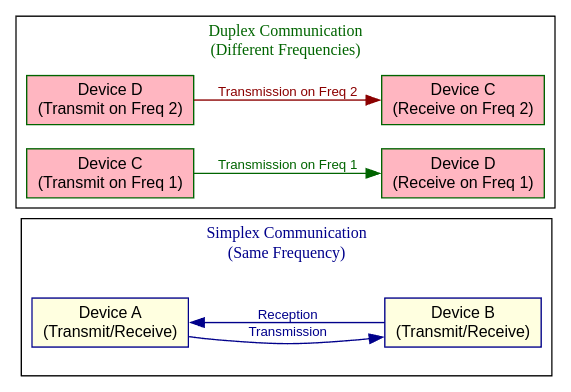
\includegraphics[width=0.8\textwidth]{simplex_duplex_diagram}
    \caption{Simplex vs. Duplex Communication}
    \label{fig:simplex_duplex}
    % Diagram illustrating the difference between simplex and duplex communication.
    % The diagram should show two scenarios: one where both transmission and reception occur on the same frequency (simplex), and another where transmission and reception occur on different frequencies (duplex).
\end{figure}

\begin{table}[h]
    \centering
    \caption{Simplex vs. Duplex Communication}
    \label{tab:simplex_duplex}
    \begin{tabular}{|l|l|}
        \hline
        \textbf{Communication Mode} & \textbf{Description} \\
        \hline
        Simplex & Transmission and reception occur on the same frequency. \\
        \hline
        Duplex & Transmission and reception occur on different frequencies. \\
        \hline
    \end{tabular}
\end{table}

\subsection*{CTCSS and DTMF Tones}
CTCSS (Continuous Tone-Coded Squelch System) and DTMF (Dual-Tone Multi-Frequency) tones are used in repeater operations to control access and improve communication quality. CTCSS tones are sub-audible tones transmitted along with normal voice audio to open the squelch of a receiver, ensuring that only signals with the correct tone are heard. DTMF tones, on the other hand, are used for remote control of repeaters and other equipment, allowing operators to perform functions like changing frequencies or activating features.

\subsection*{Linked Repeater Networks}
A linked repeater network is a system where multiple repeaters are interconnected, allowing signals received by one repeater to be transmitted by all the repeaters in the network. This extends the range of communication and enables operators to communicate over much larger areas than would be possible with a single repeater. Linked repeater networks are particularly useful in emergency situations where wide-area communication is essential.

\subsection*{Questions}
\begin{tcolorbox}[colback=gray!10!white,colframe=black!75!black,title={T2A09}]
    Which of the following indicates that a station is listening on a repeater and looking for a contact?
    \begin{enumerate}[label=\Alph*,noitemsep]
        \item “CQ CQ” followed by the repeater’s call sign
        \item \textbf{The station’s call sign followed by the word “monitoring”}
        \item The repeater call sign followed by the station’s call sign
        \item “QSY” followed by your call sign
    \end{enumerate}
\end{tcolorbox}
When a station is monitoring a repeater and looking for a contact, it typically identifies itself by its call sign followed by the word "monitoring." This indicates that the station is listening and available for communication.

%memory_trick T2A09

\begin{tcolorbox}[colback=gray!10!white,colframe=black!75!black,title={T2A10}]
    What is a band plan, beyond the privileges established by the FCC?
    \begin{enumerate}[label=\Alph*,noitemsep]
        \item \textbf{A voluntary guideline for using different modes or activities within an amateur band}
        \item A list of operating schedules
        \item A list of available net frequencies
        \item A plan devised by a club to indicate frequency band usage
    \end{enumerate}
\end{tcolorbox}
A band plan is a voluntary guideline that helps amateur radio operators organize their use of the frequency spectrum. It is not enforced by the FCC but is widely adopted to ensure efficient and harmonious use of the available frequencies.

%memory_trick T2A10

\begin{tcolorbox}[colback=gray!10!white,colframe=black!75!black,title={T2A11}]
    What term describes an amateur station that is transmitting and receiving on the same frequency?
    \begin{enumerate}[label=\Alph*,noitemsep]
        \item Full duplex
        \item Diplex
        \item \textbf{Simplex}
        \item Multiplex
    \end{enumerate}
\end{tcolorbox}
Simplex communication involves transmitting and receiving on the same frequency. This is commonly used for direct communication between two stations without the need for a repeater.

%memory_trick T2A11

\begin{tcolorbox}[colback=gray!10!white,colframe=black!75!black,title={T2A12}]
    What should you do before calling CQ?
    \begin{enumerate}[label=\Alph*,noitemsep]
        \item Listen first to be sure that no one else is using the frequency
        \item Ask if the frequency is in use
        \item Make sure you are authorized to use that frequency
        \item \textbf{All these choices are correct}
    \end{enumerate}
\end{tcolorbox}
Before calling CQ, it is important to listen to ensure the frequency is not in use, ask if the frequency is in use, and confirm that you are authorized to use that frequency. All these steps are essential to avoid interference and ensure proper operation.

%memory_trick T2A12

\begin{tcolorbox}[colback=gray!10!white,colframe=black!75!black,title={T2B01}]
    How is a VHF/UHF transceiver’s “reverse” function used?
    \begin{enumerate}[label=\Alph*,noitemsep]
        \item To reduce power output
        \item To increase power output
        \item \textbf{To listen on a repeater’s input frequency}
        \item To listen on a repeater’s output frequency
    \end{enumerate}
\end{tcolorbox}
The "reverse" function on a VHF/UHF transceiver is used to listen on a repeater's input frequency. This allows the operator to hear what is being transmitted directly to the repeater, which can be useful for troubleshooting or monitoring.

%memory_trick T2B01

\begin{tcolorbox}[colback=gray!10!white,colframe=black!75!black,title={T2B02}]
    What term describes the use of a sub-audible tone transmitted along with normal voice audio to open the squelch of a receiver?
    \begin{enumerate}[label=\Alph*,noitemsep]
        \item Carrier squelch
        \item Tone burst
        \item DTMF
        \item \textbf{CTCSS}
    \end{enumerate}
\end{tcolorbox}
CTCSS (Continuous Tone-Coded Squelch System) uses a sub-audible tone transmitted along with normal voice audio to open the squelch of a receiver. This ensures that only signals with the correct tone are heard, reducing interference from other transmissions.

%memory_trick T2B02

\begin{tcolorbox}[colback=gray!10!white,colframe=black!75!black,title={T2B03}]
    Which of the following describes a linked repeater network?
    \begin{enumerate}[label=\Alph*,noitemsep]
        \item \textbf{A network of repeaters in which signals received by one repeater are transmitted by all the repeaters in the network}
        \item A single repeater with more than one receiver
        \item Multiple repeaters with the same control operator
        \item A system of repeaters linked by APRS
    \end{enumerate}
\end{tcolorbox}
A linked repeater network is a system where multiple repeaters are interconnected, allowing signals received by one repeater to be transmitted by all the repeaters in the network. This extends the range of communication and is particularly useful in emergency situations.

%memory_trick T2B03

\begin{tcolorbox}[colback=gray!10!white,colframe=black!75!black,title={T2B04}]
    Which of the following could be the reason you are unable to access a repeater whose output you can hear?
    \begin{enumerate}[label=\Alph*,noitemsep]
        \item Improper transceiver offset
        \item You are using the wrong CTCSS tone
        \item You are using the wrong DCS code
        \item \textbf{All these choices are correct}
    \end{enumerate}
\end{tcolorbox}
If you can hear a repeater's output but cannot access it, the issue could be due to an improper transceiver offset, using the wrong CTCSS tone, or using the wrong DCS code. All these factors can prevent successful communication with the repeater.

%memory_trick T2B04

\subsection*{Summary}
\begin{itemize}
    \item \textbf{Band Plans}: Voluntary guidelines for organizing the use of different modes and activities within amateur radio bands.
    \item \textbf{Simplex vs. Duplex}: Simplex involves transmitting and receiving on the same frequency, while duplex uses separate frequencies for transmission and reception.
    \item \textbf{CTCSS and DTMF Tones}: Used in repeater operations to control access and improve communication quality.
    \item \textbf{Linked Repeater Networks}: Systems where multiple repeaters are interconnected to extend communication range and improve reliability.
\end{itemize}

\section{Advanced Operating Techniques}
\label{section:advanced_operating}

\subsection*{FM Transmission Distortion}
FM transmission distortion on voice peaks can occur when the input audio signal is too loud, causing over-modulation. This results in distorted audio at the receiving end. To avoid this, ensure that your microphone gain is properly adjusted and avoid speaking too loudly into the microphone. Over-modulation can also be caused by excessive transmit power, but this is less common in modern equipment.

\subsection*{DTMF Signaling}
Dual-Tone Multi-Frequency (DTMF) signaling uses pairs of audio tones to represent numbers, letters, or special characters. This signaling method is commonly used in amateur radio for remote control of repeaters, accessing voicemail systems, and other automated functions. Each DTMF tone is a combination of two frequencies, one from a low-frequency group and one from a high-frequency group.

\subsection*{Digital Repeater Talkgroups}
To join a digital repeater's talkgroup, you need to program your radio with the group's ID or code. Talkgroups allow multiple users to communicate on the same digital repeater without interfering with each other. Each talkgroup has a unique identifier, and your radio must be configured to use the correct ID to access the group. This system is commonly used in DMR (Digital Mobile Radio) networks.

\subsection*{Frequency Interference Management}
When two stations transmit on the same frequency and interfere with each other, they should negotiate continued use of the frequency. This is a common practice in amateur radio to ensure fair and efficient use of the spectrum. The Q signal \textbf{QRM} indicates that you are receiving interference from other stations, while \textbf{QSY} indicates that you are changing frequency to avoid interference.

\begin{figure}[h]
    \centering
    % 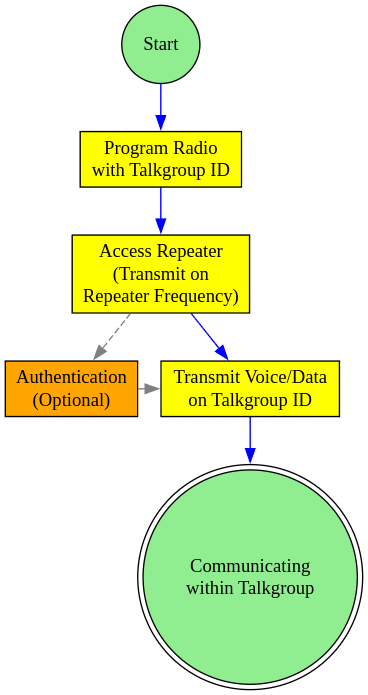
\includegraphics[width=0.8\textwidth]{figures/talkgroup.png}
    \caption{Joining a Digital Repeater Talkgroup}
    \label{fig:talkgroup}
    % Diagram showing the process of joining a digital repeater talkgroup. The diagram should include steps like programming the radio with the group ID, accessing the repeater, and communicating within the talkgroup.
\end{figure}

\begin{table}[h]
    \centering
    \begin{tabular}{|c|l|}
        \hline
        \textbf{Q Signal} & \textbf{Meaning} \\
        \hline
        QRM & Interference from other stations \\
        QSY & Changing frequency \\
        QTH & Location \\
        QSB & Fading signal \\
        \hline
    \end{tabular}
    \caption{Common Q Signals}
    \label{tab:q_signals}
\end{table}

\subsection*{Questions}
\begin{tcolorbox}[colback=gray!10!white,colframe=black!75!black,title={T2B05}]
    What would cause your FM transmission audio to be distorted on voice peaks?
    \begin{enumerate}[label=\Alph*,noitemsep]
        \item Your repeater offset is inverted
        \item You need to talk louder
        \item \textbf{You are talking too loudly}
        \item Your transmit power is too high
    \end{enumerate}
\end{tcolorbox}
Distortion on voice peaks in FM transmission is typically caused by over-modulation, which occurs when the input audio signal is too loud. This can be avoided by adjusting the microphone gain and speaking at a normal volume. Excessive transmit power is less likely to cause distortion in modern equipment.

%memory_trick T2B05

\begin{tcolorbox}[colback=gray!10!white,colframe=black!75!black,title={T2B06}]
    What type of signaling uses pairs of audio tones?
    \begin{enumerate}[label=\Alph*,noitemsep]
        \item \textbf{DTMF}
        \item CTCSS
        \item GPRS
        \item D-STAR
    \end{enumerate}
\end{tcolorbox}
DTMF (Dual-Tone Multi-Frequency) signaling uses pairs of audio tones to represent numbers, letters, or special characters. This method is widely used in amateur radio for remote control and automated systems.

%memory_trick T2B06

\begin{tcolorbox}[colback=gray!10!white,colframe=black!75!black,title={T2B07}]
    How can you join a digital repeater’s “talkgroup”?
    \begin{enumerate}[label=\Alph*,noitemsep]
        \item Register your radio with the local FCC office
        \item Join the repeater owner’s club
        \item \textbf{Program your radio with the group’s ID or code}
        \item Sign your call after the courtesy tone
    \end{enumerate}
\end{tcolorbox}
To join a digital repeater's talkgroup, you need to program your radio with the group's ID or code. This allows you to communicate within the designated group without interfering with other users on the same repeater.

%memory_trick T2B07

\begin{tcolorbox}[colback=gray!10!white,colframe=black!75!black,title={T2B08}]
    Which of the following applies when two stations transmitting on the same frequency interfere with each other?
    \begin{enumerate}[label=\Alph*,noitemsep]
        \item \textbf{The stations should negotiate continued use of the frequency}
        \item Both stations should choose another frequency to avoid conflict
        \item Interference is inevitable, so no action is required
        \item Use subaudible tones so both stations can share the frequency
    \end{enumerate}
\end{tcolorbox}
When two stations interfere on the same frequency, they should negotiate to determine who will continue using the frequency. This is a common practice in amateur radio to ensure fair use of the spectrum.

%memory_trick T2B08

\begin{tcolorbox}[colback=gray!10!white,colframe=black!75!black,title={T2B09}]
    Why are simplex channels designated in the VHF/UHF band plans?
    \begin{enumerate}[label=\Alph*,noitemsep]
        \item \textbf{So stations within range of each other can communicate without tying up a repeater}
        \item For contest operation
        \item For working DX only
        \item So stations with simple transmitters can access the repeater without automated offset
    \end{enumerate}
\end{tcolorbox}
Simplex channels are designated in the VHF/UHF band plans to allow stations within range of each other to communicate directly without using a repeater. This is useful for local communication and reduces the load on repeater systems.

%memory_trick T2B09

\begin{tcolorbox}[colback=gray!10!white,colframe=black!75!black,title={T2B10}]
    Which Q signal indicates that you are receiving interference from other stations?
    \begin{enumerate}[label=\Alph*,noitemsep]
        \item \textbf{QRM}
        \item QRN
        \item QTH
        \item QSB
    \end{enumerate}
\end{tcolorbox}
The Q signal \textbf{QRM} indicates that you are receiving interference from other stations. This is a common issue in crowded frequency bands, and operators may need to change frequencies to avoid the interference.

%memory_trick T2B10

\begin{tcolorbox}[colback=gray!10!white,colframe=black!75!black,title={T2B11}]
    Which Q signal indicates that you are changing frequency?
    \begin{enumerate}[label=\Alph*,noitemsep]
        \item QRU
        \item \textbf{QSY}
        \item QSL
        \item QRZ
    \end{enumerate}
\end{tcolorbox}
The Q signal \textbf{QSY} indicates that you are changing frequency. This is often used to avoid interference or to move to a clearer frequency for communication.

%memory_trick T2B11

\begin{tcolorbox}[colback=gray!10!white,colframe=black!75!black,title={T2B12}]
    What is the purpose of the color code used on DMR repeater systems?
    \begin{enumerate}[label=\Alph*,noitemsep]
        \item \textbf{Must match the repeater color code for access}
        \item Defines the frequency pair to use
        \item Identifies the codec used
        \item Defines the minimum signal level required for access
    \end{enumerate}
\end{tcolorbox}
The color code in DMR repeater systems is used to ensure that your radio matches the repeater's color code for access. This helps prevent unauthorized access and ensures compatibility between radios and repeaters.

%memory_trick T2B12

\subsection*{Summary}
This section covered advanced operating techniques in amateur radio, including:
\begin{itemize}
    \item \textbf{FM Transmission Distortion}: Caused by over-modulation due to excessive audio input. Adjust microphone gain to avoid distortion.
    \item \textbf{DTMF Signaling}: Uses pairs of audio tones for remote control and automated functions in amateur radio.
    \item \textbf{Digital Repeater Talkgroups}: Join by programming your radio with the group's ID or code to communicate within a specific group.
    \item \textbf{Frequency Interference Management}: Use Q signals like QRM and QSY to manage and avoid interference on shared frequencies.
\end{itemize}

\section{Emergency Operations and Traffic Handling}
\label{section:emergency_operations}

\subsection*{Introduction}
In emergency situations, amateur radio operators play a critical role in maintaining communication when traditional systems fail. This section discusses the application of FCC rules during emergencies, the duties of a Net Control Station, the importance of using a phonetic alphabet, and best practices for traffic handling.

\subsection*{FCC Rules in Emergencies}
The FCC rules are designed to ensure orderly and efficient communication, especially during emergencies. These rules apply to all amateur radio operations, including those conducted under the Radio Amateur Civil Emergency Service (RACES) and the Amateur Radio Emergency Service (ARES). The FCC rules provide a framework for emergency communications, ensuring that all operators adhere to standardized procedures.

\subsection*{Duties of a Net Control Station}
A Net Control Station (NCS) is responsible for managing communications during an emergency net. The primary duties of an NCS include:
\begin{itemize}
    \item Calling the net to order and directing communications between stations.
    \item Ensuring that all stations checking into the net are properly licensed.
    \item Coordinating the exchange of messages and ensuring that traffic is handled efficiently.
\end{itemize}

\subsection*{Importance of Phonetic Alphabet}
Clear communication is essential in emergency situations. The use of a standard phonetic alphabet ensures that voice messages containing unusual or technical words are received correctly. For example, the word "Bravo" is used to represent the letter "B," reducing the likelihood of miscommunication.

\begin{table}[h]
    \centering
    \caption{Phonetic Alphabet}
    \label{tab:phonetic_alphabet}
    \begin{tabular}{|c|c|}
        \hline
        \textbf{Letter} & \textbf{Phonetic Representation} \\
        \hline
        A & Alpha \\
        B & Bravo \\
        C & Charlie \\
        D & Delta \\
        \hline
    \end{tabular}
\end{table}

\subsection*{Traffic Handling Best Practices}
Effective traffic handling is crucial for the smooth operation of an emergency net. Key characteristics of good traffic handling include:
\begin{itemize}
    \item Passing messages exactly as received.
    \item Avoiding unnecessary modifications or interpretations of messages.
    \item Ensuring that messages are relayed promptly and accurately.
\end{itemize}

\begin{figure}[h]
    \centering
    % \includegraphics[width=0.8\textwidth]{traffic_handling_flowchart}
    \caption{Traffic Handling Process}
    \label{fig:traffic_handling}
    % Prompt: Flowchart showing the process of handling traffic in an emergency net.
    % The figure should include steps such as message reception, verification, and relay.
\end{figure}

\subsection*{Questions}
\begin{tcolorbox}[colback=gray!10!white,colframe=black!75!black,title={T2C01}]
    When do FCC rules NOT apply to the operation of an amateur station?
    \begin{enumerate}[label=\Alph*,noitemsep]
        \item When operating a RACES station
        \item When operating under special FEMA rules
        \item When operating under special ARES rules
        \item \textbf{FCC rules always apply}
    \end{enumerate}
\end{tcolorbox}
FCC rules are always applicable to amateur radio operations, regardless of the situation. This ensures consistency and reliability in communications, especially during emergencies.

%memory_trick T2C01

\begin{tcolorbox}[colback=gray!10!white,colframe=black!75!black,title={T2C02}]
    Which of the following are typical duties of a Net Control Station?
    \begin{enumerate}[label=\Alph*,noitemsep]
        \item Choose the regular net meeting time and frequency
        \item Ensure that all stations checking into the net are properly licensed for operation on the net frequency
        \item \textbf{Call the net to order and direct communications between stations checking in}
        \item All these choices are correct
    \end{enumerate}
\end{tcolorbox}
The primary duty of a Net Control Station is to manage communications during a net, including calling the net to order and directing communications. Licensing verification is typically handled by the FCC, not the NCS.

%memory_trick T2C02

\begin{tcolorbox}[colback=gray!10!white,colframe=black!75!black,title={T2C03}]
    What technique is used to ensure that voice messages containing unusual words are received correctly?
    \begin{enumerate}[label=\Alph*,noitemsep]
        \item Send the words by voice and Morse code
        \item Speak very loudly into the microphone
        \item \textbf{Spell the words using a standard phonetic alphabet}
        \item All these choices are correct
    \end{enumerate}
\end{tcolorbox}
Using a phonetic alphabet ensures clarity in communication, especially for unusual or technical terms. This reduces the likelihood of misunderstandings.

%memory_trick T2C03

\subsection*{Summary}
This section covered the following key concepts:
\begin{itemize}
    \item \textbf{FCC rules in emergencies}: FCC rules always apply to amateur radio operations, ensuring consistency and reliability.
    \item \textbf{Net control station duties}: The NCS manages communications, directs traffic, and ensures orderly operations.
    \item \textbf{Phonetic alphabet usage}: A standard phonetic alphabet is essential for clear communication.
    \item \textbf{Traffic handling best practices}: Messages should be passed exactly as received, without unnecessary modifications.
\end{itemize}

\section{Message Handling and Radiograms}
\label{section:message_handling}

\subsection*{Message Handling and Radiograms}

Amateur radio operators play a crucial role in emergency communication, and understanding the rules and procedures for message handling is essential. This section covers the circumstances under which operators can operate outside their licensed frequency privileges, the structure of radiograms, and the purpose of the squelch function in receivers.

\subsection*{Frequency Privileges in Emergencies}

Amateur station control operators are generally required to operate within the frequency privileges of their license class. However, there are exceptions in situations involving the immediate safety of human life or protection of property. According to FCC regulations, operators may operate outside their licensed privileges in such emergencies. This flexibility ensures that amateur radio can be effectively used in critical situations where communication is vital.

\subsection*{Radiogram Preamble}

The preamble of a formal traffic message contains essential information needed to track and manage the message. This includes details such as the message number, precedence, handling instructions, and the station of origin. The preamble ensures that the message can be properly routed and delivered, even in complex networks.

\begin{table}[h]
    \centering
    \caption{Radiogram Preamble Components}
    \label{tab:radiogram_preamble}
    \begin{tabular}{|l|l|}
        \hline
        \textbf{Component} & \textbf{Description} \\
        \hline
        Message Number & Unique identifier for the message \\
        Precedence & Indicates the urgency of the message \\
        Handling Instructions & Special instructions for handling the message \\
        Station of Origin & Call sign of the originating station \\
        \hline
    \end{tabular}
\end{table}

\subsection*{Meaning of 'Check' in a Radiogram Header}

The term "check" in a radiogram header refers to the number of words or word equivalents in the text portion of the message. This information is crucial for ensuring that the message is transmitted and received accurately. The check value helps operators verify that the entire message has been correctly relayed without omissions or errors.

\subsection*{Squelch Function}

The squelch function in a receiver is designed to mute the audio when no signal is present. This prevents the annoyance of hearing background noise when the receiver is not actively receiving a signal. By muting the audio in the absence of a signal, the squelch function improves the listening experience and reduces fatigue.

\begin{figure}[h]
    \centering
    % \includegraphics{radiogram_preamble_structure.png}
    \caption{Radiogram Preamble Structure}
    \label{fig:radiogram_preamble}
    % Diagram illustrating the structure of a radiogram preamble.
    % The diagram should show the components of the preamble, such as the message number, precedence, handling instructions, and station of origin.
\end{figure}

\subsection*{Questions}

\begin{tcolorbox}[colback=gray!10!white,colframe=black!75!black,title={T2C09}]
    Are amateur station control operators ever permitted to operate outside the frequency privileges of their license class?
    \begin{enumerate}[label=\Alph*,noitemsep]
        \item No
        \item Yes, but only when part of a FEMA emergency plan
        \item Yes, but only when part of a RACES emergency plan
        \item \textbf{Yes, but only in situations involving the immediate safety of human life or protection of property}
    \end{enumerate}
\end{tcolorbox}

Amateur operators are permitted to operate outside their licensed frequency privileges only in situations involving the immediate safety of human life or protection of property. This exception is crucial for emergency communications, where flexibility can save lives and protect property.

%memory_trick T2C09

\begin{tcolorbox}[colback=gray!10!white,colframe=black!75!black,title={T2C10}]
    What information is contained in the preamble of a formal traffic message?
    \begin{enumerate}[label=\Alph*,noitemsep]
        \item The email address of the originating station
        \item The address of the intended recipient
        \item The telephone number of the addressee
        \item \textbf{Information needed to track the message}
    \end{enumerate}
\end{tcolorbox}

The preamble of a formal traffic message contains information needed to track the message, such as the message number, precedence, handling instructions, and the station of origin. This ensures that the message can be properly routed and delivered.

%memory_trick T2C10

\begin{tcolorbox}[colback=gray!10!white,colframe=black!75!black,title={T2C11}]
    What is meant by "check" in a radiogram header?
    \begin{enumerate}[label=\Alph*,noitemsep]
        \item \textbf{The number of words or word equivalents in the text portion of the message}
        \item The call sign of the originating station
        \item A list of stations that have relayed the message
        \item A box on the message form that indicates that the message was received and/or relayed
    \end{enumerate}
\end{tcolorbox}

The "check" in a radiogram header refers to the number of words or word equivalents in the text portion of the message. This helps ensure that the message is transmitted and received accurately.

%memory_trick T2C11

\begin{tcolorbox}[colback=gray!10!white,colframe=black!75!black,title={T2B13}]
    What is the purpose of a squelch function?
    \begin{enumerate}[label=\Alph*,noitemsep]
        \item Reduce a CW transmitter's key clicks
        \item \textbf{Mute the receiver audio when a signal is not present}
        \item Eliminate parasitic oscillations in an RF amplifier
        \item Reduce interference from impulse noise
    \end{enumerate}
\end{tcolorbox}

The squelch function mutes the receiver audio when no signal is present, preventing the annoyance of background noise. This improves the listening experience and reduces fatigue.

%memory_trick T2B13

\subsection*{Summary}

This section covered key concepts related to message handling and radiograms in amateur radio:

\begin{itemize}
    \item \textbf{Frequency privileges in emergencies}: Operators may operate outside their licensed privileges in situations involving the immediate safety of human life or protection of property.
    \item \textbf{Radiogram preambles}: The preamble contains essential information needed to track and manage the message, such as the message number, precedence, handling instructions, and station of origin.
    \item \textbf{Message tracking}: The "check" in a radiogram header refers to the number of words or word equivalents in the text portion of the message, ensuring accurate transmission and reception.
    \item \textbf{Squelch function}: This function mutes the receiver audio when no signal is present, improving the listening experience by eliminating background noise.
\end{itemize}

\chapter{RADIO WAVE PROPAGATION}
\label{chapter:radio_wave_propagation}
\section{Signal Variability and Challenges}
\label{section:signal_variability}

\subsection*{Multipath Propagation}
Multipath propagation occurs when radio signals take multiple paths to reach the receiver due to reflections, refractions, and diffractions caused by obstacles such as buildings, hills, or other structures. This phenomenon can lead to signal cancellation or reinforcement, depending on the phase relationship between the arriving signals. For example, if two signals arrive at the receiver with a phase difference of 180 degrees, they will cancel each other out, resulting in a significant drop in signal strength. Conversely, if the signals arrive in phase, they will reinforce each other, increasing the signal strength. This is why VHF signal strengths can vary greatly when the antenna is moved only a few feet, as the relative phase of the multipath signals changes with the antenna's position.

\begin{figure}[h!]
    \centering
    % \includegraphics[width=0.8\textwidth]{multipath_propagation}
    \caption{Multipath propagation causing signal cancellation and reinforcement.}
    \label{fig:multipath_propagation}
    % Diagram showing multipath propagation effects on VHF signals. The figure should include a transmitter, receiver, and multiple signal paths reflecting off buildings and terrain, with annotations showing constructive and destructive interference.
\end{figure}

\subsection*{Signal Absorption by Vegetation}
Vegetation can significantly affect UHF and microwave signals by absorbing the radio waves. The water content in leaves and branches acts as a dielectric, absorbing the energy of the signal and reducing its strength. This effect is more pronounced at higher frequencies, such as UHF and microwave bands, where the wavelength is shorter and more easily absorbed by the vegetation. As a result, the range of communication can be reduced when the signal path passes through dense foliage.

\begin{figure}[h!]
    \centering
    % \includegraphics[width=0.8\textwidth]{vegetation_absorption}
    \caption{Effect of vegetation on UHF and microwave signals.}
    \label{fig:vegetation_absorption}
    % Illustration of signal absorption by vegetation. The figure should show a transmitter, receiver, and a forested area with signal strength decreasing as it passes through the trees.
\end{figure}

\subsection*{Antenna Polarization}
Antenna polarization is crucial for long-distance VHF and UHF communications. Horizontal polarization is typically used for long-distance CW (Continuous Wave) and SSB (Single Sideband) contacts because it is less susceptible to ground reflections and provides better performance over long distances. Vertical polarization, on the other hand, is often used for local communications, especially in mobile and portable setups, as it is more effective in urban environments where signals may reflect off buildings and other structures.

\subsection*{Mismatched Antenna Polarization}
When antennas at opposite ends of a VHF or UHF line-of-sight radio link are not using the same polarization, the received signal strength is significantly reduced. This is because the receiving antenna is not aligned with the polarization of the incoming signal, leading to a loss of signal energy. For optimal communication, both antennas should have the same polarization.

\subsection*{Overcoming Obstructions with Directional Antennas}
Directional antennas can be used to overcome obstructions in line-of-sight communication by reflecting signals off nearby structures or terrain. By adjusting the antenna's orientation, it is possible to find a path that reflects the signal toward the repeater, bypassing the obstruction. This technique is particularly useful in urban environments where buildings may block the direct line of sight.

\subsection*{Picket Fencing}
Picket fencing refers to the rapid flutter or variation in signal strength experienced by mobile stations due to multipath propagation. As the mobile station moves, the relative phase of the multipath signals changes, causing the signal to fluctuate rapidly. This effect is similar to the appearance of a picket fence when viewed from a moving vehicle, hence the name.

\subsection*{Weather Effects on Microwave Signals}
Precipitation, such as rain or snow, can significantly reduce the range of microwave signals. Water droplets in the atmosphere absorb and scatter the microwave energy, leading to signal attenuation. This effect is more pronounced at higher frequencies, where the wavelength is shorter and more easily absorbed by the water droplets.

\begin{table}[h!]
    \centering
    \begin{tabular}{|l|l|}
        \hline
        \textbf{Weather Condition} & \textbf{Effect on Signal Propagation} \\
        \hline
        High winds & Minimal effect on signal strength \\
        Low barometric pressure & Minimal effect on signal strength \\
        Precipitation & Significant signal attenuation \\
        Colder temperatures & Minimal effect on signal strength \\
        \hline
    \end{tabular}
    \caption{Weather effects on signal propagation.}
    \label{tab:weather_effects}
\end{table}

\subsection*{Irregular Fading in Ionospheric Signals}
Irregular fading of signals propagated by the ionosphere is often caused by the random combining of signals arriving via different paths. As the ionosphere is a dynamic and irregular medium, signals can take multiple paths with varying delays and phase shifts. When these signals combine at the receiver, they can interfere constructively or destructively, leading to rapid and irregular variations in signal strength.

\subsection*{Questions}

\begin{tcolorbox}[colback=gray!10!white,colframe=black!75!black,title={T3A01}]
    Why do VHF signal strengths sometimes vary greatly when the antenna is moved only a few feet?
    \begin{enumerate}[label=\Alph*,noitemsep]
        \item The signal path encounters different concentrations of water vapor
        \item VHF ionospheric propagation is very sensitive to path length
        \item \textbf{Multipath propagation cancels or reinforces signals}
        \item All these choices are correct
    \end{enumerate}
\end{tcolorbox}
Multipath propagation causes signals to arrive at the receiver via multiple paths, leading to constructive or destructive interference. Moving the antenna changes the relative phase of these signals, resulting in significant variations in signal strength.

%memory_trick T3A01

\begin{tcolorbox}[colback=gray!10!white,colframe=black!75!black,title={T3A02}]
    What is the effect of vegetation on UHF and microwave signals?
    \begin{enumerate}[label=\Alph*,noitemsep]
        \item Knife-edge diffraction
        \item \textbf{Absorption}
        \item Amplification
        \item Polarization rotation
    \end{enumerate}
\end{tcolorbox}
Vegetation absorbs UHF and microwave signals due to the water content in leaves and branches, reducing signal strength.

%memory_trick T3A02

\begin{tcolorbox}[colback=gray!10!white,colframe=black!75!black,title={T3A03}]
    What antenna polarization is normally used for long-distance CW and SSB contacts on the VHF and UHF bands?
    \begin{enumerate}[label=\Alph*,noitemsep]
        \item Right-hand circular
        \item Left-hand circular
        \item \textbf{Horizontal}
        \item Vertical
    \end{enumerate}
\end{tcolorbox}
Horizontal polarization is preferred for long-distance VHF and UHF communications because it is less affected by ground reflections and provides better performance over long distances.

%memory_trick T3A03

\begin{tcolorbox}[colback=gray!10!white,colframe=black!75!black,title={T3A04}]
    What happens when antennas at opposite ends of a VHF or UHF line of sight radio link are not using the same polarization?
    \begin{enumerate}[label=\Alph*,noitemsep]
        \item The modulation sidebands might become inverted
        \item \textbf{Received signal strength is reduced}
        \item Signals have an echo effect
        \item Nothing significant will happen
    \end{enumerate}
\end{tcolorbox}
Mismatched polarization leads to a reduction in received signal strength because the receiving antenna is not aligned with the polarization of the incoming signal.

%memory_trick T3A04

\begin{tcolorbox}[colback=gray!10!white,colframe=black!75!black,title={T3A05}]
    When using a directional antenna, how might your station be able to communicate with a distant repeater if buildings or obstructions are blocking the direct line of sight path?
    \begin{enumerate}[label=\Alph*,noitemsep]
        \item Change from vertical to horizontal polarization
        \item \textbf{Try to find a path that reflects signals to the repeater}
        \item Try the long path
        \item Increase the antenna SWR
    \end{enumerate}
\end{tcolorbox}
Directional antennas can reflect signals off nearby structures or terrain to bypass obstructions, allowing communication with the repeater.

%memory_trick T3A05

\begin{tcolorbox}[colback=gray!10!white,colframe=black!75!black,title={T3A06}]
    What is the meaning of the term “picket fencing”?
    \begin{enumerate}[label=\Alph*,noitemsep]
        \item Alternating transmissions during a net operation
        \item \textbf{Rapid flutter on mobile signals due to multipath propagation}
        \item A type of ground system used with vertical antennas
        \item Local vs long-distance communications
    \end{enumerate}
\end{tcolorbox}
Picket fencing refers to the rapid flutter in signal strength experienced by mobile stations due to multipath propagation.

%memory_trick T3A06

\begin{tcolorbox}[colback=gray!10!white,colframe=black!75!black,title={T3A07}]
    What weather condition might decrease range at microwave frequencies?
    \begin{enumerate}[label=\Alph*,noitemsep]
        \item High winds
        \item Low barometric pressure
        \item \textbf{Precipitation}
        \item Colder temperatures
    \end{enumerate}
\end{tcolorbox}
Precipitation, such as rain or snow, absorbs and scatters microwave signals, leading to signal attenuation and reduced range.

%memory_trick T3A07

\begin{tcolorbox}[colback=gray!10!white,colframe=black!75!black,title={T3A08}]
    What is a likely cause of irregular fading of signals propagated by the ionosphere?
    \begin{enumerate}[label=\Alph*,noitemsep]
        \item Frequency shift due to Faraday rotation
        \item Interference from thunderstorms
        \item Intermodulation distortion
        \item \textbf{Random combining of signals arriving via different paths}
    \end{enumerate}
\end{tcolorbox}
Irregular fading is caused by the random combination of signals arriving via different paths through the ionosphere, leading to constructive or destructive interference.

%memory_trick T3A08

\subsection*{Summary}
This section discussed several key concepts related to signal variability and challenges in radio communication:
\begin{itemize}
    \item \textbf{Multipath propagation}: Causes signal cancellation or reinforcement due to multiple signal paths.
    \item \textbf{Signal absorption}: Vegetation absorbs UHF and microwave signals, reducing their strength.
    \item \textbf{Antenna polarization}: Horizontal polarization is preferred for long-distance VHF and UHF communications.
    \item \textbf{Signal reflection}: Directional antennas can reflect signals to overcome obstructions.
    \item \textbf{Picket fencing}: Rapid signal flutter due to multipath propagation in mobile communications.
    \item \textbf{Weather effects}: Precipitation can significantly reduce microwave signal range.
    \item \textbf{Irregular fading}: Caused by random combining of signals arriving via different ionospheric paths.
\end{itemize}

\section{Electromagnetic Essentials}
\label{section:electromagnetic_essentials}

\subsection*{Introduction}
This section covers the fundamental concepts of electromagnetic waves, including the relationship between electric and magnetic fields, wave polarization, the velocity of radio waves, and the relationship between wavelength and frequency. These concepts are essential for understanding how radio waves propagate and how they are used in amateur radio.

\subsection*{Electric and Magnetic Fields}
An electromagnetic wave consists of two perpendicular components: an electric field and a magnetic field. These fields oscillate at right angles to each other and to the direction of wave propagation. The relationship between the electric and magnetic fields is such that they are always perpendicular to each other, as shown in Figure~\ref{fig:em_fields}.

\begin{figure}[h!]
    \centering
    % \includegraphics[width=0.8\textwidth]{em_fields.svg}
    \caption{Electric and magnetic fields in an electromagnetic wave.}
    \label{fig:em_fields}
    % Diagram showing the relationship between electric and magnetic fields in an electromagnetic wave.
    % The electric field (E) is vertical, and the magnetic field (B) is horizontal, both perpendicular to the direction of propagation (k).
\end{figure}

\subsection*{Wave Polarization}
The polarization of a radio wave is defined by the orientation of its electric field. For example, if the electric field oscillates vertically, the wave is said to be vertically polarized. Conversely, if the electric field oscillates horizontally, the wave is horizontally polarized. The magnetic field is always perpendicular to the electric field and does not determine polarization.

\subsection*{Components of a Radio Wave}
A radio wave consists of two primary components: the electric field and the magnetic field. These fields are interdependent and propagate together through space. The electric field is responsible for the wave's interaction with matter, while the magnetic field plays a role in the wave's energy transfer.

\subsection*{Velocity of Radio Waves}
In free space, radio waves travel at the speed of light, which is approximately $3 \times 10^8$ meters per second. This velocity is constant and does not depend on the frequency or wavelength of the wave.

\subsection*{Wavelength and Frequency Relationship}
The wavelength ($\lambda$) and frequency ($f$) of a radio wave are inversely related. This relationship is expressed by the formula:
\begin{equation}
    \lambda = \frac{c}{f}
    \label{eq:wavelength_frequency}
\end{equation}
where $c$ is the speed of light. As frequency increases, wavelength decreases, and vice versa. This relationship is illustrated in Figure~\ref{fig:wavelength_frequency}.

\begin{figure}[h!]
    \centering
    % \includegraphics[width=0.8\textwidth]{wavelength_frequency.png}
    \caption{Wavelength vs. frequency relationship.}
    \label{fig:wavelength_frequency}
    % Graph showing the inverse relationship between wavelength and frequency.
    % The x-axis represents frequency (Hz), and the y-axis represents wavelength (m).
\end{figure}

\subsection*{Frequency to Wavelength Conversion}
To convert frequency to wavelength in meters, the following formula is used:
\begin{equation}
    \lambda = \frac{300}{f_{\text{MHz}}}
    \label{eq:frequency_wavelength}
\end{equation}
where $f_{\text{MHz}}$ is the frequency in megahertz. For example, a frequency of 150 MHz corresponds to a wavelength of 2 meters.

\subsection*{Amateur Radio Band Identification}
Amateur radio bands are often identified by their approximate wavelength in meters. For example, the 2-meter band corresponds to frequencies around 144 MHz. Table~\ref{tab:frequency_ranges} summarizes the frequency ranges for VHF, UHF, and HF bands.

\begin{table}[h!]
    \centering
    \begin{tabular}{|c|c|}
        \hline
        \textbf{Band} & \textbf{Frequency Range} \\
        \hline
        VHF & 30 MHz to 300 MHz \\
        UHF & 300 MHz to 3000 MHz \\
        HF & 3 MHz to 30 MHz \\
        \hline
    \end{tabular}
    \caption{Frequency ranges for amateur radio bands.}
    \label{tab:frequency_ranges}
\end{table}

\subsection*{Questions}
\begin{tcolorbox}[colback=gray!10!white,colframe=black!75!black,title={T3B01}]
    What is the relationship between the electric and magnetic fields of an electromagnetic wave?
    \begin{enumerate}[label=\Alph*),noitemsep]
        \item They travel at different speeds
        \item They are in parallel
        \item They revolve in opposite directions
        \item \textbf{They are at right angles}
    \end{enumerate}
\end{tcolorbox}
The electric and magnetic fields of an electromagnetic wave are always perpendicular to each other and to the direction of propagation. This is a fundamental property of electromagnetic waves.

%memory_trick T3B01

\begin{tcolorbox}[colback=gray!10!white,colframe=black!75!black,title={T3B02}]
    What property of a radio wave defines its polarization?
    \begin{enumerate}[label=\Alph*),noitemsep]
        \item \textbf{The orientation of the electric field}
        \item The orientation of the magnetic field
        \item The ratio of the energy in the magnetic field to the energy in the electric field
        \item The ratio of the velocity to the wavelength
    \end{enumerate}
\end{tcolorbox}
Polarization is determined by the orientation of the electric field. The magnetic field is always perpendicular to the electric field and does not influence polarization.

%memory_trick T3B02

\begin{tcolorbox}[colback=gray!10!white,colframe=black!75!black,title={T3B03}]
    What are the two components of a radio wave?
    \begin{enumerate}[label=\Alph*),noitemsep]
        \item Impedance and reactance
        \item Voltage and current
        \item \textbf{Electric and magnetic fields}
        \item Ionizing and non-ionizing radiation
    \end{enumerate}
\end{tcolorbox}
A radio wave consists of electric and magnetic fields that propagate together through space. These fields are interdependent and oscillate perpendicular to each other.

%memory_trick T3B03

\begin{tcolorbox}[colback=gray!10!white,colframe=black!75!black,title={T3B04}]
    What is the velocity of a radio wave traveling through free space?
    \begin{enumerate}[label=\Alph*),noitemsep]
        \item \textbf{Speed of light}
        \item Speed of sound
        \item Speed inversely proportional to its wavelength
        \item Speed that increases as the frequency increases
    \end{enumerate}
\end{tcolorbox}
Radio waves travel at the speed of light in free space, which is approximately $3 \times 10^8$ meters per second. This speed is constant and does not depend on the wave's frequency or wavelength.

%memory_trick T3B04

\begin{tcolorbox}[colback=gray!10!white,colframe=black!75!black,title={T3B05}]
    What is the relationship between wavelength and frequency?
    \begin{enumerate}[label=\Alph*),noitemsep]
        \item Wavelength gets longer as frequency increases
        \item \textbf{Wavelength gets shorter as frequency increases}
        \item Wavelength and frequency are unrelated
        \item Wavelength and frequency increase as path length increases
    \end{enumerate}
\end{tcolorbox}
Wavelength and frequency are inversely related. As frequency increases, wavelength decreases, and vice versa. This relationship is described by the formula $\lambda = \frac{c}{f}$.

%memory_trick T3B05

\begin{tcolorbox}[colback=gray!10!white,colframe=black!75!black,title={T3B06}]
    What is the formula for converting frequency to approximate wavelength in meters?
    \begin{enumerate}[label=\Alph*),noitemsep]
        \item Wavelength in meters equals frequency in hertz multiplied by 300
        \item Wavelength in meters equals frequency in hertz divided by 300
        \item Wavelength in meters equals frequency in megahertz divided by 300
        \item \textbf{Wavelength in meters equals 300 divided by frequency in megahertz}
    \end{enumerate}
\end{tcolorbox}
The correct formula for converting frequency to wavelength in meters is $\lambda = \frac{300}{f_{\text{MHz}}}$. This formula is derived from the relationship $\lambda = \frac{c}{f}$, where $c$ is the speed of light.

%memory_trick T3B06

\begin{tcolorbox}[colback=gray!10!white,colframe=black!75!black,title={T3B07}]
    In addition to frequency, which of the following is used to identify amateur radio bands?
    \begin{enumerate}[label=\Alph*),noitemsep]
        \item \textbf{The approximate wavelength in meters}
        \item Traditional letter/number designators
        \item Channel numbers
        \item All these choices are correct
    \end{enumerate}
\end{tcolorbox}
Amateur radio bands are often identified by their approximate wavelength in meters. For example, the 2-meter band corresponds to frequencies around 144 MHz.

%memory_trick T3B07

\begin{tcolorbox}[colback=gray!10!white,colframe=black!75!black,title={T3B08}]
    What frequency range is referred to as VHF?
    \begin{enumerate}[label=\Alph*),noitemsep]
        \item 30 kHz to 300 kHz
        \item \textbf{30 MHz to 300 MHz}
        \item 300 kHz to 3000 kHz
        \item 300 MHz to 3000 MHz
    \end{enumerate}
\end{tcolorbox}
The VHF (Very High Frequency) range spans from 30 MHz to 300 MHz. This range is commonly used for FM radio, television broadcasting, and amateur radio.

%memory_trick T3B08

\subsection*{Summary}
This section introduced the essential concepts of electromagnetic waves, including:
\begin{itemize}
    \item \textbf{Electric and magnetic fields}: These fields are perpendicular to each other and to the direction of wave propagation.
    \item \textbf{Wave polarization}: Determined by the orientation of the electric field.
    \item \textbf{Velocity of radio waves}: Radio waves travel at the speed of light in free space.
    \item \textbf{Wavelength and frequency relationship}: Wavelength and frequency are inversely related.
    \item \textbf{Frequency to wavelength conversion}: The formula $\lambda = \frac{300}{f_{\text{MHz}}}$ is used to convert frequency to wavelength in meters.
    \item \textbf{Amateur radio band identification}: Bands are often identified by their approximate wavelength in meters.
\end{itemize}

\section{Propagation Basics}
\label{section:propagation_basics}

\subsection*{UHF Signal Propagation}
UHF signals are rarely heard beyond the radio horizon due to their limited propagation characteristics. Unlike lower frequency signals, UHF signals are not typically reflected or refracted by the ionosphere. Instead, they propagate primarily via line-of-sight, which restricts their range to the visual horizon. This is illustrated in Figure~\ref{fig:uhf_propagation}, which shows how UHF signals are absorbed or scattered by the Earth's atmosphere and terrain.

% Insert figure for UHF propagation
\begin{figure}[h!]
    \centering
    % \includegraphics[width=0.8\textwidth]{figures/uhf_propagation.svg}
    \caption{UHF signal propagation and horizon limitations.}
    \label{fig:uhf_propagation}
    % Prompt: Diagram illustrating UHF signal propagation limitations, showing how signals are absorbed or scattered by the atmosphere and terrain.
\end{figure}

\subsection*{HF vs. VHF Communication}
High-frequency (HF) communication differs significantly from very high-frequency (VHF) and ultra high-frequency (UHF) communication. HF signals (3–30 MHz) are capable of long-distance ionospheric propagation, allowing them to travel thousands of kilometers by reflecting off the ionosphere. In contrast, VHF and UHF signals (30 MHz and above) are primarily limited to line-of-sight propagation, making them less suitable for long-distance communication.

\subsection*{Auroral Backscatter}
VHF signals received via auroral backscatter exhibit unique characteristics. These signals are often distorted, and their strength varies considerably due to the irregular nature of the auroral ionization. This phenomenon occurs when VHF signals are scattered by the ionized regions of the aurora, resulting in fluctuating signal quality.

\subsection*{Sporadic E Propagation}
Sporadic E propagation is a key mechanism for occasional strong signals on the 10, 6, and 2-meter bands from beyond the radio horizon. This phenomenon occurs when dense patches of ionization form in the E layer of the ionosphere, reflecting VHF signals over long distances. Sporadic E is particularly common during summer months and can enable communication over hundreds or even thousands of kilometers.

\subsection*{Knife-Edge Diffraction}
Knife-edge diffraction allows radio signals to travel beyond obstructions such as mountains or buildings. When a signal encounters a sharp edge, it bends around the obstacle, enabling communication even when there is no direct line of sight. This effect is particularly useful in mountainous or urban environments where obstacles would otherwise block the signal.

\subsection*{Tropospheric Ducting}
Tropospheric ducting is a propagation mechanism that enables over-the-horizon VHF and UHF communication, often extending ranges up to 300 miles. This phenomenon occurs when temperature inversions in the troposphere create a duct-like layer that traps and guides radio waves. Figure~\ref{fig:tropospheric_ducting} illustrates the mechanism of tropospheric ducting.

% Insert figure for tropospheric ducting
\begin{figure}[h!]
    \centering
    % \includegraphics[width=0.8\textwidth]{figures/tropospheric_ducting.svg}
    \caption{Tropospheric ducting mechanism.}
    \label{fig:tropospheric_ducting}
    % Prompt: Illustration of tropospheric ducting, showing how temperature inversions create a duct-like layer that traps and guides radio waves.
\end{figure}

\subsection*{Meteor Scatter}
The 6-meter band is particularly well-suited for meteor scatter communication. When meteors enter the Earth's atmosphere, they create ionized trails that can reflect VHF signals. These trails are short-lived but can enable communication over distances of up to 1,500 kilometers.

\subsection*{Temperature Inversions}
Temperature inversions in the atmosphere are the primary cause of tropospheric ducting. These inversions occur when a layer of warm air lies above a layer of cooler air, creating a boundary that reflects radio waves back toward the Earth's surface.

\subsection*{Propagation Mechanisms Summary}
Table~\ref{tab:propagation_mechanisms} summarizes the different propagation mechanisms and their characteristics.

% Insert table for propagation mechanisms
\begin{table}[h!]
    \centering
    \begin{tabular}{|l|l|}
        \hline
        \textbf{Mechanism} & \textbf{Characteristics} \\
        \hline
        UHF Propagation & Limited to line-of-sight, rarely beyond horizon \\
        HF Propagation & Long-distance ionospheric reflection \\
        Auroral Backscatter & Distorted, variable signal strength \\
        Sporadic E & Dense E-layer ionization, long-distance VHF \\
        Knife-Edge Diffraction & Bends around obstacles \\
        Tropospheric Ducting & Temperature inversions, 300-mile range \\
        Meteor Scatter & Ionized meteor trails, 6-meter band \\
        \hline
    \end{tabular}
    \caption{Propagation mechanisms and their effects.}
    \label{tab:propagation_mechanisms}
\end{table}

\subsection*{Questions}
\begin{tcolorbox}[colback=gray!10!white,colframe=black!75!black,title={T3C01}]
    Why are simplex UHF signals rarely heard beyond their radio horizon?
    \begin{enumerate}[label=\Alph*),noitemsep]
        \item They are too weak to go very far
        \item FCC regulations prohibit them from going more than 50 miles
        \item \textbf{UHF signals are usually not propagated by the ionosphere}
        \item UHF signals are absorbed by the ionospheric D region
    \end{enumerate}
\end{tcolorbox}
UHF signals are primarily line-of-sight and are not reflected by the ionosphere, unlike HF signals. This limits their range to the radio horizon. Options A and D are incorrect because signal strength and D-region absorption are not the primary reasons. Option B is incorrect as FCC regulations do not impose such limits.

%memory_trick T3C01

\begin{tcolorbox}[colback=gray!10!white,colframe=black!75!black,title={T3C02}]
    What is a characteristic of HF communication compared with communications on VHF and higher frequencies?
    \begin{enumerate}[label=\Alph*),noitemsep]
        \item HF antennas are generally smaller
        \item HF accommodates wider bandwidth signals
        \item \textbf{Long-distance ionospheric propagation is far more common on HF}
        \item There is less atmospheric interference (static) on HF
    \end{enumerate}
\end{tcolorbox}
HF signals are reflected by the ionosphere, enabling long-distance communication. VHF and UHF signals are primarily line-of-sight. Option A is incorrect because HF antennas are typically larger. Option B is incorrect as HF does not inherently accommodate wider bandwidths. Option D is incorrect because HF is more susceptible to atmospheric interference.

%memory_trick T3C02

\begin{tcolorbox}[colback=gray!10!white,colframe=black!75!black,title={T3C03}]
    What is a characteristic of VHF signals received via auroral backscatter?
    \begin{enumerate}[label=\Alph*),noitemsep]
        \item They are often received from 10,000 miles or more
        \item \textbf{They are distorted and signal strength varies considerably}
        \item They occur only during winter nighttime hours
        \item They are generally strongest when your antenna is aimed west
    \end{enumerate}
\end{tcolorbox}
Auroral backscatter causes VHF signals to be distorted and fluctuate in strength due to the irregular ionization of the aurora. Option A is incorrect because the range is typically much shorter. Options C and D are incorrect as auroral backscatter is not limited to winter nights or specific antenna directions.

%memory_trick T3C03

\begin{tcolorbox}[colback=gray!10!white,colframe=black!75!black,title={T3C04}]
    Which of the following types of propagation is most commonly associated with occasional strong signals on the 10, 6, and 2 meter bands from beyond the radio horizon?
    \begin{enumerate}[label=\Alph*),noitemsep]
        \item Backscatter
        \item \textbf{Sporadic E}
        \item D region absorption
        \item Gray-line propagation
    \end{enumerate}
\end{tcolorbox}
Sporadic E propagation is responsible for strong signals on these bands due to dense ionization patches in the E layer. Options A, C, and D are incorrect as they do not typically produce strong signals on these bands.

%memory_trick T3C04

\begin{tcolorbox}[colback=gray!10!white,colframe=black!75!black,title={T3C05}]
    Which of the following effects may allow radio signals to travel beyond obstructions between the transmitting and receiving stations?
    \begin{enumerate}[label=\Alph*),noitemsep]
        \item \textbf{Knife-edge diffraction}
        \item Faraday rotation
        \item Quantum tunneling
        \item Doppler shift
    \end{enumerate}
\end{tcolorbox}
Knife-edge diffraction allows signals to bend around obstacles, enabling communication beyond obstructions. Options B, C, and D are unrelated to this effect.

%memory_trick T3C05

\begin{tcolorbox}[colback=gray!10!white,colframe=black!75!black,title={T3C06}]
    What type of propagation is responsible for allowing over-the-horizon VHF and UHF communications to ranges of approximately 300 miles on a regular basis?
    \begin{enumerate}[label=\Alph*),noitemsep]
        \item \textbf{Tropospheric ducting}
        \item D region refraction
        \item F2 region refraction
        \item Faraday rotation
    \end{enumerate}
\end{tcolorbox}
Tropospheric ducting, caused by temperature inversions, traps and guides VHF and UHF signals, enabling long-range communication. Options B, C, and D are incorrect as they do not apply to this phenomenon.

%memory_trick T3C06

\begin{tcolorbox}[colback=gray!10!white,colframe=black!75!black,title={T3C07}]
    What band is best suited for communicating via meteor scatter?
    \begin{enumerate}[label=\Alph*),noitemsep]
        \item 33 centimeters
        \item \textbf{6 meters}
        \item 2 meters
        \item 70 centimeters
    \end{enumerate}
\end{tcolorbox}
The 6-meter band is ideal for meteor scatter due to its wavelength, which matches the ionized trails created by meteors. Options A, C, and D are less effective for this purpose.

%memory_trick T3C07

\begin{tcolorbox}[colback=gray!10!white,colframe=black!75!black,title={T3C08}]
    What causes tropospheric ducting?
    \begin{enumerate}[label=\Alph*),noitemsep]
        \item Discharges of lightning during electrical storms
        \item Sunspots and solar flares
        \item Updrafts from hurricanes and tornadoes
        \item \textbf{Temperature inversions in the atmosphere}
    \end{enumerate}
\end{tcolorbox}
Temperature inversions create a duct-like layer in the troposphere that traps and guides radio waves. Options A, B, and C are unrelated to this phenomenon.

%memory_trick T3C08

\subsection*{Summary}
This section covered the basics of radio wave propagation, focusing on the following key concepts:
\begin{itemize}
    \item \textbf{UHF Signal Propagation}: Limited to line-of-sight due to lack of ionospheric reflection.
    \item \textbf{HF vs. VHF Communication}: HF enables long-distance communication via ionospheric reflection, while VHF is primarily line-of-sight.
    \item \textbf{Auroral Backscatter}: VHF signals scattered by auroral ionization, resulting in distorted and variable signals.
    \item \textbf{Sporadic E Propagation}: Enables long-distance VHF communication via dense E-layer ionization.
    \item \textbf{Knife-Edge Diffraction}: Allows signals to bend around obstacles.
    \item \textbf{Tropospheric Ducting}: Extends VHF and UHF ranges up to 300 miles via temperature inversions.
    \item \textbf{Meteor Scatter}: Utilizes ionized meteor trails for communication, particularly on the 6-meter band.
    \item \textbf{Temperature Inversions}: The primary cause of tropospheric ducting.
\end{itemize}

\chapter{AMATEUR RADIO PRACTICES}
\label{chapter:amateur_radio_practices}
\section{Power Supplies and Critical Connections}
\label{section:power_and_connections}

\subsection*{Introduction}
In this section, we will explore the critical aspects of power supplies and connections in radio transceivers. Understanding these concepts is essential for ensuring efficient and reliable operation of your equipment.

\subsection*{Power Supply Ratings}
Selecting the correct power supply rating for a mobile FM transceiver is crucial. The power supply must provide the necessary voltage and current to operate the transceiver without causing damage or inefficiency. For example, a typical 50-watt output mobile FM transceiver requires a power supply rated at 13.8 volts and 12 amperes. This ensures that the transceiver operates within its specified parameters, avoiding potential issues such as overheating or insufficient power delivery.

\subsection*{Voltage Drop Minimization}
Using short, heavy-gauge wires for DC power connections in transceivers is essential to minimize voltage drop. Voltage drop occurs when the resistance in the wires causes a reduction in voltage from the power supply to the transceiver. Heavy-gauge wires have lower resistance, which helps maintain the voltage level, especially during high current draw when transmitting. This ensures that the transceiver receives the full voltage required for optimal performance.

\subsection*{RF Power Meter Installation}
The optimal placement of an RF power meter is in the feed line, between the transmitter and the antenna. This placement allows for accurate measurement of the RF power being transmitted, ensuring that the transmitter is operating within its specified power range. Incorrect placement can lead to inaccurate readings and potential damage to the equipment.

\begin{figure}[h]
    \centering
    % \includegraphics[width=0.8\textwidth]{rf_power_meter_installation}
    \caption{RF Power Meter Installation}
    \label{fig:rf_power_meter}
    % Diagram showing the correct installation of an RF power meter in a feed line.
    % The diagram should include the transmitter, feed line, RF power meter, and antenna.
\end{figure}

\subsection*{RF Bonding Conductors}
Flat copper strap is preferred for RF bonding due to its low impedance and high conductivity. This ensures effective grounding and minimizes RF interference. Other materials, such as copper braid or steel wire, may not provide the same level of performance, leading to potential issues with signal integrity and equipment performance.

\subsection*{Battery Power Calculations}
To determine the length of time that equipment can be powered from a battery, divide the battery's ampere-hour rating by the average current draw of the equipment. For example, if a battery has a rating of 50 ampere-hours and the equipment draws an average of 5 amperes, the battery will last for approximately 10 hours. This calculation helps in planning the operational time and ensuring that the equipment does not run out of power unexpectedly.

\subsection*{Vehicle Grounding}
The negative power return of a mobile transceiver should be connected at the 12-volt battery chassis ground in a vehicle. This ensures a stable and low-impedance ground connection, which is essential for minimizing noise and interference. Proper grounding also helps protect the equipment from potential damage due to electrical faults.

\begin{figure}[h]
    \centering
    % \includegraphics[width=0.8\textwidth]{vehicle_grounding_setup}
    \caption{Vehicle Grounding Setup}
    \label{fig:vehicle_grounding}
    % Illustration of a mobile transceiver grounding setup in a vehicle.
    % The illustration should show the transceiver, battery, chassis ground, and connections.
\end{figure}

\subsection*{Questions}

\begin{tcolorbox}[colback=gray!10!white,colframe=black!75!black,title={T4A01}]
    Which of the following is an appropriate power supply rating for a typical 50-watt output mobile FM transceiver?
    \begin{enumerate}[label=\Alph*,noitemsep]
        \item 24.0 volts at 4 amperes
        \item 13.8 volts at 4 amperes
        \item 24.0 volts at 12 amperes
        \item \textbf{13.8 volts at 12 amperes}
    \end{enumerate}
\end{tcolorbox}
A typical 50-watt output mobile FM transceiver requires a power supply rated at 13.8 volts and 12 amperes to operate efficiently. The other options either provide insufficient current or incorrect voltage, which could lead to improper operation or damage to the transceiver.

%memory_trick T4A01

\begin{tcolorbox}[colback=gray!10!white,colframe=black!75!black,title={T4A03}]
    Why are short, heavy-gauge wires used for a transceiver’s DC power connection?
    \begin{enumerate}[label=\Alph*,noitemsep]
        \item \textbf{To minimize voltage drop when transmitting}
        \item To provide a good counterpoise for the antenna
        \item To avoid RF interference
        \item All these choices are correct
    \end{enumerate}
\end{tcolorbox}
Short, heavy-gauge wires are used to minimize voltage drop, which is crucial during high current draw when transmitting. The other options are incorrect because heavy-gauge wires do not serve as a counterpoise or directly avoid RF interference.

%memory_trick T4A03

\begin{tcolorbox}[colback=gray!10!white,colframe=black!75!black,title={T4A05}]
    Where should an RF power meter be installed?
    \begin{enumerate}[label=\Alph*,noitemsep]
        \item \textbf{In the feed line, between the transmitter and antenna}
        \item At the power supply output
        \item In parallel with the push-to-talk line and the antenna
        \item In the power supply cable, as close as possible to the radio
    \end{enumerate}
\end{tcolorbox}
An RF power meter should be installed in the feed line between the transmitter and antenna to accurately measure the RF power being transmitted. The other options would not provide accurate readings of the transmitted power.

%memory_trick T4A05

\begin{tcolorbox}[colback=gray!10!white,colframe=black!75!black,title={T4A08}]
    Which of the following conductors is preferred for bonding at RF?
    \begin{enumerate}[label=\Alph*,noitemsep]
        \item Copper braid removed from coaxial cable
        \item Steel wire
        \item Twisted-pair cable
        \item \textbf{Flat copper strap}
    \end{enumerate}
\end{tcolorbox}
Flat copper strap is preferred for RF bonding due to its low impedance and high conductivity, which ensures effective grounding and minimizes RF interference. The other options do not provide the same level of performance.

%memory_trick T4A08

\begin{tcolorbox}[colback=gray!10!white,colframe=black!75!black,title={T4A09}]
    How can you determine the length of time that equipment can be powered from a battery?
    \begin{enumerate}[label=\Alph*,noitemsep]
        \item Divide the watt-hour rating of the battery by the peak power consumption of the equipment
        \item \textbf{Divide the battery ampere-hour rating by the average current draw of the equipment}
        \item Multiply the watts per hour consumed by the equipment by the battery power rating
        \item Multiply the square of the current rating of the battery by the input resistance of the equipment
    \end{enumerate}
\end{tcolorbox}
To determine the operational time, divide the battery's ampere-hour rating by the average current draw of the equipment. This calculation provides an estimate of how long the battery will last under normal operating conditions. The other options involve incorrect calculations that do not accurately reflect the battery's capacity.

%memory_trick T4A09

\begin{tcolorbox}[colback=gray!10!white,colframe=black!75!black,title={T4A11}]
    Where should the negative power return of a mobile transceiver be connected in a vehicle?
    \begin{enumerate}[label=\Alph*,noitemsep]
        \item \textbf{At the 12-volt battery chassis ground}
        \item At the antenna mount
        \item To any metal part of the vehicle
        \item Through the transceiver’s mounting bracket
    \end{enumerate}
\end{tcolorbox}
The negative power return should be connected at the 12-volt battery chassis ground to ensure a stable and low-impedance ground connection. This minimizes noise and interference and protects the equipment from electrical faults. The other options do not provide a reliable ground connection.

%memory_trick T4A11

\subsection*{Summary}
In this section, we covered several key concepts related to power supplies and critical connections in radio transceivers:

\begin{itemize}
    \item \textbf{Power supply ratings}: Selecting the correct power supply rating is essential for efficient and safe operation of the transceiver.
    \item \textbf{Voltage drop minimization}: Using short, heavy-gauge wires helps maintain the voltage level during high current draw.
    \item \textbf{RF power meter installation}: Proper placement of the RF power meter ensures accurate measurement of transmitted power.
    \item \textbf{RF bonding conductors}: Flat copper strap is preferred for effective grounding and minimizing RF interference.
    \item \textbf{Battery power calculations}: Calculating the operational time of equipment powered by a battery helps in planning and avoiding power shortages.
    \item \textbf{Vehicle grounding}: Proper grounding of a mobile transceiver in a vehicle ensures stable operation and protection from electrical faults.
\end{itemize}

\begin{table}[h]
    \centering
    \caption{Power Supply Ratings Comparison}
    \label{tab:power_supply_ratings}
    \begin{tabular}{|l|l|l|}
        \hline
        \textbf{Voltage (V)} & \textbf{Current (A)} & \textbf{Suitability} \\
        \hline
        13.8 & 12 & Suitable for 50W transceiver \\
        24.0 & 4 & Insufficient current \\
        24.0 & 12 & Incorrect voltage \\
        13.8 & 4 & Insufficient current \\
        \hline
    \end{tabular}
\end{table}

\section{Digital Modes and Computer Interfaces}
\label{section:digital_modes_and_interfaces}

\subsection*{FT8 Operation}
FT8 is a popular digital mode used in amateur radio for weak signal communication. To operate FT8, the transceiver's audio input and output are connected to a computer running WSJT-X software. This setup allows the computer to process the audio signals for encoding and decoding FT8 messages. The connection typically involves using the computer's sound card to handle the audio signals, ensuring accurate transmission and reception of data.

\subsection*{Computer-Radio Interfaces}
In digital mode operation, the computer-radio interface plays a crucial role. The primary signals used in this interface are receive audio, transmit audio, and transmitter keying. These signals facilitate communication between the computer and the transceiver, enabling the transmission and reception of digital data. The receive audio signal carries the incoming data from the transceiver to the computer, while the transmit audio signal sends data from the computer to the transceiver. The transmitter keying signal controls the transceiver's transmit mode, ensuring proper timing and synchronization.

\begin{figure}[h]
    \centering
    % \includegraphics[width=0.8\textwidth]{computer_radio_interface}
    % Diagram of a computer-radio interface setup for digital modes.
    % The figure should show a computer connected to a transceiver via audio cables and a keying line.
    \caption{Computer-Radio Interface}
    \label{fig:computer_radio_interface}
\end{figure}

\subsection*{Digital Mode Hot Spots}
A digital mode hot spot is a device that allows amateur radio operators to communicate using digital voice or data systems via the internet. It acts as a bridge between the transceiver and the internet, enabling communication with other operators worldwide. The hot spot converts the digital signals from the transceiver into a format suitable for internet transmission and vice versa. This setup is particularly useful for accessing digital networks like DMR, D-STAR, and Fusion.

\begin{figure}[h]
    \centering
    % \includegraphics[width=0.8\textwidth]{digital_hot_spot}
    % Illustration of a digital mode hot spot setup.
    % The figure should show a transceiver connected to a hot spot device, which is then connected to the internet.
    \caption{Digital Mode Hot Spot}
    \label{fig:digital_hot_spot}
\end{figure}

\subsection*{Electronic Keyers}
An electronic keyer is a device that assists in the manual sending of Morse code. It provides a more consistent and accurate keying speed compared to manual keying. The keyer typically includes a paddle that the operator uses to input Morse code, and it generates the corresponding dots and dashes electronically. This device is especially useful for operators who engage in Morse code communication, as it improves the efficiency and accuracy of their transmissions.

\begin{table}[h]
    \centering
    \begin{tabular}{|l|l|}
        \hline
        \textbf{Signal} & \textbf{Description} \\
        \hline
        Receive Audio & Carries incoming data from the transceiver to the computer. \\
        Transmit Audio & Sends data from the computer to the transceiver. \\
        Transmitter Keying & Controls the transceiver's transmit mode. \\
        \hline
    \end{tabular}
    \caption{Computer-Radio Interface Signals}
    \label{tab:computer_radio_interface}
\end{table}

\subsection*{Questions}
\begin{tcolorbox}[colback=gray!10!white,colframe=black!75!black,title={T4A04}]
    How are the transceiver audio input and output connected in a station configured to operate using FT8?
    \begin{enumerate}[label=\Alph*,noitemsep]
        \item To a computer running a terminal program and connected to a terminal node controller unit
        \item \textbf{To the audio input and output of a computer running WSJT-X software}
        \item To an FT8 conversion unit, a keyboard, and a computer monitor
        \item To a computer connected to the FT8converter.com website
    \end{enumerate}
\end{tcolorbox}
For FT8 operation, the transceiver's audio input and output are connected to the computer's sound card, which is running WSJT-X software. This setup allows the computer to process the audio signals for encoding and decoding FT8 messages. The other options describe different setups that are not used for FT8 operation.

%memory_trick T4A04

\begin{tcolorbox}[colback=gray!10!white,colframe=black!75!black,title={T4A06}]
    What signals are used in a computer-radio interface for digital mode operation?
    \begin{enumerate}[label=\Alph*,noitemsep]
        \item Receive and transmit mode, status, and location
        \item Antenna and RF power
        \item \textbf{Receive audio, transmit audio, and transmitter keying}
        \item NMEA GPS location and DC power
    \end{enumerate}
\end{tcolorbox}
The primary signals used in a computer-radio interface for digital modes are receive audio, transmit audio, and transmitter keying. These signals facilitate communication between the computer and the transceiver, enabling the transmission and reception of digital data. The other options describe signals that are not typically used in this context.

%memory_trick T4A06

\begin{tcolorbox}[colback=gray!10!white,colframe=black!75!black,title={T4A07}]
    Which of the following connections is made between a computer and a transceiver to use computer software when operating digital modes?
    \begin{enumerate}[label=\Alph*,noitemsep]
        \item Computer “line out” to transceiver push-to-talk
        \item Computer “line in” to transceiver push-to-talk
        \item \textbf{Computer “line in” to transceiver speaker connector}
        \item Computer “line out” to transceiver speaker connector
    \end{enumerate}
\end{tcolorbox}
The correct connection is from the computer's “line in” to the transceiver's speaker connector. This setup allows the computer to receive audio signals from the transceiver for processing. The other options describe incorrect or less common connections.

%memory_trick T4A07

\begin{tcolorbox}[colback=gray!10!white,colframe=black!75!black,title={T4A10}]
    What function is performed with a transceiver and a digital mode hot spot?
    \begin{enumerate}[label=\Alph*,noitemsep]
        \item \textbf{Communication using digital voice or data systems via the internet}
        \item FT8 digital communications via AFSK
        \item RTTY encoding and decoding without a computer
        \item High-speed digital communications for meteor scatter
    \end{enumerate}
\end{tcolorbox}
A digital mode hot spot allows communication using digital voice or data systems via the internet. It acts as a bridge between the transceiver and the internet, enabling communication with other operators worldwide. The other options describe different functions that are not performed by a digital mode hot spot.

%memory_trick T4A10

\begin{tcolorbox}[colback=gray!10!white,colframe=black!75!black,title={T4A12}]
    What is an electronic keyer?
    \begin{enumerate}[label=\Alph*,noitemsep]
        \item A device for switching antennas from transmit to receive
        \item A device for voice activated switching from receive to transmit
        \item \textbf{A device that assists in manual sending of Morse code}
        \item An interlock to prevent unauthorized use of a radio
    \end{enumerate}
\end{tcolorbox}
An electronic keyer is a device that assists in the manual sending of Morse code. It provides a more consistent and accurate keying speed compared to manual keying. The other options describe different devices that are not related to Morse code communication.

%memory_trick T4A12

\subsection*{Summary}
This section covered several key concepts related to digital modes and computer interfaces in amateur radio:
\begin{itemize}
    \item \textbf{FT8 Operation}: FT8 is a digital mode that requires connecting the transceiver's audio input and output to a computer running WSJT-X software.
    \item \textbf{Computer-Radio Interfaces}: The primary signals used in these interfaces are receive audio, transmit audio, and transmitter keying.
    \item \textbf{Digital Mode Hot Spots}: These devices enable communication using digital voice or data systems via the internet.
    \item \textbf{Electronic Keyers}: These devices assist in the manual sending of Morse code, improving the efficiency and accuracy of transmissions.
\end{itemize}

\section{Audio and Signal Processing}
\label{section:audio_and_signal_processing}

\subsection*{Introduction}
This section explores key concepts in audio and signal processing, focusing on the impact of microphone gain, squelch adjustment, receiver bandwidth selection, and the effects of tuning on FM signals. These topics are essential for understanding how to optimize radio transmissions and improve signal quality.

\subsection*{Impact of Excessive Microphone Gain on SSB Transmissions}
Excessive microphone gain in SSB (Single Sideband) transmissions can lead to distorted transmitted audio. When the gain is too high, the audio signal becomes overdriven, causing clipping and distortion. This results in poor audio quality at the receiving end, making it difficult for the listener to understand the transmitted message. Proper adjustment of microphone gain is crucial to maintain clear and intelligible communication.

\subsection*{Adjusting Squelch for Weak FM Signals}
To hear weak FM signals, the squelch threshold should be set so that the receiver output audio is on all the time. This ensures that even weak signals are audible. Turning up the audio level or enabling anti-squelch functions are not effective methods, as they do not address the underlying issue of the squelch threshold being too high.

\subsection*{Using RIT or Clarifier Controls in SSB Communication}
The RIT (Receiver Incremental Tuning) or Clarifier controls are used to adjust the frequency of the received signal in SSB communication. If the voice pitch of a returning signal seems too high or low, these controls can be used to fine-tune the frequency, ensuring that the audio is clear and at the correct pitch.

\subsection*{Advantages of Multiple Receive Bandwidth Choices}
Having multiple receive bandwidth choices on a multimode transceiver allows for noise or interference reduction by selecting a bandwidth that matches the mode being used. This improves the signal-to-noise ratio and enhances the overall reception quality. It does not, however, increase the number of frequencies stored in memory or the offset between receive and transmit frequencies.

\subsection*{Receiver Filter Bandwidth and Signal-to-Noise Ratio}
The signal-to-noise ratio (SNR) in SSB reception is significantly affected by the receiver filter bandwidth. A bandwidth of 2400 Hz provides the best SNR for SSB reception, as it balances the need for sufficient bandwidth to capture the signal while minimizing noise.

\subsection*{Effects of Tuning an FM Receiver}
Tuning an FM receiver above or below a signal's frequency results in distortion of the signal's audio. This is because the receiver is no longer correctly aligned with the carrier frequency, leading to a loss of fidelity in the received audio.

\begin{figure}[h]
    \centering
    % \includegraphics[width=0.8\textwidth]{figures/microphone_gain.svg}
    \caption{Microphone Gain Effects}
    \label{fig:microphone_gain}
    % Diagram showing the effect of microphone gain on SSB transmission quality.
\end{figure}

\begin{figure}[h]
    \centering
    % \includegraphics[width=0.8\textwidth]{figures/squelch_adjustment.svg}
    \caption{Squelch Adjustment}
    \label{fig:squelch_adjustment}
    % Illustration of squelch adjustment for weak FM signals.
\end{figure}

\begin{table}[h]
    \centering
    \begin{tabular}{|c|c|}
        \hline
        \textbf{Receiver Bandwidth (Hz)} & \textbf{Signal-to-Noise Ratio (SNR)} \\
        \hline
        500 & Low \\
        1000 & Moderate \\
        2400 & High \\
        5000 & Very Low \\
        \hline
    \end{tabular}
    \caption{Receiver Bandwidth and SNR}
    \label{tab:receiver_bandwidth}
\end{table}

\subsection*{Questions}
\begin{tcolorbox}[colback=gray!10!white,colframe=black!75!black,title={T4B01}]
    What is the effect of excessive microphone gain on SSB transmissions?
    \begin{enumerate}[label=\Alph*,noitemsep]
        \item Frequency instability
        \item \textbf{Distorted transmitted audio}
        \item Increased SWR
        \item All these choices are correct
    \end{enumerate}
\end{tcolorbox}
Excessive microphone gain causes the audio signal to clip, leading to distorted transmitted audio. This is because the signal exceeds the maximum level that the transmitter can handle, resulting in poor audio quality.

%memory_trick T4B01

\begin{tcolorbox}[colback=gray!10!white,colframe=black!75!black,title={T4B03}]
    How is squelch adjusted so that a weak FM signal can be heard?
    \begin{enumerate}[label=\Alph*,noitemsep]
        \item \textbf{Set the squelch threshold so that receiver output audio is on all the time}
        \item Turn up the audio level until it overcomes the squelch threshold
        \item Turn on the anti-squelch function
        \item Enable squelch enhancement
    \end{enumerate}
\end{tcolorbox}
Setting the squelch threshold low ensures that weak signals are not suppressed, allowing them to be heard. Other methods do not effectively lower the threshold.

%memory_trick T4B03

\begin{tcolorbox}[colback=gray!10!white,colframe=black!75!black,title={T4B06}]
    Which of the following controls could be used if the voice pitch of a single-sideband signal returning to your CQ call seems too high or low?
    \begin{enumerate}[label=\Alph*,noitemsep]
        \item The AGC or limiter
        \item The bandwidth selection
        \item The tone squelch
        \item \textbf{The RIT or Clarifier}
    \end{enumerate}
\end{tcolorbox}
The RIT or Clarifier allows fine-tuning of the received frequency, correcting any pitch discrepancies in the audio.

%memory_trick T4B06

\begin{tcolorbox}[colback=gray!10!white,colframe=black!75!black,title={T4B08}]
    What is the advantage of having multiple receive bandwidth choices on a multimode transceiver?
    \begin{enumerate}[label=\Alph*,noitemsep]
        \item Permits monitoring several modes at once by selecting a separate filter for each mode
        \item \textbf{Permits noise or interference reduction by selecting a bandwidth matching the mode}
        \item Increases the number of frequencies that can be stored in memory
        \item Increases the amount of offset between receive and transmit frequencies
    \end{enumerate}
\end{tcolorbox}
Selecting the appropriate bandwidth reduces noise and interference, improving the clarity of the received signal.

%memory_trick T4B08

\begin{tcolorbox}[colback=gray!10!white,colframe=black!75!black,title={T4B10}]
    Which of the following receiver filter bandwidths provides the best signal-to-noise ratio for SSB reception?
    \begin{enumerate}[label=\Alph*,noitemsep]
        \item 500 Hz
        \item 1000 Hz
        \item \textbf{2400 Hz}
        \item 5000 Hz
    \end{enumerate}
\end{tcolorbox}
A bandwidth of 2400 Hz is optimal for SSB reception, providing a good balance between signal clarity and noise reduction.

%memory_trick T4B10

\begin{tcolorbox}[colback=gray!10!white,colframe=black!75!black,title={T4B12}]
    What is the result of tuning an FM receiver above or below a signal's frequency?
    \begin{enumerate}[label=\Alph*,noitemsep]
        \item Change in audio pitch
        \item Sideband inversion
        \item Generation of a heterodyne tone
        \item \textbf{Distortion of the signal's audio}
    \end{enumerate}
\end{tcolorbox}
Tuning off the correct frequency causes the receiver to misalign with the carrier, leading to audio distortion.

%memory_trick T4B12

\subsection*{Summary}
This section covered several key concepts in audio and signal processing:
\begin{itemize}
    \item \textbf{Microphone Gain Effects}: Excessive gain leads to distorted audio in SSB transmissions.
    \item \textbf{Squelch Adjustment}: Proper squelch settings are crucial for hearing weak FM signals.
    \item \textbf{RIT and Clarifier Controls}: These controls help fine-tune the frequency in SSB communication.
    \item \textbf{Receiver Bandwidth Selection}: Choosing the right bandwidth reduces noise and improves signal quality.
    \item \textbf{Signal-to-Noise Ratio}: Optimal bandwidth selection enhances SNR in SSB reception.
    \item \textbf{FM Signal Distortion}: Misalignment in FM tuning results in audio distortion.
\end{itemize}

\section{Frequency Management and Memory Channels}
\label{section:frequency_management}

\subsection*{Frequency Entry Methods}
To set the operating frequency on a transceiver, users can utilize either the keypad or the Variable Frequency Oscillator (VFO) knob. The keypad allows for direct numerical entry of the desired frequency, while the VFO knob enables fine-tuning by incrementally adjusting the frequency. These methods ensure precise control over the transceiver's operating frequency, which is crucial for effective communication.

\subsection*{Memory Channels}
Memory channels provide a convenient way to store and quickly access frequently used frequencies. By saving a favorite frequency to a memory channel, users can avoid the need to manually re-enter the frequency each time. This feature is particularly useful in dynamic communication environments where quick frequency changes are necessary.

\subsection*{Scanning Function}
The scanning function in an FM transceiver allows the device to automatically tune through a predefined range of frequencies to detect activity. This is especially useful for monitoring multiple channels or frequencies without manual intervention. The scanning function enhances the efficiency of communication by ensuring that no important signals are missed.

\subsection*{DMR Code Plug}
A DMR code plug is a configuration file that contains access information for repeaters and talkgroups. It essentially programs the DMR radio with the necessary settings to connect to specific networks and communicate with designated groups. The code plug simplifies the setup process and ensures that the radio operates correctly within the DMR network.

\subsection*{Group Selection in Digital Voice}
On a digital voice transceiver, selecting a specific group of stations is typically done by entering the group's identification code. This allows the transceiver to filter and communicate only with the designated group, enhancing the clarity and relevance of communication. Group selection is a key feature in digital voice systems, enabling organized and efficient communication.

\subsection*{D-STAR Programming}
Before transmitting with a D-STAR digital transceiver, it is essential to program your call sign into the device. This ensures proper identification and compliance with regulatory requirements. Additional settings, such as output power and codec type, may also need to be configured depending on the specific use case.

\begin{figure}[h!]
    \centering
    % \includegraphics[width=0.8\textwidth]{figures/frequency_entry}
    \caption{Frequency Entry Methods}
    \label{fig:frequency_entry}
    % Diagram showing the process of entering frequencies into a transceiver. The diagram should include a transceiver with a keypad and VFO knob, and arrows indicating the frequency entry process.
\end{figure}

\begin{figure}[h!]
    \centering
    % \includegraphics[width=0.8\textwidth]{figures/dmr_code_plug}
    \caption{DMR Code Plug}
    \label{fig:dmr_code_plug}
    % Illustration of a DMR code plug setup. The figure should show a DMR radio connected to a computer, with a code plug file being transferred. The code plug file should be labeled with repeater and talkgroup information.
\end{figure}

\begin{table}[h!]
    \centering
    \begin{tabular}{|l|l|}
        \hline
        \textbf{Step} & \textbf{Description} \\
        \hline
        1 & Enter your call sign \\
        2 & Set the output power \\
        3 & Configure the codec type \\
        \hline
    \end{tabular}
    \caption{D-STAR Programming Steps}
    \label{tab:dstar_programming}
\end{table}

\subsection*{Questions}
\begin{tcolorbox}[colback=gray!10!white,colframe=black!75!black,title={T4B02}]
    Which of the following can be used to enter a transceiver’s operating frequency?
    \begin{enumerate}[label=\Alph*),noitemsep]
        \item \textbf{The keypad or VFO knob}
        \item The CTCSS or DTMF encoder
        \item The Automatic Frequency Control
        \item All these choices are correct
    \end{enumerate}
\end{tcolorbox}
The keypad or VFO knob are the primary methods for entering a transceiver's operating frequency. The CTCSS or DTMF encoder and Automatic Frequency Control are not used for frequency entry.

%memory_trick T4B02

\begin{tcolorbox}[colback=gray!10!white,colframe=black!75!black,title={T4B04}]
    What is a way to enable quick access to a favorite frequency or channel on your transceiver?
    \begin{enumerate}[label=\Alph*),noitemsep]
        \item Enable the frequency offset
        \item \textbf{Store it in a memory channel}
        \item Enable the VOX
        \item Use the scan mode to select the desired frequency
    \end{enumerate}
\end{tcolorbox}
Storing a favorite frequency in a memory channel allows for quick and easy access. Frequency offset, VOX, and scan mode are not methods for quick access to a specific frequency.

%memory_trick T4B04

\begin{tcolorbox}[colback=gray!10!white,colframe=black!75!black,title={T4B05}]
    What does the scanning function of an FM transceiver do?
    \begin{enumerate}[label=\Alph*),noitemsep]
        \item Checks incoming signal deviation
        \item Prevents interference to nearby repeaters
        \item \textbf{Tunes through a range of frequencies to check for activity}
        \item Checks for messages left on a digital bulletin board
    \end{enumerate}
\end{tcolorbox}
The scanning function tunes through a range of frequencies to detect activity, making it easier to monitor multiple channels.

%memory_trick T4B05

\begin{tcolorbox}[colback=gray!10!white,colframe=black!75!black,title={T4B07}]
    What does a DMR “code plug” contain?
    \begin{enumerate}[label=\Alph*),noitemsep]
        \item Your call sign in CW for automatic identification
        \item \textbf{Access information for repeaters and talkgroups}
        \item The codec for digitizing audio
        \item The DMR software version
    \end{enumerate}
\end{tcolorbox}
A DMR code plug contains access information for repeaters and talkgroups, which is essential for configuring the radio to operate within the DMR network.

%memory_trick T4B07

\begin{tcolorbox}[colback=gray!10!white,colframe=black!75!black,title={T4B09}]
    How is a specific group of stations selected on a digital voice transceiver?
    \begin{enumerate}[label=\Alph*),noitemsep]
        \item By retrieving the frequencies from transceiver memory
        \item By enabling the group’s CTCSS tone
        \item \textbf{By entering the group’s identification code}
        \item By activating automatic identification
    \end{enumerate}
\end{tcolorbox}
Selecting a specific group of stations is done by entering the group’s identification code, which filters communication to only that group.

%memory_trick T4B09

\begin{tcolorbox}[colback=gray!10!white,colframe=black!75!black,title={T4B11}]
    Which of the following must be programmed into a D-STAR digital transceiver before transmitting?
    \begin{enumerate}[label=\Alph*),noitemsep]
        \item \textbf{Your call sign}
        \item Your output power
        \item The codec type being used
        \item All these choices are correct
    \end{enumerate}
\end{tcolorbox}
Programming your call sign into a D-STAR transceiver is mandatory before transmitting to ensure proper identification.

%memory_trick T4B11

\subsection*{Summary}
\begin{itemize}
    \item \textbf{Frequency Entry Methods}: Use the keypad or VFO knob to set the operating frequency.
    \item \textbf{Memory Channels}: Store favorite frequencies for quick access.
    \item \textbf{Scanning Function}: Automatically tunes through frequencies to detect activity.
    \item \textbf{DMR Code Plug}: Contains access information for repeaters and talkgroups.
    \item \textbf{Group Selection in Digital Voice}: Enter the group’s identification code to filter communication.
    \item \textbf{D-STAR Programming}: Program your call sign and other necessary settings before transmitting.
\end{itemize}

\chapter{ELECTRICAL PRINCIPLES}
\label{chapter:electrical_principles}
\section{Electrical Units and Concepts}
\label{section:electrical_units_and_concepts}

\subsection*{Introduction}
This section introduces fundamental electrical units and concepts, including electrical current, power, resistance, voltage, frequency, and the distinction between conductors and insulators. These concepts are essential for understanding how electrical circuits function and are foundational for further study in radio technology.

\subsection*{Electrical Current and Its Unit of Measurement}
Electrical current is the flow of electric charge, typically carried by electrons in a conductor. The unit of measurement for electrical current is the \textbf{Ampere} (A), often abbreviated as "Amp." One ampere is defined as the flow of one coulomb of charge per second. Mathematically, this can be expressed as:
\begin{equation}
I = \frac{Q}{t}
\end{equation}
where \( I \) is the current in amperes, \( Q \) is the charge in coulombs, and \( t \) is the time in seconds.

\subsection*{Relationship Between Voltage, Current, and Resistance}
The relationship between voltage (\( V \)), current (\( I \)), and resistance (\( R \)) is described by Ohm's Law:
\begin{equation}
V = I \cdot R
\end{equation}
This equation states that the voltage across a conductor is directly proportional to the current flowing through it and the resistance of the conductor. Voltage is measured in volts (V), current in amperes (A), and resistance in ohms (\(\Omega\)).

\subsection*{Why Metals Are Good Conductors of Electricity}
Metals are generally good conductors of electricity because they have many free electrons that can move easily through the material. These free electrons are not tightly bound to any particular atom, allowing them to flow in response to an applied electric field. This property makes metals highly effective at conducting electrical current.

\subsection*{Frequency and Its Unit of Measurement}
Frequency is the number of cycles of a periodic waveform that occur in one second. The unit of measurement for frequency is the \textbf{Hertz} (Hz), named after the German physicist Heinrich Hertz. One hertz is equivalent to one cycle per second. Frequency is a critical parameter in radio technology, as it determines the wavelength and propagation characteristics of radio waves.

\subsection*{Conductors and Insulators}
Conductors are materials that allow the free flow of electric charge, typically due to the presence of free electrons. Examples of good conductors include metals like copper and aluminum. Insulators, on the other hand, are materials that resist the flow of electric charge. Examples of good insulators include glass, rubber, and plastic. The distinction between conductors and insulators is crucial in designing electrical circuits and components.

\subsection*{Questions}
\begin{tcolorbox}[colback=gray!10!white,colframe=black!75!black,title={T5A01}]
Electrical current is measured in which of the following units?
\begin{enumerate}[label=\Alph*),noitemsep]
    \item Volts
    \item Watts
    \item Ohms
    \item \textbf{Amperes}
\end{enumerate}
\end{tcolorbox}
Electrical current is measured in amperes (A). Volts measure voltage, watts measure power, and ohms measure resistance.

%memory_trick T5A01

\begin{tcolorbox}[colback=gray!10!white,colframe=black!75!black,title={T5A02}]
Electrical power is measured in which of the following units?
\begin{enumerate}[label=\Alph*),noitemsep]
    \item Volts
    \item \textbf{Watts}
    \item Watt-hours
    \item Amperes
\end{enumerate}
\end{tcolorbox}
Electrical power is measured in watts (W). Volts measure voltage, watt-hours measure energy, and amperes measure current.

%memory_trick T5A02

\begin{tcolorbox}[colback=gray!10!white,colframe=black!75!black,title={T5A03}]
What is the name for the flow of electrons in an electric circuit?
\begin{enumerate}[label=\Alph*),noitemsep]
    \item Voltage
    \item Resistance
    \item Capacitance
    \item \textbf{Current}
\end{enumerate}
\end{tcolorbox}
The flow of electrons in an electric circuit is called current. Voltage is the force that causes the flow, resistance opposes the flow, and capacitance is the ability to store charge.

%memory_trick T5A03

\begin{tcolorbox}[colback=gray!10!white,colframe=black!75!black,title={T5A04}]
What are the units of electrical resistance?
\begin{enumerate}[label=\Alph*),noitemsep]
    \item Siemens
    \item Mhos
    \item \textbf{Ohms}
    \item Coulombs
\end{enumerate}
\end{tcolorbox}
Electrical resistance is measured in ohms (\(\Omega\)). Siemens and mhos are units of conductance, and coulombs measure electric charge.

%memory_trick T5A04

\begin{tcolorbox}[colback=gray!10!white,colframe=black!75!black,title={T5A05}]
What is the electrical term for the force that causes electron flow?
\begin{enumerate}[label=\Alph*),noitemsep]
    \item \textbf{Voltage}
    \item Ampere-hours
    \item Capacitance
    \item Inductance
\end{enumerate}
\end{tcolorbox}
The force that causes electron flow is called voltage. Ampere-hours measure charge, capacitance is the ability to store charge, and inductance is the property of a conductor to oppose changes in current.

%memory_trick T5A05

\begin{tcolorbox}[colback=gray!10!white,colframe=black!75!black,title={T5A06}]
What is the unit of frequency?
\begin{enumerate}[label=\Alph*),noitemsep]
    \item \textbf{Hertz}
    \item Henry
    \item Farad
    \item Tesla
\end{enumerate}
\end{tcolorbox}
The unit of frequency is the hertz (Hz). Henry is the unit of inductance, farad is the unit of capacitance, and tesla is the unit of magnetic flux density.

%memory_trick T5A06

\begin{tcolorbox}[colback=gray!10!white,colframe=black!75!black,title={T5A07}]
Why are metals generally good conductors of electricity?
\begin{enumerate}[label=\Alph*),noitemsep]
    \item They have relatively high density
    \item \textbf{They have many free electrons}
    \item They have many free protons
    \item All these choices are correct
\end{enumerate}
\end{tcolorbox}
Metals are good conductors because they have many free electrons that can move easily through the material. Density and protons are not relevant to conductivity.

%memory_trick T5A07

\begin{tcolorbox}[colback=gray!10!white,colframe=black!75!black,title={T5A08}]
Which of the following is a good electrical insulator?
\begin{enumerate}[label=\Alph*),noitemsep]
    \item Copper
    \item \textbf{Glass}
    \item Aluminum
    \item Mercury
\end{enumerate}
\end{tcolorbox}
Glass is a good electrical insulator because it resists the flow of electric charge. Copper, aluminum, and mercury are all good conductors.

%memory_trick T5A08

\subsection*{Summary}
This section covered the following key concepts:
\begin{itemize}
    \item \textbf{Electrical Current}: The flow of electric charge, measured in amperes (A).
    \item \textbf{Electrical Power}: The rate at which electrical energy is transferred, measured in watts (W).
    \item \textbf{Electron Flow}: The movement of electrons in a conductor, which constitutes electric current.
    \item \textbf{Electrical Resistance}: The opposition to the flow of current, measured in ohms (\(\Omega\)).
    \item \textbf{Voltage}: The force that causes electron flow, measured in volts (V).
    \item \textbf{Frequency}: The number of cycles per second, measured in hertz (Hz).
    \item \textbf{Conductors and Insulators}: Materials that allow or resist the flow of electric charge, respectively.
\end{itemize}

\subsection*{Figures}
\begin{figure}[h!]
    \centering
    %\includegraphics[width=0.8\textwidth]{electron_flow.svg}
    \caption{Electron flow in a conductor. The diagram shows the movement of free electrons through a metal wire under the influence of an applied electric field.}
    \label{fig:electron_flow}
    % Prompt: Diagram showing the flow of electrons in a conductor. The diagram should depict free electrons moving through a metal wire, with arrows indicating the direction of electron flow.
\end{figure}

\subsection*{Tables}
\begin{table}[h!]
    \centering
    \begin{tabular}{|c|c|}
        \hline
        \textbf{Quantity} & \textbf{Unit} \\
        \hline
        Current & Ampere (A) \\
        Voltage & Volt (V) \\
        Resistance & Ohm (\(\Omega\)) \\
        Power & Watt (W) \\
        Frequency & Hertz (Hz) \\
        \hline
    \end{tabular}
    \caption{Units of Electrical Measurement}
    \label{tab:electrical_units}
    % Prompt: Table comparing units of electrical measurement, including current, voltage, resistance, power, and frequency.
\end{table}

\section{Alternating Current and Power}
\label{section:alternating_current_and_power}

\subsection*{Introduction}
In this section, we will explore the fundamental concepts of alternating current (AC) and electrical power. We will discuss how AC differs from direct current (DC), the relationship between power, voltage, and current, the effect of resistance on current flow, and the significance of frequency in AC circuits.

\subsection*{Alternating Current}
Alternating current (AC) is a type of electrical current where the flow of electric charge periodically reverses direction. Unlike direct current (DC), which flows in a single direction, AC alternates between positive and negative directions. This periodic reversal is typically sinusoidal, as shown in Figure~\ref{fig:ac_waveform}.

\begin{figure}[h]
    \centering
    % \includegraphics[width=0.8\textwidth]{ac_waveform.png}
    % Image prompt: A graph showing a sinusoidal AC waveform with time on the x-axis and voltage on the y-axis. The waveform should clearly show the periodic reversal of direction.
    \caption{AC waveform showing the periodic reversal of current direction.}
    \label{fig:ac_waveform}
\end{figure}

The mathematical representation of an AC voltage is given by:
\begin{equation}
    V(t) = V_{\text{peak}} \sin(2\pi f t)
\end{equation}
where \( V(t) \) is the voltage at time \( t \), \( V_{\text{peak}} \) is the peak voltage, and \( f \) is the frequency of the AC signal.

\subsection*{Electrical Power}
Electrical power is the rate at which electrical energy is consumed or transferred in a circuit. It is calculated using the formula:
\begin{equation}
    P = V \times I
\end{equation}
where \( P \) is the power in watts (W), \( V \) is the voltage in volts (V), and \( I \) is the current in amperes (A). In AC circuits, the power can also be expressed in terms of the root mean square (RMS) values of voltage and current:
\begin{equation}
    P = V_{\text{RMS}} \times I_{\text{RMS}}
\end{equation}

\subsection*{Resistance and Current Flow}
Resistance is a property of a material that opposes the flow of electric current. In both AC and DC circuits, resistance reduces the current flow according to Ohm's Law:
\begin{equation}
    V = I \times R
\end{equation}
where \( R \) is the resistance in ohms (\(\Omega\)). In AC circuits, the opposition to current flow is not only due to resistance but also due to reactance, which depends on the frequency of the AC signal.

\subsection*{Frequency of Alternating Current}
The frequency of an AC signal is the number of complete cycles it completes per second. It is measured in hertz (Hz). For example, the standard frequency for AC power in most countries is 50 Hz or 60 Hz. The frequency determines how quickly the current alternates and is crucial for the design and operation of electrical systems.

\subsection*{Questions}
\begin{tcolorbox}[colback=gray!10!white,colframe=black!75!black,title={T5A09}]
    Which of the following describes alternating current?
    \begin{enumerate}[label=\Alph*),noitemsep]
        \item Current that alternates between a positive direction and zero
        \item Current that alternates between a negative direction and zero
        \item \textbf{Current that alternates between positive and negative directions}
        \item All these answers are correct
    \end{enumerate}
\end{tcolorbox}
Alternating current (AC) periodically reverses direction, meaning it alternates between positive and negative directions. This is the defining characteristic of AC, as opposed to DC, which flows in a single direction.

%memory_trick T5A09

\begin{tcolorbox}[colback=gray!10!white,colframe=black!75!black,title={T5A10}]
    Which term describes the rate at which electrical energy is used?
    \begin{enumerate}[label=\Alph*),noitemsep]
        \item Resistance
        \item Current
        \item \textbf{Power}
        \item Voltage
    \end{enumerate}
\end{tcolorbox}
Power is the rate at which electrical energy is used or transferred. It is calculated as the product of voltage and current (\( P = V \times I \)).

%memory_trick T5A10

\begin{tcolorbox}[colback=gray!10!white,colframe=black!75!black,title={T5A11}]
    What type of current flow is opposed by resistance?
    \begin{enumerate}[label=\Alph*),noitemsep]
        \item Direct current
        \item Alternating current
        \item RF current
        \item \textbf{All these choices are correct}
    \end{enumerate}
\end{tcolorbox}
Resistance opposes the flow of any type of current, whether it is direct current (DC), alternating current (AC), or radio frequency (RF) current. This is a fundamental property of resistance in electrical circuits.

%memory_trick T5A11

\begin{tcolorbox}[colback=gray!10!white,colframe=black!75!black,title={T5A12}]
    What describes the number of times per second that an alternating current makes a complete cycle?
    \begin{enumerate}[label=\Alph*),noitemsep]
        \item Pulse rate
        \item Speed
        \item Wavelength
        \item \textbf{Frequency}
    \end{enumerate}
\end{tcolorbox}
Frequency is the term that describes the number of complete cycles an alternating current completes per second. It is measured in hertz (Hz).

%memory_trick T5A12

\subsection*{Summary}
In this section, we covered the following key concepts:
\begin{itemize}
    \item \textbf{Alternating Current (AC)}: A type of current that periodically reverses direction, typically in a sinusoidal waveform.
    \item \textbf{Electrical Power}: The rate at which electrical energy is used, calculated as the product of voltage and current.
    \item \textbf{Resistance and Current Flow}: Resistance opposes the flow of current in both AC and DC circuits, reducing the current according to Ohm's Law.
    \item \textbf{Frequency of AC}: The number of complete cycles an AC signal completes per second, measured in hertz (Hz).
\end{itemize}

\section{Electrical Measurements}
\label{section:electrical_measurements}

\subsection*{Introduction}
Electrical measurements are fundamental in understanding and analyzing electrical circuits and systems. This section covers the conversion between different units of electrical measurement, the significance of frequency, and the relationship between various units of voltage and capacitance.

\subsection*{Unit Conversions in Electrical Measurements}
Electrical measurements often involve converting between different units, such as amperes to milliamperes, volts to microvolts, or hertz to kilohertz. Understanding these conversions is crucial for accurate measurements and calculations. For example, to convert amperes to milliamperes, you multiply by 1000:
\begin{equation}
1 \, \text{A} = 1000 \, \text{mA}
\end{equation}
Similarly, to convert hertz to kilohertz, you divide by 1000:
\begin{equation}
1 \, \text{kHz} = 1000 \, \text{Hz}
\end{equation}

\subsection*{Frequency in Electrical Measurements}
Frequency is a critical parameter in electrical measurements, especially in radio technology. It represents the number of cycles per second and is measured in hertz (Hz). Higher frequencies, such as kilohertz (kHz) and megahertz (MHz), are commonly used in radio communications. For example, 1.5 MHz is equivalent to 1500 kHz:
\begin{equation}
1.5 \, \text{MHz} = 1500 \, \text{kHz}
\end{equation}

\subsection*{Voltage Units}
Voltage is measured in volts (V), but smaller units like millivolts (mV) and microvolts (µV) are often used for precision measurements. The relationships between these units are:
\begin{equation}
1 \, \text{V} = 1000 \, \text{mV} = 1,000,000 \, \text{µV}
\end{equation}
For example, one microvolt is one-millionth of a volt:
\begin{equation}
1 \, \text{µV} = 10^{-6} \, \text{V}
\end{equation}

\subsection*{Capacitance and Its Units}
Capacitance is the ability of a system to store an electric charge and is measured in farads (F). Smaller units like microfarads (µF) and picofarads (pF) are commonly used. The conversion between these units is:
\begin{equation}
1 \, \text{F} = 1,000,000 \, \text{µF} = 1,000,000,000,000 \, \text{pF}
\end{equation}
For example, one microfarad is equal to one million picofarads:
\begin{equation}
1 \, \text{µF} = 1,000,000 \, \text{pF}
\end{equation}

\subsection*{Figures and Tables}
\begin{figure}[h]
    \centering
    %\includegraphics{fig:unit_conversions}
    \caption{Unit conversions for electrical measurements.}
    \label{fig:unit_conversions}
    % Diagram showing unit conversions for electrical measurements, including amperes to milliamperes, volts to microvolts, and hertz to kilohertz.
\end{figure}

\begin{table}[h]
    \centering
    \caption{Common Electrical Unit Conversions}
    \label{tab:unit_conversions}
    \begin{tabular}{|c|c|}
        \hline
        \textbf{Unit} & \textbf{Conversion} \\
        \hline
        1 A & 1000 mA \\
        1 kV & 1000 V \\
        1 MHz & 1000 kHz \\
        1 µF & 1,000,000 pF \\
        \hline
    \end{tabular}
\end{table}

\subsection*{Questions}
\begin{tcolorbox}[colback=gray!10!white,colframe=black!75!black,title={T5B01}]
    How many milliamperes is 1.5 amperes?
    \begin{enumerate}[label=\Alph*),noitemsep]
        \item 15 milliamperes
        \item 150 milliamperes
        \item \textbf{1500 milliamperes}
        \item 15,000 milliamperes
    \end{enumerate}
\end{tcolorbox}
To convert amperes to milliamperes, multiply by 1000: \(1.5 \, \text{A} \times 1000 = 1500 \, \text{mA}\). The other options are incorrect because they do not reflect this conversion.
%memory_trick T5B01

\begin{tcolorbox}[colback=gray!10!white,colframe=black!75!black,title={T5B02}]
    Which is equal to 1,500,000 hertz?
    \begin{enumerate}[label=\Alph*),noitemsep]
        \item \textbf{1500 kHz}
        \item 1500 MHz
        \item 15 GHz
        \item 150 kHz
    \end{enumerate}
\end{tcolorbox}
To convert hertz to kilohertz, divide by 1000: \(1,500,000 \, \text{Hz} \div 1000 = 1500 \, \text{kHz}\). The other options are incorrect because they do not match this conversion.
%memory_trick T5B02

\begin{tcolorbox}[colback=gray!10!white,colframe=black!75!black,title={T5B03}]
    Which is equal to one kilovolt?
    \begin{enumerate}[label=\Alph*),noitemsep]
        \item One one-thousandth of a volt
        \item One hundred volts
        \item \textbf{One thousand volts}
        \item One million volts
    \end{enumerate}
\end{tcolorbox}
One kilovolt is equal to 1000 volts. The other options are incorrect because they do not match this definition.
%memory_trick T5B03

\begin{tcolorbox}[colback=gray!10!white,colframe=black!75!black,title={T5B04}]
    Which is equal to one microvolt?
    \begin{enumerate}[label=\Alph*),noitemsep]
        \item \textbf{One one-millionth of a volt}
        \item One million volts
        \item One thousand kilovolts
        \item One one-thousandth of a volt
    \end{enumerate}
\end{tcolorbox}
One microvolt is equal to one-millionth of a volt. The other options are incorrect because they do not match this definition.
%memory_trick T5B04

\begin{tcolorbox}[colback=gray!10!white,colframe=black!75!black,title={T5B05}]
    Which is equal to 500 milliwatts?
    \begin{enumerate}[label=\Alph*),noitemsep]
        \item 0.02 watts
        \item \textbf{0.5 watts}
        \item 5 watts
        \item 50 watts
    \end{enumerate}
\end{tcolorbox}
To convert milliwatts to watts, divide by 1000: \(500 \, \text{mW} \div 1000 = 0.5 \, \text{W}\). The other options are incorrect because they do not reflect this conversion.
%memory_trick T5B05

\begin{tcolorbox}[colback=gray!10!white,colframe=black!75!black,title={T5B06}]
    Which is equal to 3000 milliamperes?
    \begin{enumerate}[label=\Alph*),noitemsep]
        \item 0.003 amperes
        \item 0.3 amperes
        \item 3,000,000 amperes
        \item \textbf{3 amperes}
    \end{enumerate}
\end{tcolorbox}
To convert milliamperes to amperes, divide by 1000: \(3000 \, \text{mA} \div 1000 = 3 \, \text{A}\). The other options are incorrect because they do not reflect this conversion.
%memory_trick T5B06

\begin{tcolorbox}[colback=gray!10!white,colframe=black!75!black,title={T5B07}]
    Which is equal to 3.525 MHz?
    \begin{enumerate}[label=\Alph*),noitemsep]
        \item 0.003525 kHz
        \item 35.25 kHz
        \item \textbf{3525 kHz}
        \item 3,525,000 kHz
    \end{enumerate}
\end{tcolorbox}
To convert megahertz to kilohertz, multiply by 1000: \(3.525 \, \text{MHz} \times 1000 = 3525 \, \text{kHz}\). The other options are incorrect because they do not match this conversion.
%memory_trick T5B07

\begin{tcolorbox}[colback=gray!10!white,colframe=black!75!black,title={T5B08}]
    Which is equal to 1,000,000 picofarads?
    \begin{enumerate}[label=\Alph*),noitemsep]
        \item 0.001 microfarads
        \item \textbf{1 microfarad}
        \item 1000 microfarads
        \item 1,000,000,000 microfarads
    \end{enumerate}
\end{tcolorbox}
To convert picofarads to microfarads, divide by 1,000,000: \(1,000,000 \, \text{pF} \div 1,000,000 = 1 \, \text{µF}\). The other options are incorrect because they do not reflect this conversion.
%memory_trick T5B08

\subsection*{Summary}
This section covered the following key concepts:
\begin{itemize}
    \item \textbf{Milliamperes}: A unit of electric current equal to one-thousandth of an ampere.
    \item \textbf{Hertz and kilohertz}: Units of frequency, with 1 kHz equal to 1000 Hz.
    \item \textbf{Volts and kilovolts}: Units of voltage, with 1 kV equal to 1000 V.
    \item \textbf{Microvolts}: A unit of voltage equal to one-millionth of a volt.
    \item \textbf{Milliwatts}: A unit of power equal to one-thousandth of a watt.
    \item \textbf{Picofarads and microfarads}: Units of capacitance, with 1 µF equal to 1,000,000 pF.
\end{itemize}
Understanding these units and their conversions is essential for working with electrical measurements in radio technology.

\section{Decibels and Power}
\label{section:decibels_and_power}

The decibel (dB) is a logarithmic unit used to express the ratio of two power levels. It is widely used in radio technology to measure power increases and decreases due to its ability to represent large ranges of values in a compact form. The decibel scale is particularly useful because it aligns with the way human perception works, which is often logarithmic rather than linear.

\subsection*{Understanding Decibels}
The decibel is defined as:
\begin{equation}
    \text{dB} = 10 \log_{10}\left(\frac{P_2}{P_1}\right)
    \label{eq:decibel_formula}
\end{equation}
where \( P_1 \) is the reference power level and \( P_2 \) is the power level being measured. A positive dB value indicates a power increase, while a negative dB value indicates a power decrease.

\subsection*{Power Increases and Decreases}
When the power increases from \( P_1 \) to \( P_2 \), the decibel value is calculated using Equation \ref{eq:decibel_formula}. For example, a power increase from 5 watts to 10 watts results in:
\begin{equation}
    \text{dB} = 10 \log_{10}\left(\frac{10}{5}\right) = 10 \log_{10}(2) \approx 3 \, \text{dB}.
    \label{eq:power_increase_example}
\end{equation}
Similarly, a power decrease from 12 watts to 3 watts results in:
\begin{equation}
    \text{dB} = 10 \log_{10}\left(\frac{3}{12}\right) = 10 \log_{10}(0.25) \approx -6 \, \text{dB}.
    \label{eq:power_decrease_example}
\end{equation}

\subsection*{Logarithmic Nature of Decibels}
The decibel scale is logarithmic, meaning that each 10 dB increase represents a tenfold increase in power. For instance, a power increase from 20 watts to 200 watts corresponds to:
\begin{equation}
    \text{dB} = 10 \log_{10}\left(\frac{200}{20}\right) = 10 \log_{10}(10) = 10 \, \text{dB}.
    \label{eq:logarithmic_example}
\end{equation}

\begin{figure}[h]
    \centering
    % \includegraphics[width=0.8\textwidth]{figures/decibel_power.png}
    % The figure should show a graph with power levels on the x-axis and decibel values on the y-axis.
    % The graph should illustrate power increases and decreases, with examples such as 5W to 10W, 12W to 3W, and 20W to 200W.
    \caption{Power changes in decibels.}
    \label{fig:decibel_power}
\end{figure}

\subsection*{Questions}
\begin{tcolorbox}[colback=gray!10!white,colframe=black!75!black,title={T5B09}]
    Which decibel value most closely represents a power increase from 5 watts to 10 watts?
    \begin{enumerate}[label=\Alph*,noitemsep]
        \item 2 dB
        \item \textbf{3 dB}
        \item 5 dB
        \item 10 dB
    \end{enumerate}
\end{tcolorbox}
Using Equation \ref{eq:decibel_formula}, the calculation is \( 10 \log_{10}(10/5) = 10 \log_{10}(2) \approx 3 \, \text{dB} \). The other options are incorrect because they do not match the calculated value.

%memory_trick T5B09

\begin{tcolorbox}[colback=gray!10!white,colframe=black!75!black,title={T5B10}]
    Which decibel value most closely represents a power decrease from 12 watts to 3 watts?
    \begin{enumerate}[label=\Alph*,noitemsep]
        \item -1 dB
        \item -3 dB
        \item \textbf{-6 dB}
        \item -9 dB
    \end{enumerate}
\end{tcolorbox}
Using Equation \ref{eq:decibel_formula}, the calculation is \( 10 \log_{10}(3/12) = 10 \log_{10}(0.25) \approx -6 \, \text{dB} \). The other options are incorrect because they do not match the calculated value.

%memory_trick T5B10

\begin{tcolorbox}[colback=gray!10!white,colframe=black!75!black,title={T5B11}]
    Which decibel value represents a power increase from 20 watts to 200 watts?
    \begin{enumerate}[label=\Alph*,noitemsep]
        \item \textbf{10 dB}
        \item 12 dB
        \item 18 dB
        \item 28 dB
    \end{enumerate}
\end{tcolorbox}
Using Equation \ref{eq:decibel_formula}, the calculation is \( 10 \log_{10}(200/20) = 10 \log_{10}(10) = 10 \, \text{dB} \). The other options are incorrect because they do not match the calculated value.

%memory_trick T5B11

\subsection*{Summary}
\begin{itemize}
    \item \textbf{Decibels}: A logarithmic unit used to express power ratios.
    \item \textbf{Power increase and decrease}: A positive dB value indicates a power increase, while a negative dB value indicates a power decrease.
    \item \textbf{Logarithmic scale}: Each 10 dB increase represents a tenfold increase in power.
\end{itemize}
The decibel scale is a powerful tool for representing power changes in radio technology, allowing for easy comparison of large and small values.

\section{Capacitance and Inductance}
\label{section:capacitance_and_inductance}

\subsection*{Capacitance}
Capacitance describes the ability of a component, such as a capacitor, to store energy in an electric field. The unit of capacitance is the farad (F), named after the English physicist Michael Faraday. A capacitor consists of two conductive plates separated by an insulating material, known as a dielectric. When a voltage is applied across the plates, an electric field is established, and energy is stored in this field. The capacitance \( C \) of a capacitor is given by the formula:
\begin{equation}
    C = \frac{Q}{V}
\end{equation}
where \( Q \) is the charge stored on the plates, and \( V \) is the voltage across the plates.

\subsection*{Inductance}
Inductance, on the other hand, describes the ability of a component, such as an inductor, to store energy in a magnetic field. The unit of inductance is the henry (H), named after the American scientist Joseph Henry. An inductor typically consists of a coil of wire, and when current flows through it, a magnetic field is generated. The energy is stored in this magnetic field. The inductance \( L \) of an inductor is given by:
\begin{equation}
    L = \frac{\Phi}{I}
\end{equation}
where \( \Phi \) is the magnetic flux through the coil, and \( I \) is the current flowing through it.

\subsection*{Impedance}
Impedance is a measure of the opposition to alternating current (AC) flow in a circuit. It is a complex quantity that combines resistance and reactance (both inductive and capacitive). The unit of impedance is the ohm (\(\Omega\)). Impedance is significant in AC circuits because it determines the relationship between voltage and current in the presence of reactance. The impedance \( Z \) of a circuit is given by:
\begin{equation}
    Z = R + jX
\end{equation}
where \( R \) is the resistance, \( X \) is the reactance, and \( j \) is the imaginary unit.

\subsection*{Energy Storage in Electric and Magnetic Fields}
Energy can be stored in both electric and magnetic fields. In a capacitor, energy is stored in the electric field between its plates. The energy \( E \) stored in a capacitor is given by:
\begin{equation}
    E = \frac{1}{2}CV^2
\end{equation}
In an inductor, energy is stored in the magnetic field generated by the current flowing through it. The energy \( E \) stored in an inductor is given by:
\begin{equation}
    E = \frac{1}{2}LI^2
\end{equation}

\begin{figure}[h]
    \centering
    %\includegraphics[width=0.8\textwidth]{figures/capacitor_inductor.svg}
    \caption{Capacitor and inductor in a circuit. The diagram shows a capacitor and an inductor connected in a simple circuit, illustrating their roles in energy storage.}
    \label{fig:capacitor_inductor}
    % Prompt: Diagram showing a capacitor and inductor in a circuit. The capacitor is represented by two parallel plates, and the inductor is represented by a coil. The circuit includes a voltage source and a resistor to complete the loop.
\end{figure}

\subsection*{Questions}
\begin{tcolorbox}[colback=gray!10!white,colframe=black!75!black,title={T5C01}]
    What describes the ability to store energy in an electric field?
    \begin{enumerate}[label=\Alph*),noitemsep]
        \item Inductance
        \item Resistance
        \item Tolerance
        \item \textbf{Capacitance}
    \end{enumerate}
\end{tcolorbox}
Capacitance is the ability to store energy in an electric field, as described by the behavior of a capacitor. The other options are incorrect because inductance relates to magnetic fields, resistance opposes current flow, and tolerance is a measure of component variability.

%memory_trick T5C01

\begin{tcolorbox}[colback=gray!10!white,colframe=black!75!black,title={T5C02}]
    What is the unit of capacitance?
    \begin{enumerate}[label=\Alph*),noitemsep]
        \item \textbf{The farad}
        \item The ohm
        \item The volt
        \item The henry
    \end{enumerate}
\end{tcolorbox}
The unit of capacitance is the farad (F). The ohm is the unit of resistance, the volt is the unit of voltage, and the henry is the unit of inductance.

%memory_trick T5C02

\begin{tcolorbox}[colback=gray!10!white,colframe=black!75!black,title={T5C03}]
    What describes the ability to store energy in a magnetic field?
    \begin{enumerate}[label=\Alph*),noitemsep]
        \item Admittance
        \item Capacitance
        \item Resistance
        \item \textbf{Inductance}
    \end{enumerate}
\end{tcolorbox}
Inductance describes the ability to store energy in a magnetic field, as seen in inductors. Admittance is the inverse of impedance, capacitance relates to electric fields, and resistance opposes current flow.

%memory_trick T5C03

\begin{tcolorbox}[colback=gray!10!white,colframe=black!75!black,title={T5C04}]
    What is the unit of inductance?
    \begin{enumerate}[label=\Alph*),noitemsep]
        \item The coulomb
        \item The farad
        \item \textbf{The henry}
        \item The ohm
    \end{enumerate}
\end{tcolorbox}
The unit of inductance is the henry (H). The coulomb is the unit of electric charge, the farad is the unit of capacitance, and the ohm is the unit of resistance.

%memory_trick T5C04

\begin{tcolorbox}[colback=gray!10!white,colframe=black!75!black,title={T5C05}]
    What is the unit of impedance?
    \begin{enumerate}[label=\Alph*),noitemsep]
        \item The volt
        \item The ampere
        \item The coulomb
        \item \textbf{The ohm}
    \end{enumerate}
\end{tcolorbox}
The unit of impedance is the ohm (\(\Omega\)). The volt is the unit of voltage, the ampere is the unit of current, and the coulomb is the unit of electric charge.

%memory_trick T5C05

\begin{tcolorbox}[colback=gray!10!white,colframe=black!75!black,title={T5C12}]
    What is impedance?
    \begin{enumerate}[label=\Alph*),noitemsep]
        \item \textbf{The opposition to AC current flow}
        \item The inverse of resistance
        \item The Q or Quality Factor of a component
        \item The power handling capability of a component
    \end{enumerate}
\end{tcolorbox}
Impedance is the opposition to AC current flow, combining resistance and reactance. The inverse of resistance is conductance, the Q factor relates to the efficiency of an inductor or capacitor, and power handling capability is unrelated to impedance.

%memory_trick T5C12

\subsection*{Summary}
\begin{itemize}
    \item \textbf{Capacitance}: The ability to store energy in an electric field, measured in farads (F).
    \item \textbf{Inductance}: The ability to store energy in a magnetic field, measured in henries (H).
    \item \textbf{Impedance}: The opposition to AC current flow, measured in ohms (\(\Omega\)).
    \item \textbf{Energy Storage}: Energy is stored in electric fields (capacitors) and magnetic fields (inductors), with formulas \( E = \frac{1}{2}CV^2 \) and \( E = \frac{1}{2}LI^2 \), respectively.
\end{itemize}

\section{Power Calculations}
\label{section:power_calculations}

\subsection*{Introduction}
In this section, we will explore the fundamental concepts of electrical power calculations in DC circuits. We will discuss the relationship between power, voltage, and current, and derive the formula used to calculate electrical power. Additionally, we will solve practical problems to reinforce these concepts.

\subsection*{Power Formula in DC Circuits}
The electrical power \( P \) in a DC circuit is calculated using the formula:
\begin{equation}
    P = I \cdot E
    \label{eq:power_formula}
\end{equation}
where:
\begin{itemize}
    \item \( P \) is the power in watts (W),
    \item \( I \) is the current in amperes (A),
    \item \( E \) is the voltage in volts (V).
\end{itemize}

This formula is derived from the basic principles of electrical circuits, where power is the product of voltage and current. It is essential to understand this relationship to analyze and design electrical systems effectively.

\subsection*{Calculating Power Given Voltage and Current}
To calculate the power delivered in a circuit, you need to know the voltage and current. For example, if a circuit has a voltage of 13.8 volts and a current of 10 amperes, the power can be calculated as follows:
\[
P = I \cdot E = 10 \, \text{A} \cdot 13.8 \, \text{V} = 138 \, \text{W}
\]
This calculation demonstrates how the power formula is applied in practical scenarios.

\subsection*{Relationship Between Power, Voltage, and Current}
The relationship between power, voltage, and current is linear. As either voltage or current increases, the power delivered by the circuit also increases proportionally. This relationship is crucial for understanding how electrical systems behave under different conditions.

\subsection*{Example Calculations}
Let's solve a few example problems to solidify our understanding:
\begin{enumerate}
    \item \textbf{Example 1:} Calculate the power delivered by a voltage of 12 volts DC and a current of 2.5 amperes.
    \[
    P = I \cdot E = 2.5 \, \text{A} \cdot 12 \, \text{V} = 30 \, \text{W}
    \]
    \item \textbf{Example 2:} Determine the current required to deliver 120 watts at a voltage of 12 volts DC.
    \[
    I = \frac{P}{E} = \frac{120 \, \text{W}}{12 \, \text{V}} = 10 \, \text{A}
    \]
\end{enumerate}

\subsection*{Questions}
\begin{tcolorbox}[colback=gray!10!white,colframe=black!75!black,title={T5C08}]
    What is the formula used to calculate electrical power (P) in a DC circuit?
    \begin{enumerate}[label=\Alph*,noitemsep]
        \item \textbf{P = I E}
        \item P = E / I
        \item P = E – I
        \item P = I + E
    \end{enumerate}
\end{tcolorbox}
The formula for electrical power in a DC circuit is \( P = I \cdot E \), where \( P \) is power, \( I \) is current, and \( E \) is voltage. This is derived from the basic principles of electrical circuits.

%memory_trick T5C08

\begin{tcolorbox}[colback=gray!10!white,colframe=black!75!black,title={T5C09}]
    How much power is delivered by a voltage of 13.8 volts DC and a current of 10 amperes?
    \begin{enumerate}[label=\Alph*,noitemsep]
        \item \textbf{138 watts}
        \item 0.7 watts
        \item 23.8 watts
        \item 3.8 watts
    \end{enumerate}
\end{tcolorbox}
Using the power formula \( P = I \cdot E \), we calculate:
\[
P = 10 \, \text{A} \cdot 13.8 \, \text{V} = 138 \, \text{W}
\]
The other options are incorrect because they do not follow the correct formula.

%memory_trick T5C09

\begin{tcolorbox}[colback=gray!10!white,colframe=black!75!black,title={T5C10}]
    How much power is delivered by a voltage of 12 volts DC and a current of 2.5 amperes?
    \begin{enumerate}[label=\Alph*,noitemsep]
        \item 4.8 watts
        \item \textbf{30 watts}
        \item 14.5 watts
        \item 0.208 watts
    \end{enumerate}
\end{tcolorbox}
Using the power formula:
\[
P = 2.5 \, \text{A} \cdot 12 \, \text{V} = 30 \, \text{W}
\]
The other options are incorrect because they do not follow the correct formula.

%memory_trick T5C10

\begin{tcolorbox}[colback=gray!10!white,colframe=black!75!black,title={T5C11}]
    How much current is required to deliver 120 watts at a voltage of 12 volts DC?
    \begin{enumerate}[label=\Alph*,noitemsep]
        \item 0.1 amperes
        \item \textbf{10 amperes}
        \item 12 amperes
        \item 132 amperes
    \end{enumerate}
\end{tcolorbox}
Rearranging the power formula \( P = I \cdot E \) to solve for current:
\[
I = \frac{P}{E} = \frac{120 \, \text{W}}{12 \, \text{V}} = 10 \, \text{A}
\]
The other options are incorrect because they do not follow the correct formula.

%memory_trick T5C11

\subsection*{Summary}
In this section, we discussed the following key concepts:
\begin{itemize}
    \item \textbf{Electrical Power:} The rate at which electrical energy is transferred by an electric circuit.
    \item \textbf{Power Formula:} \( P = I \cdot E \), where \( P \) is power, \( I \) is current, and \( E \) is voltage.
    \item \textbf{Voltage and Current:} The two fundamental quantities that determine the power in a DC circuit.
\end{itemize}
Understanding these concepts is essential for analyzing and designing electrical systems effectively.

\section{Circuit Analysis}
\label{section:circuit_analysis}

\subsection*{Introduction}
Ohm's Law is one of the fundamental principles in electrical engineering and circuit analysis. It describes the relationship between voltage (\(E\)), current (\(I\)), and resistance (\(R\)) in an electrical circuit. Ohm's Law is expressed mathematically as:

\begin{equation}
    E = I \times R
    \label{eq:ohms_law}
\end{equation}

This equation states that the voltage across a conductor is directly proportional to the current flowing through it, with the constant of proportionality being the resistance. Ohm's Law is crucial for analyzing and designing electrical circuits, as it allows us to calculate unknown quantities when the other two are known.

\subsection*{Calculating Current, Voltage, and Resistance}
Using Ohm's Law, we can derive formulas to calculate current, voltage, and resistance:

\begin{itemize}
    \item \textbf{Current (\(I\))}: The current flowing through a circuit can be calculated using the formula:
    \begin{equation}
        I = \frac{E}{R}
        \label{eq:current}
    \end{equation}
    
    \item \textbf{Voltage (\(E\))}: The voltage across a circuit can be calculated using the formula:
    \begin{equation}
        E = I \times R
        \label{eq:voltage}
    \end{equation}
    
    \item \textbf{Resistance (\(R\))}: The resistance of a circuit can be calculated using the formula:
    \begin{equation}
        R = \frac{E}{I}
        \label{eq:resistance}
    \end{equation}
\end{itemize}

These formulas are essential for solving problems in circuit analysis, as demonstrated in the following examples.

\subsection*{Relationship Between Voltage, Current, and Resistance}
The relationship between voltage, current, and resistance is linear, as described by Ohm's Law. This means that if the voltage across a circuit increases, the current will also increase, provided the resistance remains constant. Conversely, if the resistance increases, the current will decrease for a given voltage. This relationship is illustrated in Figure~\ref{fig:ohms_law}.

\begin{figure}[h]
    \centering
    % \includegraphics[width=0.6\textwidth]{ohms_law_diagram.svg}
    \caption{Ohm's Law: A diagram illustrating the relationship between voltage (\(E\)), current (\(I\)), and resistance (\(R\)). The diagram shows a simple circuit with a voltage source, resistor, and current flow.}
    \label{fig:ohms_law}
    % Prompt: Diagram illustrating Ohm's Law. The diagram should include a voltage source, a resistor, and arrows indicating the direction of current flow. The relationship between voltage, current, and resistance should be visually represented.
\end{figure}

\subsection*{Questions}
\begin{tcolorbox}[colback=gray!10!white,colframe=black!75!black,title={T5D01}]
    What formula is used to calculate current in a circuit?
    \begin{enumerate}[label=\Alph*,noitemsep]
        \item \(I = E R\)
        \item \textbf{\(I = E / R\)}
        \item \(I = E + R\)
        \item \(I = E - R\)
    \end{enumerate}
\end{tcolorbox}
The correct formula for calculating current is \(I = E / R\), as derived from Ohm's Law (Equation~\ref{eq:current}). The other options are incorrect because they do not represent the correct relationship between voltage, current, and resistance.

%memory_trick T5D01

\begin{tcolorbox}[colback=gray!10!white,colframe=black!75!black,title={T5D02}]
    What formula is used to calculate voltage in a circuit?
    \begin{enumerate}[label=\Alph*,noitemsep]
        \item \textbf{\(E = I \times R\)}
        \item \(E = I / R\)
        \item \(E = I + R\)
        \item \(E = I - R\)
    \end{enumerate}
\end{tcolorbox}
The correct formula for calculating voltage is \(E = I \times R\), as stated in Ohm's Law (Equation~\ref{eq:voltage}). The other options are incorrect because they do not represent the correct relationship between voltage, current, and resistance.

%memory_trick T5D02

\begin{tcolorbox}[colback=gray!10!white,colframe=black!75!black,title={T5D03}]
    What formula is used to calculate resistance in a circuit?
    \begin{enumerate}[label=\Alph*,noitemsep]
        \item \(R = E \times I\)
        \item \textbf{\(R = E / I\)}
        \item \(R = E + I\)
        \item \(R = E - I\)
    \end{enumerate}
\end{tcolorbox}
The correct formula for calculating resistance is \(R = E / I\), as derived from Ohm's Law (Equation~\ref{eq:resistance}). The other options are incorrect because they do not represent the correct relationship between voltage, current, and resistance.

%memory_trick T5D03

\begin{tcolorbox}[colback=gray!10!white,colframe=black!75!black,title={T5D04}]
    What is the resistance of a circuit in which a current of 3 amperes flows when connected to 90 volts?
    \begin{enumerate}[label=\Alph*,noitemsep]
        \item 3 ohms
        \item \textbf{30 ohms}
        \item 93 ohms
        \item 270 ohms
    \end{enumerate}
\end{tcolorbox}
Using the formula \(R = E / I\), we can calculate the resistance as follows:
\[
R = \frac{90\, \text{V}}{3\, \text{A}} = 30\, \Omega
\]
The other options are incorrect because they do not result from the correct application of Ohm's Law.

%memory_trick T5D04

\begin{tcolorbox}[colback=gray!10!white,colframe=black!75!black,title={T5D05}]
    What is the resistance of a circuit for which the applied voltage is 12 volts and the current flow is 1.5 amperes?
    \begin{enumerate}[label=\Alph*,noitemsep]
        \item 18 ohms
        \item 0.125 ohms
        \item \textbf{8 ohms}
        \item 13.5 ohms
    \end{enumerate}
\end{tcolorbox}
Using the formula \(R = E / I\), we can calculate the resistance as follows:
\[
R = \frac{12\, \text{V}}{1.5\, \text{A}} = 8\, \Omega
\]
The other options are incorrect because they do not result from the correct application of Ohm's Law.

%memory_trick T5D05

\begin{tcolorbox}[colback=gray!10!white,colframe=black!75!black,title={T5D06}]
    What is the resistance of a circuit that draws 4 amperes from a 12-volt source?
    \begin{enumerate}[label=\Alph*,noitemsep]
        \item \textbf{3 ohms}
        \item 16 ohms
        \item 48 ohms
        \item 8 ohms
    \end{enumerate}
\end{tcolorbox}
Using the formula \(R = E / I\), we can calculate the resistance as follows:
\[
R = \frac{12\, \text{V}}{4\, \text{A}} = 3\, \Omega
\]
The other options are incorrect because they do not result from the correct application of Ohm's Law.

%memory_trick T5D06

\begin{tcolorbox}[colback=gray!10!white,colframe=black!75!black,title={T5D07}]
    What is the current in a circuit with an applied voltage of 120 volts and a resistance of 80 ohms?
    \begin{enumerate}[label=\Alph*,noitemsep]
        \item 9600 amperes
        \item 200 amperes
        \item 0.667 amperes
        \item \textbf{1.5 amperes}
    \end{enumerate}
\end{tcolorbox}
Using the formula \(I = E / R\), we can calculate the current as follows:
\[
I = \frac{120\, \text{V}}{80\, \Omega} = 1.5\, \text{A}
\]
The other options are incorrect because they do not result from the correct application of Ohm's Law.

%memory_trick T5D07

\begin{tcolorbox}[colback=gray!10!white,colframe=black!75!black,title={T5D08}]
    What is the current through a 100-ohm resistor connected across 200 volts?
    \begin{enumerate}[label=\Alph*,noitemsep]
        \item 20,000 amperes
        \item 0.5 amperes
        \item \textbf{2 amperes}
        \item 100 amperes
    \end{enumerate}
\end{tcolorbox}
Using the formula \(I = E / R\), we can calculate the current as follows:
\[
I = \frac{200\, \text{V}}{100\, \Omega} = 2\, \text{A}
\]
The other options are incorrect because they do not result from the correct application of Ohm's Law.

%memory_trick T5D08

\subsection*{Summary}
This section introduced the fundamental concepts of circuit analysis, focusing on Ohm's Law and its applications. The key concepts covered include:

\begin{itemize}
    \item \textbf{Ohm's Law}: The relationship between voltage, current, and resistance in a circuit, expressed as \(E = I \times R\).
    \item \textbf{Current Calculation}: The formula \(I = E / R\) is used to calculate current when voltage and resistance are known.
    \item \textbf{Voltage Calculation}: The formula \(E = I \times R\) is used to calculate voltage when current and resistance are known.
    \item \textbf{Resistance Calculation}: The formula \(R = E / I\) is used to calculate resistance when voltage and current are known.
\end{itemize}

These principles are essential for analyzing and designing electrical circuits, as demonstrated through the examples and questions in this section.

\section{Series and Parallel Circuits}
\label{section:series_and_parallel_circuits}

\subsection*{Characteristics of Series Circuits}
In a series circuit, components are connected end-to-end in a single path. The current flowing through each component is the same, as there is only one path for the current to follow. The total voltage across the circuit is the sum of the voltages across each component. This can be expressed mathematically as:
\begin{equation}
    V_{\text{total}} = V_1 + V_2 + V_3 + \dots + V_n
    \label{eq:series_voltage}
\end{equation}
where \( V_1, V_2, \dots, V_n \) are the voltages across each component.

\subsection*{Characteristics of Parallel Circuits}
In a parallel circuit, components are connected across the same voltage source, providing multiple paths for the current to flow. The voltage across each component is the same, but the current divides among the branches. The total current in the circuit is the sum of the currents through each branch:
\begin{equation}
    I_{\text{total}} = I_1 + I_2 + I_3 + \dots + I_n
    \label{eq:parallel_current}
\end{equation}
where \( I_1, I_2, \dots, I_n \) are the currents through each branch.

\subsection*{Current and Voltage in Series and Parallel Circuits}
In series circuits, the current is constant throughout, while the voltage varies across components. In parallel circuits, the voltage is constant across all components, while the current varies. These behaviors are fundamental to understanding how circuits operate and are critical for designing and troubleshooting electrical systems.

\begin{figure}[h]
    \centering
    % \includegraphics[width=0.8\textwidth]{series_parallel_circuit_diagram.svg}
    % Diagram comparing series and parallel circuits
    % The figure should show a side-by-side comparison of a series circuit and a parallel circuit.
    % The series circuit should have three resistors connected in a single path, with arrows indicating the direction of current flow.
    % The parallel circuit should have three resistors connected across the same voltage source, with arrows showing the division of current.
    \caption{Series and parallel circuits}
    \label{fig:series_parallel}
\end{figure}

\subsection*{Questions}
\begin{tcolorbox}[colback=gray!10!white,colframe=black!75!black,title={T5D13}]
    In which type of circuit is DC current the same through all components?
    \begin{enumerate}[label=\Alph*,noitemsep]
        \item \textbf{Series}
        \item Parallel
        \item Resonant
        \item Branch
    \end{enumerate}
\end{tcolorbox}
In a series circuit, the current is the same through all components because there is only one path for the current to flow. In parallel circuits, the current divides among the branches, so it is not the same through all components. Resonant and branch circuits are not relevant to this question.

%memory_trick T5D13

\begin{tcolorbox}[colback=gray!10!white,colframe=black!75!black,title={T5D14}]
    In which type of circuit is voltage the same across all components?
    \begin{enumerate}[label=\Alph*,noitemsep]
        \item Series
        \item \textbf{Parallel}
        \item Resonant
        \item Branch
    \end{enumerate}
\end{tcolorbox}
In a parallel circuit, the voltage across each component is the same because they are all connected directly to the voltage source. In series circuits, the voltage varies across components. Resonant and branch circuits are not relevant to this question.

%memory_trick T5D14

\subsection*{Summary}
\begin{itemize}
    \item \textbf{Series circuits}: Components are connected in a single path, with the same current flowing through each component. The total voltage is the sum of the voltages across each component.
    \item \textbf{Parallel circuits}: Components are connected across the same voltage source, with the same voltage across each component. The total current is the sum of the currents through each branch.
    \item \textbf{Current and voltage in circuits}: In series circuits, current is constant, and voltage varies. In parallel circuits, voltage is constant, and current varies.
\end{itemize}

\chapter{ELECTRONIC AND ELECTRICAL COMPONENTS}
\label{chapter:electronic_and_electrical_components}
\section{Basic Components and Their Functions}
\label{section:basic_components}

\subsection*{Introduction}
This section introduces the basic components used in electronic circuits, their functions, and their roles in controlling and managing electrical signals. We will discuss resistors, potentiometers, capacitors, inductors, and switches, along with their applications and energy storage mechanisms.

\subsection*{Resistors}
A resistor is a fundamental electrical component that opposes the flow of current in a DC circuit. It is characterized by its resistance, which is measured in ohms ($\Omega$). The relationship between voltage ($V$), current ($I$), and resistance ($R$) is given by Ohm's Law:
\begin{equation}
    V = I \cdot R
\end{equation}
Resistors are commonly used to limit current, divide voltages, and provide biasing in circuits.

\subsection*{Potentiometers}
A potentiometer is a type of variable resistor that allows for adjustable resistance. It consists of a resistive element and a sliding contact (wiper) that moves along the element. Potentiometers are often used as volume controls in audio equipment and as adjustable voltage dividers. The resistance between the wiper and one end of the resistive element changes as the wiper is moved, allowing for precise control of the output voltage.

\subsection*{Capacitors and Inductors}
Capacitors and inductors are energy storage components, but they store energy in different forms. A capacitor stores energy in an electric field, while an inductor stores energy in a magnetic field. The energy stored in a capacitor is given by:
\begin{equation}
    E_C = \frac{1}{2} C V^2
\end{equation}
where $C$ is the capacitance and $V$ is the voltage across the capacitor. Similarly, the energy stored in an inductor is:
\begin{equation}
    E_L = \frac{1}{2} L I^2
\end{equation}
where $L$ is the inductance and $I$ is the current through the inductor.

\subsection*{Switches}
An SPDT (Single Pole Double Throw) switch is a type of switch that connects a single circuit to one of two other circuits. It is commonly used in applications where a single input needs to be switched between two outputs, such as in audio signal routing or mode selection in electronic devices.

\subsection*{Figures}
\begin{figure}[h!]
    \centering
    % 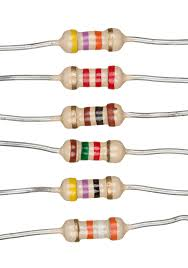
\includegraphics[width=0.6\textwidth]{resistor}
    % Diagram showing the symbol and internal structure of a resistor
    \caption{Symbol and structure of a resistor}
    \label{fig:resistor}
\end{figure}

\begin{figure}[h!]
    \centering
    % 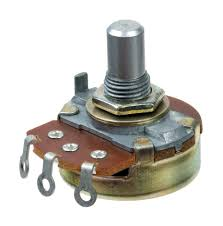
\includegraphics[width=0.6\textwidth]{potentiometer}
    % Diagram showing the symbol and internal structure of a potentiometer
    \caption{Symbol and structure of a potentiometer}
    \label{fig:potentiometer}
\end{figure}

\subsection*{Tables}
\begin{table}[h!]
    \centering
    \caption{Comparison of basic electronic components}
    \label{tab:basic_components}
    \begin{tabular}{|l|l|l|l|}
        \hline
        \textbf{Component} & \textbf{Property} & \textbf{Energy Storage} & \textbf{Common Use} \\
        \hline
        Resistor & Resistance & None & Current limiting, voltage division \\
        Capacitor & Capacitance & Electric field & Energy storage, filtering \\
        Inductor & Inductance & Magnetic field & Energy storage, filtering \\
        \hline
    \end{tabular}
\end{table}

\subsection*{Questions}
\begin{tcolorbox}[colback=gray!10!white,colframe=black!75!black,title={T6A01}]
    What electrical component opposes the flow of current in a DC circuit?
    \begin{enumerate}[label=\Alph*,noitemsep]
        \item Inductor
        \item \textbf{Resistor}
        \item Inverter
        \item Transformer
    \end{enumerate}
\end{tcolorbox}
A resistor opposes the flow of current in a DC circuit, as described by Ohm's Law. Inductors, inverters, and transformers do not primarily oppose current flow in the same way.

%memory_trick T6A01

\begin{tcolorbox}[colback=gray!10!white,colframe=black!75!black,title={T6A02}]
    What type of component is often used as an adjustable volume control?
    \begin{enumerate}[label=\Alph*,noitemsep]
        \item Fixed resistor
        \item Power resistor
        \item \textbf{Potentiometer}
        \item Transformer
    \end{enumerate}
\end{tcolorbox}
A potentiometer is commonly used as an adjustable volume control because it allows for variable resistance, which adjusts the signal level.

%memory_trick T6A02

\begin{tcolorbox}[colback=gray!10!white,colframe=black!75!black,title={T6A03}]
    What electrical parameter is controlled by a potentiometer?
    \begin{enumerate}[label=\Alph*,noitemsep]
        \item Inductance
        \item \textbf{Resistance}
        \item Capacitance
        \item Field strength
    \end{enumerate}
\end{tcolorbox}
A potentiometer controls resistance by adjusting the position of the wiper along the resistive element.

%memory_trick T6A03

\begin{tcolorbox}[colback=gray!10!white,colframe=black!75!black,title={T6A04}]
    What electrical component stores energy in an electric field?
    \begin{enumerate}[label=\Alph*,noitemsep]
        \item Varistor
        \item \textbf{Capacitor}
        \item Inductor
        \item Diode
    \end{enumerate}
\end{tcolorbox}
A capacitor stores energy in an electric field, as opposed to an inductor, which stores energy in a magnetic field.

%memory_trick T6A04

\begin{tcolorbox}[colback=gray!10!white,colframe=black!75!black,title={T6A05}]
    What type of electrical component consists of conductive surfaces separated by an insulator?
    \begin{enumerate}[label=\Alph*,noitemsep]
        \item Resistor
        \item Potentiometer
        \item Oscillator
        \item \textbf{Capacitor}
    \end{enumerate}
\end{tcolorbox}
A capacitor consists of two conductive plates separated by an insulating material (dielectric).

%memory_trick T6A05

\begin{tcolorbox}[colback=gray!10!white,colframe=black!75!black,title={T6A06}]
    What type of electrical component stores energy in a magnetic field?
    \begin{enumerate}[label=\Alph*,noitemsep]
        \item Varistor
        \item Capacitor
        \item \textbf{Inductor}
        \item Diode
    \end{enumerate}
\end{tcolorbox}
An inductor stores energy in a magnetic field, as opposed to a capacitor, which stores energy in an electric field.

%memory_trick T6A06

\begin{tcolorbox}[colback=gray!10!white,colframe=black!75!black,title={T6A07}]
    What electrical component is typically constructed as a coil of wire?
    \begin{enumerate}[label=\Alph*,noitemsep]
        \item Switch
        \item Capacitor
        \item Diode
        \item \textbf{Inductor}
    \end{enumerate}
\end{tcolorbox}
An inductor is typically constructed as a coil of wire, which generates a magnetic field when current flows through it.

%memory_trick T6A07

\begin{tcolorbox}[colback=gray!10!white,colframe=black!75!black,title={T6A08}]
    What is the function of an SPDT switch?
    \begin{enumerate}[label=\Alph*,noitemsep]
        \item A single circuit is opened or closed
        \item Two circuits are opened or closed
        \item \textbf{A single circuit is switched between one of two other circuits}
        \item Two circuits are each switched between one of two other circuits
    \end{enumerate}
\end{tcolorbox}
An SPDT switch connects a single circuit to one of two other circuits, making it useful for routing signals or selecting modes.

%memory_trick T6A08

\subsection*{Summary}
This section covered the basic components used in electronic circuits:
\begin{itemize}
    \item \textbf{Resistors}: Oppose current flow and are used for current limiting and voltage division.
    \item \textbf{Potentiometers}: Adjustable resistors used for volume control and voltage adjustment.
    \item \textbf{Capacitors}: Store energy in an electric field and are used for energy storage and filtering.
    \item \textbf{Inductors}: Store energy in a magnetic field and are used for energy storage and filtering.
    \item \textbf{Switches}: Control the flow of current in circuits, with SPDT switches routing signals between two paths.
\end{itemize}

\section{Semiconductor Components and Their Applications}
\label{section:semiconductor_components}

\subsection*{Forward Voltage Drop in Diodes}
The forward voltage drop in a diode is a critical parameter in circuit design. It refers to the voltage required to allow current to flow through the diode in the forward direction. Different types of diodes exhibit varying forward voltage drops. For example, a silicon diode typically has a forward voltage drop of around 0.7V, while a Schottky diode may have a lower drop of approximately 0.3V. This characteristic is significant because it determines the minimum voltage required for the diode to conduct and influences the efficiency of the circuit.

\subsection*{Transistors as Electronic Switches}
Transistors are versatile semiconductor devices that can function as electronic switches or amplifiers. When used as a switch, a transistor can control the flow of current between its collector and emitter terminals based on the voltage applied to its base terminal. This property makes transistors essential in digital circuits, where they are used to implement logic gates and other switching functions. Additionally, transistors amplify weak signals by controlling a larger current with a smaller input signal, making them indispensable in analog circuits.

\subsection*{Field-Effect Transistors (FETs)}
A Field-Effect Transistor (FET) is a type of transistor that relies on an electric field to control the flow of current. It consists of three terminals: the gate, drain, and source. The gate terminal controls the conductivity between the drain and source by modulating the electric field within the device. FETs are widely used in applications requiring high input impedance and low power consumption, such as in amplifiers and integrated circuits.

\subsection*{Light-Emitting Diodes (LEDs)}
A Light-Emitting Diode (LED) is a semiconductor device that emits light when forward current passes through it. The light emission occurs due to the recombination of electrons and holes within the semiconductor material, releasing energy in the form of photons. LEDs are commonly used in displays, indicators, and lighting due to their efficiency, longevity, and compact size.

\begin{figure}[htbp]
    \centering
    % \includegraphics[width=0.8\textwidth]{diode_structure}
    \caption{Symbol and structure of a diode.}
    \label{fig:diode}
    % Prompt: Diagram showing the symbol and internal structure of a diode.
    % The figure should include the schematic symbol of a diode and a cross-sectional view of its internal structure, highlighting the P-N junction.
\end{figure}

\begin{figure}[htbp]
    \centering
    % \includegraphics[width=0.8\textwidth]{transistor_structure}
    \caption{Symbol and structure of a transistor.}
    \label{fig:transistor}
    % Prompt: Diagram showing the symbol and internal structure of a transistor.
    % The figure should include the schematic symbol of a transistor and a cross-sectional view of its internal structure, showing the emitter, base, and collector regions.
\end{figure}

\begin{table}[htbp]
    \centering
    \caption{Comparison of diode types.}
    \label{tab:diode_types}
    \begin{tabular}{|l|l|l|}
        \hline
        \textbf{Diode Type} & \textbf{Forward Voltage Drop} & \textbf{Applications} \\ \hline
        Silicon Diode       & 0.7V                         & Rectification         \\ \hline
        Schottky Diode      & 0.3V                         & High-speed switching  \\ \hline
        Zener Diode         & Varies                       & Voltage regulation    \\ \hline
    \end{tabular}
    % Prompt: Table comparing different types of diodes and their applications.
\end{table}

\subsection*{Questions}
\begin{tcolorbox}[colback=gray!10!white,colframe=black!75!black,title={T6B01}]
    Which is true about forward voltage drop in a diode?
    \begin{enumerate}[label=\Alph*),noitemsep]
        \item \textbf{It is lower in some diode types than in others}
        \item It is proportional to peak inverse voltage
        \item It indicates that the diode is defective
        \item It has no impact on the voltage delivered to the load
    \end{enumerate}
\end{tcolorbox}
Different diode types, such as silicon and Schottky diodes, have different forward voltage drops. For example, a Schottky diode has a lower forward voltage drop compared to a silicon diode. This characteristic is inherent to the diode's design and does not indicate a defect. The forward voltage drop directly affects the voltage delivered to the load in a circuit. %memory_trick T6B01

\begin{tcolorbox}[colback=gray!10!white,colframe=black!75!black,title={T6B02}]
    What electronic component allows current to flow in only one direction?
    \begin{enumerate}[label=\Alph*),noitemsep]
        \item Resistor
        \item Fuse
        \item \textbf{Diode}
        \item Driven element
    \end{enumerate}
\end{tcolorbox}
A diode is designed to allow current to flow in only one direction, from the anode to the cathode. This property is due to the P-N junction within the diode, which permits current flow in the forward direction while blocking it in the reverse direction. %memory_trick T6B02

\begin{tcolorbox}[colback=gray!10!white,colframe=black!75!black,title={T6B03}]
    Which of these components can be used as an electronic switch?
    \begin{enumerate}[label=\Alph*),noitemsep]
        \item Varistor
        \item Potentiometer
        \item \textbf{Transistor}
        \item Thermistor
    \end{enumerate}
\end{tcolorbox}
A transistor can function as an electronic switch by controlling the flow of current between its collector and emitter terminals based on the voltage applied to its base terminal. This makes it a fundamental component in digital and analog circuits. %memory_trick T6B03

\begin{tcolorbox}[colback=gray!10!white,colframe=black!75!black,title={T6B04}]
    Which of the following components can consist of three regions of semiconductor material?
    \begin{enumerate}[label=\Alph*),noitemsep]
        \item Alternator
        \item \textbf{Transistor}
        \item Triode
        \item Pentagrid converter
    \end{enumerate}
\end{tcolorbox}
A transistor consists of three regions of semiconductor material: the emitter, base, and collector. These regions form the basis of its operation as an amplifier or switch. %memory_trick T6B04

\begin{tcolorbox}[colback=gray!10!white,colframe=black!75!black,title={T6B05}]
    What type of transistor has a gate, drain, and source?
    \begin{enumerate}[label=\Alph*),noitemsep]
        \item Varistor
        \item \textbf{Field-effect}
        \item Tesla-effect
        \item Bipolar junction
    \end{enumerate}
\end{tcolorbox}
A Field-Effect Transistor (FET) has three terminals: the gate, drain, and source. The gate controls the flow of current between the drain and source by modulating the electric field within the device. %memory_trick T6B05

\begin{tcolorbox}[colback=gray!10!white,colframe=black!75!black,title={T6B06}]
    How is the cathode lead of a semiconductor diode often marked on the package?
    \begin{enumerate}[label=\Alph*),noitemsep]
        \item With the word "cathode"
        \item \textbf{With a stripe}
        \item With the letter C
        \item With the letter K
    \end{enumerate}
\end{tcolorbox}
The cathode lead of a semiconductor diode is typically marked with a stripe on the package. This marking helps identify the polarity of the diode during circuit assembly. %memory_trick T6B06

\begin{tcolorbox}[colback=gray!10!white,colframe=black!75!black,title={T6B07}]
    What causes a light-emitting diode (LED) to emit light?
    \begin{enumerate}[label=\Alph*),noitemsep]
        \item \textbf{Forward current}
        \item Reverse current
        \item Capacitively-coupled RF signal
        \item Inductively-coupled RF signal
    \end{enumerate}
\end{tcolorbox}
An LED emits light when forward current passes through it. This current causes electrons and holes to recombine within the semiconductor material, releasing energy in the form of photons. %memory_trick T6B07

\begin{tcolorbox}[colback=gray!10!white,colframe=black!75!black,title={T6B08}]
    What does the abbreviation FET stand for?
    \begin{enumerate}[label=\Alph*),noitemsep]
        \item Frequency Emission Transmitter
        \item Fast Electron Transistor
        \item Free Electron Transmitter
        \item \textbf{Field Effect Transistor}
    \end{enumerate}
\end{tcolorbox}
FET stands for Field-Effect Transistor, a type of transistor that uses an electric field to control the flow of current. %memory_trick T6B08

\subsection*{Summary}
This section covered the fundamental semiconductor components and their applications:
\begin{itemize}
    \item \textbf{Diodes}: Devices that allow current to flow in one direction, with varying forward voltage drops depending on the type.
    \item \textbf{Transistors}: Components that can act as electronic switches or amplifiers, consisting of three semiconductor regions.
    \item \textbf{Field-Effect Transistors (FETs)}: Transistors with gate, drain, and source terminals, used for high input impedance and low power consumption applications.
    \item \textbf{Light-Emitting Diodes (LEDs)}: Diodes that emit light when forward current passes through them, widely used in displays and lighting.
\end{itemize}

\section{Circuit Design and Analysis}
\label{section:circuit_design_and_analysis}

\subsection*{Introduction}
Schematic diagrams are essential tools in circuit design, providing a visual representation of how components are interconnected. They use standardized symbols to represent components, making it easier to understand and analyze circuits. This section will explore the importance of schematic diagrams, how to identify components, and the process of analyzing circuits using these diagrams.

\subsection*{Schematic Diagrams}
Schematic diagrams are the backbone of circuit design. They provide a clear and concise way to represent the connections between components in a circuit. By using standardized symbols, schematic diagrams allow engineers and technicians to quickly understand the structure and function of a circuit. For example, a resistor is represented by a zigzag line, while a transistor is represented by a combination of lines and arrows. These symbols are universally recognized, making schematic diagrams an invaluable tool for communication in the field of electronics.

\subsection*{Component Identification}
Identifying components in a schematic diagram is a fundamental skill in circuit analysis. Each component is represented by a unique symbol, and understanding these symbols is crucial for interpreting the diagram. For instance, a resistor is typically represented by a zigzag line, while a capacitor is represented by two parallel lines. By familiarizing oneself with these symbols, one can quickly identify the components in a circuit and understand their roles. Figure~\ref{fig:schematic_example} provides an example of a schematic diagram with labeled components.

% Example schematic diagram with labeled components
\begin{figure}[h!]
    \centering
    % \includegraphics[width=0.8\textwidth]{schematic_example.svg} % Placeholder for the image
    \caption{Example schematic diagram with labeled components.}
    \label{fig:schematic_example}
\end{figure}

\subsection*{Circuit Analysis}
Analyzing a circuit using a schematic diagram involves identifying the key components and understanding how they interact. This process typically begins with identifying the power sources, such as batteries or power supplies, and then tracing the flow of current through the circuit. By understanding the function of each component, one can predict the behavior of the circuit and diagnose any issues. Table~\ref{tab:schematic_symbols} lists common schematic symbols and their corresponding components, which can be a useful reference during circuit analysis.

% Table listing common schematic symbols and their corresponding components
\begin{table}[h!]
    \centering
    \begin{tabular}{|c|c|}
        \hline
        \textbf{Symbol} & \textbf{Component} \\
        \hline
        \textbackslash zigzag & Resistor \\
        \hline
        \textbackslash parallel lines & Capacitor \\
        \hline
        \textbackslash arrow & Transistor \\
        \hline
        \textbackslash circle & Battery \\
        \hline
    \end{tabular}
    \caption{Common schematic symbols and their corresponding components.}
    \label{tab:schematic_symbols}
\end{table}

\subsection*{Questions}
\begin{tcolorbox}[colback=gray!10!white,colframe=black!75!black,title={T6C01}]
    What is the name of an electrical wiring diagram that uses standard component symbols?
    \begin{enumerate}[label=\Alph*),noitemsep]
        \item Bill of materials
        \item Connector pinout
        \item \textbf{Schematic}
        \item Flow chart
    \end{enumerate}
\end{tcolorbox}
A schematic diagram is the correct term for an electrical wiring diagram that uses standard component symbols. It is a visual representation of the circuit, showing how components are connected.

%memory_trick T6C01

\begin{tcolorbox}[colback=gray!10!white,colframe=black!75!black,title={T6C02}]
    What is component 1 in figure T-1?
    \begin{enumerate}[label=\Alph*),noitemsep]
        \item \textbf{Resistor}
        \item Transistor
        \item Battery
        \item Connector
    \end{enumerate}
\end{tcolorbox}
Component 1 in figure T-1 is a resistor. Resistors are commonly represented by a zigzag line in schematic diagrams.

%memory_trick T6C02

\begin{tcolorbox}[colback=gray!10!white,colframe=black!75!black,title={T6C03}]
    What is component 2 in figure T-1?
    \begin{enumerate}[label=\Alph*),noitemsep]
        \item Resistor
        \item \textbf{Transistor}
        \item Indicator lamp
        \item Connector
    \end{enumerate}
\end{tcolorbox}
Component 2 in figure T-1 is a transistor. Transistors are typically represented by a combination of lines and arrows in schematic diagrams.

%memory_trick T6C03

\begin{tcolorbox}[colback=gray!10!white,colframe=black!75!black,title={T6C04}]
    What is component 3 in figure T-1?
    \begin{enumerate}[label=\Alph*),noitemsep]
        \item Resistor
        \item Transistor
        \item \textbf{Lamp}
        \item Ground symbol
    \end{enumerate}
\end{tcolorbox}
Component 3 in figure T-1 is a lamp. Lamps are often represented by a circle with a cross inside in schematic diagrams.

%memory_trick T6C04

\begin{tcolorbox}[colback=gray!10!white,colframe=black!75!black,title={T6C05}]
    What is component 4 in figure T-1?
    \begin{enumerate}[label=\Alph*),noitemsep]
        \item Resistor
        \item Transistor
        \item Ground symbol
        \item \textbf{Battery}
    \end{enumerate}
\end{tcolorbox}
Component 4 in figure T-1 is a battery. Batteries are typically represented by a pair of parallel lines, one longer than the other, in schematic diagrams.

%memory_trick T6C05

\begin{tcolorbox}[colback=gray!10!white,colframe=black!75!black,title={T6C06}]
    What is component 6 in figure T-2?
    \begin{enumerate}[label=\Alph*),noitemsep]
        \item Resistor
        \item \textbf{Capacitor}
        \item Regulator IC
        \item Transistor
    \end{enumerate}
\end{tcolorbox}
Component 6 in figure T-2 is a capacitor. Capacitors are typically represented by two parallel lines in schematic diagrams.

%memory_trick T6C06

\begin{tcolorbox}[colback=gray!10!white,colframe=black!75!black,title={T6C07}]
    What is component 8 in figure T-2?
    \begin{enumerate}[label=\Alph*),noitemsep]
        \item Resistor
        \item Inductor
        \item Regulator IC
        \item \textbf{Light emitting diode}
    \end{enumerate}
\end{tcolorbox}
Component 8 in figure T-2 is a light emitting diode (LED). LEDs are typically represented by a triangle with a line pointing outward and a small arrow indicating light emission.

%memory_trick T6C07

\begin{tcolorbox}[colback=gray!10!white,colframe=black!75!black,title={T6C08}]
    What is component 9 in figure T-2?
    \begin{enumerate}[label=\Alph*),noitemsep]
        \item Variable capacitor
        \item Variable inductor
        \item \textbf{Variable resistor}
        \item Variable transformer
    \end{enumerate}
\end{tcolorbox}
Component 9 in figure T-2 is a variable resistor. Variable resistors are typically represented by a zigzag line with an arrow pointing to it, indicating adjustability.

%memory_trick T6C08

\subsection*{Summary}
This section covered the importance of schematic diagrams in circuit design, the identification of components, and the process of analyzing circuits. Key concepts include:

\begin{itemize}
    \item \textbf{Schematic Diagrams}: Visual representations of circuits using standardized symbols.
    \item \textbf{Component Identification}: Recognizing components by their symbols in schematic diagrams.
    \item \textbf{Circuit Analysis}: Understanding the function and interaction of components in a circuit.
\end{itemize}

By mastering these concepts, one can effectively design and analyze electronic circuits.

\section{Advanced Electronics and Core Technologies}
\label{section:advanced_electronics}

\subsection*{Rectifiers}
A rectifier is an electronic device that converts alternating current (AC) into direct current (DC). This is achieved by allowing current to flow in only one direction, effectively "rectifying" the AC signal. Rectifiers are commonly used in power supplies to provide a stable DC voltage for electronic devices. The simplest form of a rectifier is the diode, which allows current to pass in one direction while blocking it in the opposite direction. More complex rectifier circuits, such as the full-wave bridge rectifier, are used to improve efficiency and reduce ripple in the output DC signal.

\begin{figure}[h!]
    \centering
    % \includegraphics[width=0.8\textwidth]{rectifier_circuit_operation}
    \caption{Rectifier circuit operation. The diagram should show the input AC waveform, the rectifier diodes, and the resulting DC waveform with ripple.}
    \label{fig:rectifier}
\end{figure}

\subsection*{Relays}
A relay is an electrically-controlled switch that uses a small electrical signal to control a larger current or voltage. Relays are commonly used in applications where it is necessary to control a high-power circuit with a low-power signal, such as in automotive systems or industrial control systems. The basic operation of a relay involves an electromagnet that, when energized, moves a set of contacts to either open or close a circuit.

\begin{figure}[h!]
    \centering
    % \includegraphics[width=0.8\textwidth]{relay_structure_operation}
    \caption{Relay structure and operation. The diagram should show the electromagnet, the movable armature, and the contacts in both the open and closed positions.}
    \label{fig:relay}
\end{figure}

\subsection*{Shielded Wire}
Shielded wire is used to prevent the coupling of unwanted signals to or from the wire. This is particularly important in environments where electromagnetic interference (EMI) is a concern, such as in radio frequency (RF) circuits or in data transmission lines. The shield, typically made of a conductive material like copper, surrounds the inner conductor and is grounded to absorb or reflect any interfering signals.

\subsection*{Regulators}
A voltage regulator is a circuit that maintains a constant output voltage regardless of changes in input voltage or load conditions. This is essential in power supplies to ensure that electronic devices receive a stable voltage, which is critical for their proper operation. There are several types of voltage regulators, including linear regulators and switching regulators, each with its own advantages and disadvantages.

\begin{table}[h!]
    \centering
    \begin{tabular}{|l|l|l|}
        \hline
        \textbf{Type} & \textbf{Advantages} & \textbf{Applications} \\
        \hline
        Linear Regulator & Simple, low noise & Low-power devices \\
        Switching Regulator & High efficiency, compact & High-power devices \\
        \hline
    \end{tabular}
    \caption{Comparison of voltage regulators.}
    \label{tab:regulators}
\end{table}

\subsection*{Questions}

\begin{tcolorbox}[colback=gray!10!white,colframe=black!75!black,title={T6D01}]
    Which of the following devices or circuits changes an alternating current into a varying direct current signal?
    \begin{enumerate}[label=\Alph*),noitemsep]
        \item Transformer
        \item \textbf{Rectifier}
        \item Amplifier
        \item Reflector
    \end{enumerate}
\end{tcolorbox}
A rectifier is specifically designed to convert AC to DC by allowing current to flow in only one direction. Transformers change voltage levels, amplifiers increase signal strength, and reflectors are not related to electrical signal conversion.

%memory_trick T6D01

\begin{tcolorbox}[colback=gray!10!white,colframe=black!75!black,title={T6D02}]
    What is a relay?
    \begin{enumerate}[label=\Alph*),noitemsep]
        \item \textbf{An electrically-controlled switch}
        \item A current controlled amplifier
        \item An inverting amplifier
        \item A pass transistor
    \end{enumerate}
\end{tcolorbox}
A relay is an electrically-controlled switch that uses a small electrical signal to control a larger current or voltage. It is not an amplifier or a transistor.

%memory_trick T6D02

\begin{tcolorbox}[colback=gray!10!white,colframe=black!75!black,title={T6D03}]
    Which of the following is a reason to use shielded wire?
    \begin{enumerate}[label=\Alph*),noitemsep]
        \item To decrease the resistance of DC power connections
        \item To increase the current carrying capability of the wire
        \item \textbf{To prevent coupling of unwanted signals to or from the wire}
        \item To couple the wire to other signals
    \end{enumerate}
\end{tcolorbox}
Shielded wire is used to prevent electromagnetic interference (EMI) from affecting the signal carried by the wire. It does not decrease resistance or increase current capacity.

%memory_trick T6D03

\begin{tcolorbox}[colback=gray!10!white,colframe=black!75!black,title={T6D04}]
    Which of the following displays an electrical quantity as a numeric value?
    \begin{enumerate}[label=\Alph*),noitemsep]
        \item Potentiometer
        \item Transistor
        \item \textbf{Meter}
        \item Relay
    \end{enumerate}
\end{tcolorbox}
A meter is designed to display electrical quantities such as voltage, current, or resistance as numeric values. Potentiometers, transistors, and relays do not display values.

%memory_trick T6D04

\begin{tcolorbox}[colback=gray!10!white,colframe=black!75!black,title={T6D05}]
    What type of circuit controls the amount of voltage from a power supply?
    \begin{enumerate}[label=\Alph*),noitemsep]
        \item \textbf{Regulator}
        \item Oscillator
        \item Filter
        \item Phase inverter
    \end{enumerate}
\end{tcolorbox}
A voltage regulator maintains a constant output voltage regardless of changes in input voltage or load conditions. Oscillators, filters, and phase inverters do not control voltage levels.

%memory_trick T6D05

\begin{tcolorbox}[colback=gray!10!white,colframe=black!75!black,title={T6D06}]
    What component changes 120 V AC power to a lower AC voltage for other uses?
    \begin{enumerate}[label=\Alph*),noitemsep]
        \item Variable capacitor
        \item \textbf{Transformer}
        \item Transistor
        \item Diode
    \end{enumerate}
\end{tcolorbox}
A transformer is used to step down (or step up) AC voltage levels. Variable capacitors, transistors, and diodes do not change AC voltage levels.

%memory_trick T6D06

\begin{tcolorbox}[colback=gray!10!white,colframe=black!75!black,title={T6D07}]
    Which of the following is commonly used as a visual indicator?
    \begin{enumerate}[label=\Alph*),noitemsep]
        \item \textbf{LED}
        \item FET
        \item Zener diode
        \item Bipolar transistor
    \end{enumerate}
\end{tcolorbox}
An LED (Light Emitting Diode) is commonly used as a visual indicator due to its ability to emit light when current passes through it. FETs, Zener diodes, and bipolar transistors are not used for visual indication.

%memory_trick T6D07

\begin{tcolorbox}[colback=gray!10!white,colframe=black!75!black,title={T6D08}]
    Which of the following is combined with an inductor to make a resonant circuit?
    \begin{enumerate}[label=\Alph*),noitemsep]
        \item Resistor
        \item Zener diode
        \item Potentiometer
        \item \textbf{Capacitor}
    \end{enumerate}
\end{tcolorbox}
A capacitor, when combined with an inductor, forms a resonant circuit that can oscillate at a specific frequency. Resistors, Zener diodes, and potentiometers do not form resonant circuits with inductors.

%memory_trick T6D08

\subsection*{Summary}
This section covered several key concepts in advanced electronics:
\begin{itemize}
    \item \textbf{Rectifiers}: Devices that convert AC to DC, essential in power supplies.
    \item \textbf{Relays}: Electrically-controlled switches used to manage high-power circuits with low-power signals.
    \item \textbf{Shielded Wire}: Used to prevent electromagnetic interference in sensitive circuits.
    \item \textbf{Regulators}: Circuits that maintain a constant output voltage, crucial for stable power supply.
    \item \textbf{Resonant Circuits}: Circuits that combine inductors and capacitors to oscillate at specific frequencies, used in tuning and filtering applications.
\end{itemize}

\chapter{PRACTICAL CIRCUITS}
\label{chapter:practical_circuits}
\section{Signal Essentials}
\label{section:signal_essentials}

\subsection*{Receiver Sensitivity}
Receiver sensitivity refers to the ability of a receiver to detect weak signals. It is a critical parameter in radio communication, as it determines the minimum signal strength that can be reliably detected. High sensitivity allows a receiver to pick up distant or weak signals, which is essential for effective communication, especially in low-power or long-distance scenarios.

\subsection*{Transceiver Functionality}
A transceiver is a device that combines both a transmitter and a receiver in a single unit. It allows for two-way communication by enabling the transmission and reception of signals. Key components of a transceiver include the transmitter, receiver, and often a mixer for frequency conversion. Figure~\ref{fig:transceiver_block_diagram} illustrates the block diagram of a basic transceiver.

\begin{figure}[h!]
    \centering
    % \includegraphics[width=0.8\textwidth]{transceiver_block_diagram.svg}
    \caption{Block diagram of a basic transceiver showing key components.}
    \label{fig:transceiver_block_diagram}
    % Prompt: Diagram of a basic transceiver block diagram
    % The figure should include blocks for the transmitter, receiver, mixer, and antenna.
\end{figure}

\subsection*{Frequency Conversion}
Frequency conversion is the process of changing a signal from one frequency to another. This is typically achieved using a mixer, which combines the input signal with a local oscillator signal to produce sum and difference frequencies. The desired frequency is then filtered out. Figure~\ref{fig:frequency_conversion} demonstrates this process.

\begin{figure}[h!]
    \centering
    % \includegraphics[width=0.8\textwidth]{frequency_conversion.svg}
    \caption{Frequency conversion process using a mixer.}
    \label{fig:frequency_conversion}
    % Prompt: Illustration of frequency conversion using a mixer
    % The figure should show the input signal, local oscillator, mixer, and output signal.
\end{figure}

\subsection*{Signal Discrimination}
Selectivity is the ability of a receiver to discriminate between multiple signals, particularly those that are close in frequency. High selectivity ensures that the receiver can isolate the desired signal from unwanted interference, which is crucial for clear communication.

\subsection*{Oscillator Circuits}
An oscillator is a circuit that generates a signal at a specific frequency. It is a fundamental component in both transmitters and receivers, providing the carrier signal for modulation and the local oscillator signal for frequency conversion.

\subsection*{Transverter Usage}
A transverter is a device that converts the RF input and output of a transceiver to another frequency band. This allows the transceiver to operate on bands for which it was not originally designed, extending its versatility.

\subsection*{PTT Input Function}
The PTT (Push-To-Talk) input on a transceiver is used to switch the device from receive mode to transmit mode when grounded. This is essential for half-duplex communication, where the same frequency is used for both transmission and reception.

\subsection*{Modulation Techniques}
Modulation is the process of combining speech or data with an RF carrier signal. This allows the information to be transmitted over long distances. Common modulation techniques include AM (Amplitude Modulation), FM (Frequency Modulation), and SSB (Single Sideband). Table~\ref{tab:modulation_comparison} provides a comparison of these techniques.

\begin{table}[h!]
    \centering
    \begin{tabular}{|l|l|l|l|}
        \hline
        \textbf{Modulation Type} & \textbf{Bandwidth} & \textbf{Efficiency} & \textbf{Complexity} \\
        \hline
        AM & High & Low & Low \\
        FM & Medium & Medium & Medium \\
        SSB & Low & High & High \\
        \hline
    \end{tabular}
    \caption{Comparison of AM, FM, and SSB modulation techniques.}
    \label{tab:modulation_comparison}
    % Prompt: Comparison of different modulation techniques
\end{table}

\subsection*{Questions}
\begin{tcolorbox}[colback=gray!10!white,colframe=black!75!black,title={T7A01}]
    Which term describes the ability of a receiver to detect the presence of a signal?
    \begin{enumerate}[label=\Alph*,noitemsep]
        \item Linearity
        \item \textbf{Sensitivity}
        \item Selectivity
        \item Total Harmonic Distortion
    \end{enumerate}
\end{tcolorbox}
Sensitivity is the correct term, as it directly relates to the receiver's ability to detect weak signals. Linearity refers to the proportionality of input and output, selectivity refers to the ability to discriminate between signals, and total harmonic distortion is a measure of signal distortion.

%memory_trick T7A01

\begin{tcolorbox}[colback=gray!10!white,colframe=black!75!black,title={T7A02}]
    What is a transceiver?
    \begin{enumerate}[label=\Alph*,noitemsep]
        \item \textbf{A device that combines a receiver and transmitter}
        \item A device for matching feed line impedance to 50 ohms
        \item A device for automatically sending and decoding Morse code
        \item A device for converting receiver and transmitter frequencies to another band
    \end{enumerate}
\end{tcolorbox}
A transceiver integrates both a transmitter and a receiver, enabling two-way communication. The other options describe different devices or functions, such as impedance matching or frequency conversion.

%memory_trick T7A02

\begin{tcolorbox}[colback=gray!10!white,colframe=black!75!black,title={T7A03}]
    Which of the following is used to convert a signal from one frequency to another?
    \begin{enumerate}[label=\Alph*,noitemsep]
        \item Phase splitter
        \item \textbf{Mixer}
        \item Inverter
        \item Amplifier
    \end{enumerate}
\end{tcolorbox}
A mixer is used for frequency conversion by combining the input signal with a local oscillator signal. Phase splitters, inverters, and amplifiers serve different purposes in signal processing.

%memory_trick T7A03

\begin{tcolorbox}[colback=gray!10!white,colframe=black!75!black,title={T7A04}]
    Which term describes the ability of a receiver to discriminate between multiple signals?
    \begin{enumerate}[label=\Alph*,noitemsep]
        \item Discrimination ratio
        \item Sensitivity
        \item \textbf{Selectivity}
        \item Harmonic distortion
    \end{enumerate}
\end{tcolorbox}
Selectivity is the correct term, as it refers to the receiver's ability to distinguish between signals close in frequency. Sensitivity relates to detecting weak signals, while harmonic distortion is a measure of signal quality.

%memory_trick T7A04

\begin{tcolorbox}[colback=gray!10!white,colframe=black!75!black,title={T7A05}]
    What is the name of a circuit that generates a signal at a specific frequency?
    \begin{enumerate}[label=\Alph*,noitemsep]
        \item Reactance modulator
        \item Phase modulator
        \item Low-pass filter
        \item \textbf{Oscillator}
    \end{enumerate}
\end{tcolorbox}
An oscillator generates a signal at a specific frequency, making it essential for both transmitters and receivers. Reactance modulators, phase modulators, and low-pass filters serve different functions in signal processing.

%memory_trick T7A05

\begin{tcolorbox}[colback=gray!10!white,colframe=black!75!black,title={T7A06}]
    What device converts the RF input and output of a transceiver to another band?
    \begin{enumerate}[label=\Alph*,noitemsep]
        \item High-pass filter
        \item Low-pass filter
        \item \textbf{Transverter}
        \item Phase converter
    \end{enumerate}
\end{tcolorbox}
A transverter is used to convert the RF input and output of a transceiver to another frequency band, allowing operation on different bands. High-pass and low-pass filters are used for signal filtering, while a phase converter changes the phase of a signal.

%memory_trick T7A06

\begin{tcolorbox}[colback=gray!10!white,colframe=black!75!black,title={T7A07}]
    What is the function of a transceiver’s PTT input?
    \begin{enumerate}[label=\Alph*,noitemsep]
        \item Input for a key used to send CW
        \item \textbf{Switches transceiver from receive to transmit when grounded}
        \item Provides a transmit tuning tone when grounded
        \item Input for a preamplifier tuning tone
    \end{enumerate}
\end{tcolorbox}
The PTT input switches the transceiver from receive to transmit mode when grounded, enabling half-duplex communication. The other options describe different functions not related to the PTT input.

%memory_trick T7A07

\begin{tcolorbox}[colback=gray!10!white,colframe=black!75!black,title={T7A08}]
    Which of the following describes combining speech with an RF carrier signal?
    \begin{enumerate}[label=\Alph*,noitemsep]
        \item Impedance matching
        \item Oscillation
        \item \textbf{Modulation}
        \item Low-pass filtering
    \end{enumerate}
\end{tcolorbox}
Modulation is the process of combining speech or data with an RF carrier signal, enabling the transmission of information. Impedance matching, oscillation, and low-pass filtering are unrelated to this process.

%memory_trick T7A08

\subsection*{Summary}
This section covered essential concepts in radio communication, including:
\begin{itemize}
    \item \textbf{Receiver Sensitivity}: The ability to detect weak signals.
    \item \textbf{Transceiver Functionality}: A device combining a transmitter and receiver.
    \item \textbf{Frequency Conversion}: The process of changing signal frequency using a mixer.
    \item \textbf{Signal Discrimination}: The ability to distinguish between signals close in frequency.
    \item \textbf{Oscillator Circuits}: Circuits that generate specific frequencies.
    \item \textbf{Transverter Usage}: Devices that convert RF signals to another band.
    \item \textbf{PTT Input Function}: Switches a transceiver from receive to transmit mode.
    \item \textbf{Modulation Techniques}: Methods for combining speech or data with an RF carrier.
\end{itemize}

\section{Radio Troubleshooting Essentials}
\label{section:radio_troubleshooting}

\subsection*{Over-deviation in FM Transceivers}
Over-deviation in FM transceivers occurs when the frequency deviation exceeds the allowed limits, causing distortion and potential interference with adjacent channels. This can be addressed by adjusting the microphone gain or speaking farther away from the microphone to reduce the input signal level.

\subsection*{RF Interference}
RF interference in broadcast receivers is often caused by strong signals outside the AM or FM band that the receiver cannot reject. This can lead to unintentional reception of amateur radio transmissions. Proper filtering and shielding can mitigate this issue.

\subsection*{Harmonics and Spurious Emissions}
Harmonics and spurious emissions are unwanted signals generated by transmitters that can cause interference. These signals are often multiples of the fundamental frequency and can be reduced by using filters and ensuring proper transmitter operation.

\subsection*{RF Feedback}
RF feedback occurs when RF current flows on the shield of a microphone cable, causing distorted audio. This can be mitigated by using ferrite chokes, which absorb the RF energy and prevent it from affecting the audio signal.

\subsection*{Band-reject Filters}
Band-reject filters are used to block specific frequencies that cause interference. For example, they can be installed at the antenna input of a receiver to block strong amateur signals that cause fundamental overload.

\subsection*{Interference Resolution}
When a neighbor reports interference from your amateur station, the first step is to ensure your station is functioning properly and not causing interference to your own equipment. If the issue persists, work with your neighbor to identify and resolve the problem.

\subsection*{Cable TV Interference}
Cable TV interference caused by amateur radio transmissions can be resolved by ensuring your station meets good amateur practice standards and using appropriate filters to block interfering signals.

\begin{figure}[h!]
    \centering
    %\includegraphics[width=0.8\textwidth]{rf_interference}
    \caption{Illustration of RF interference paths and mitigation techniques.}
    \label{fig:rf_interference}
    % Prompt: Diagram showing RF interference paths
\end{figure}

\begin{figure}[h!]
    \centering
    %\includegraphics[width=0.8\textwidth]{ferrite_choke}
    \caption{Ferrite choke installed on a cable to reduce RF feedback.}
    \label{fig:ferrite_choke}
    % Prompt: Illustration of a ferrite choke on a cable
\end{figure}

\begin{table}[h!]
    \centering
    \begin{tabular}{|l|l|}
        \hline
        \textbf{Interference Source} & \textbf{Solution} \\
        \hline
        Over-deviation in FM transceivers & Adjust microphone gain or distance \\
        RF interference in broadcast receivers & Use filters and shielding \\
        Harmonics and spurious emissions & Use filters and ensure proper transmitter operation \\
        RF feedback & Install ferrite chokes \\
        Fundamental overload & Use band-reject filters \\
        \hline
    \end{tabular}
    \caption{Table listing common RF interference sources and their solutions.}
    \label{tab:rf_interference_solutions}
\end{table}

\subsection*{Questions}
\begin{tcolorbox}[colback=gray!10!white,colframe=black!75!black,title={T7B01}]
    What can you do if you are told your FM handheld or mobile transceiver is over-deviating?
    \begin{enumerate}[label=\Alph*,noitemsep]
        \item Talk louder into the microphone
        \item Let the transceiver cool off
        \item Change to a higher power level
        \item \textbf{Talk farther away from the microphone}
    \end{enumerate}
\end{tcolorbox}
Over-deviation occurs when the input signal is too strong, causing excessive frequency deviation. Speaking farther from the microphone reduces the input level, addressing the issue. Other options do not directly address the root cause.

%memory_trick T7B01

\begin{tcolorbox}[colback=gray!10!white,colframe=black!75!black,title={T7B02}]
    What would cause a broadcast AM or FM radio to receive an amateur radio transmission unintentionally?
    \begin{enumerate}[label=\Alph*,noitemsep]
        \item \textbf{The receiver is unable to reject strong signals outside the AM or FM band}
        \item The microphone gain of the transmitter is turned up too high
        \item The audio amplifier of the transmitter is overloaded
        \item The deviation of an FM transmitter is set too low
    \end{enumerate}
\end{tcolorbox}
Broadcast receivers may lack the filtering to reject strong signals outside their intended band, leading to unintentional reception of amateur transmissions. The other options are unrelated to this issue.

%memory_trick T7B02

\begin{tcolorbox}[colback=gray!10!white,colframe=black!75!black,title={T7B03}]
    Which of the following can cause radio frequency interference?
    \begin{enumerate}[label=\Alph*,noitemsep]
        \item Fundamental overload
        \item Harmonics
        \item Spurious emissions
        \item \textbf{All these choices are correct}
    \end{enumerate}
\end{tcolorbox}
Fundamental overload, harmonics, and spurious emissions are all potential sources of RF interference. Each can disrupt communication if not properly managed.

%memory_trick T7B03

\begin{tcolorbox}[colback=gray!10!white,colframe=black!75!black,title={T7B04}]
    Which of the following could you use to cure distorted audio caused by RF current on the shield of a microphone cable?
    \begin{enumerate}[label=\Alph*,noitemsep]
        \item Band-pass filter
        \item Low-pass filter
        \item Preamplifier
        \item \textbf{Ferrite choke}
    \end{enumerate}
\end{tcolorbox}
Ferrite chokes absorb RF energy on the cable shield, preventing it from causing audio distortion. Filters and preamplifiers do not address this specific issue.

%memory_trick T7B04

\begin{tcolorbox}[colback=gray!10!white,colframe=black!75!black,title={T7B05}]
    How can fundamental overload of a non-amateur radio or TV receiver by an amateur signal be reduced or eliminated?
    \begin{enumerate}[label=\Alph*,noitemsep]
        \item \textbf{Block the amateur signal with a filter at the antenna input of the affected receiver}
        \item Block the interfering signal with a filter on the amateur transmitter
        \item Switch the transmitter from FM to SSB
        \item Switch the transmitter to a narrow-band mode
    \end{enumerate}
\end{tcolorbox}
Installing a filter at the receiver's antenna input blocks the interfering amateur signal. Filters on the transmitter or mode changes do not directly address receiver overload.

%memory_trick T7B05

\begin{tcolorbox}[colback=gray!10!white,colframe=black!75!black,title={T7B06}]
    Which of the following actions should you take if a neighbor tells you that your station’s transmissions are interfering with their radio or TV reception?
    \begin{enumerate}[label=\Alph*,noitemsep]
        \item \textbf{Make sure that your station is functioning properly and that it does not cause interference to your own radio or television when it is tuned to the same channel}
        \item Immediately turn off your transmitter and contact the nearest FCC office for assistance
        \item Install a harmonic doubler on the output of your transmitter and tune it until the interference is eliminated
        \item All these choices are correct
    \end{enumerate}
\end{tcolorbox}
The first step is to verify your station's operation and ensure it is not causing interference to your own equipment. This helps identify if the issue is with your station or the neighbor's equipment.

%memory_trick T7B06

\begin{tcolorbox}[colback=gray!10!white,colframe=black!75!black,title={T7B07}]
    Which of the following can reduce overload of a VHF transceiver by a nearby commercial FM station?
    \begin{enumerate}[label=\Alph*,noitemsep]
        \item Installing an RF preamplifier
        \item Using double-shielded coaxial cable
        \item Installing bypass capacitors on the microphone cable
        \item \textbf{Installing a band-reject filter}
    \end{enumerate}
\end{tcolorbox}
A band-reject filter blocks the specific frequency of the commercial FM station, reducing overload. Preamplifiers and shielding do not address this issue.

%memory_trick T7B07

\begin{tcolorbox}[colback=gray!10!white,colframe=black!75!black,title={T7B08}]
    What should you do if something in a neighbor’s home is causing harmful interference to your amateur station?
    \begin{enumerate}[label=\Alph*,noitemsep]
        \item Work with your neighbor to identify the offending device
        \item Politely inform your neighbor that FCC rules prohibit the use of devices that cause interference
        \item Make sure your station meets the standards of good amateur practice
        \item \textbf{All these choices are correct}
    \end{enumerate}
\end{tcolorbox}
All the listed actions are appropriate steps to resolve interference caused by a neighbor's device. Cooperation and adherence to FCC rules are key.

%memory_trick T7B08

\subsection*{Summary}
\begin{itemize}
    \item \textbf{Over-deviation in FM Transceivers}: Adjust microphone gain or distance to reduce input signal level.
    \item \textbf{RF Interference}: Caused by strong signals outside the intended band; mitigated with filters and shielding.
    \item \textbf{Harmonics and Spurious Emissions}: Unwanted signals that cause interference; reduced with proper filtering.
    \item \textbf{RF Feedback}: Distorted audio caused by RF current on microphone cables; mitigated with ferrite chokes.
    \item \textbf{Band-reject Filters}: Block specific frequencies to reduce interference.
    \item \textbf{Interference Resolution}: Verify station operation and work with neighbors to resolve issues.
    \item \textbf{Cable TV Interference}: Ensure proper station operation and use filters to block interfering signals.
\end{itemize}

\section{Test Equipment and Antenna Basics}
\label{section:test_equipment_antenna_basics}

\subsection*{Purpose and Construction of a Dummy Load}
A dummy load is a device used to simulate an antenna's electrical characteristics without radiating radio frequency (RF) energy. It is primarily used to prevent transmitting signals over the air when testing or tuning a transmitter. A dummy load typically consists of a non-inductive resistor mounted on a heat sink to dissipate the power as heat. This ensures that the transmitter can be tested safely without causing interference.

\subsection*{Antenna Resonance and Antenna Analyzers}
An antenna analyzer is a crucial tool for determining if an antenna is resonant at the desired operating frequency. Resonance occurs when the antenna's impedance is purely resistive, minimizing the standing wave ratio (SWR). By measuring the impedance and SWR, an antenna analyzer helps ensure optimal performance and efficiency of the antenna system.

\subsection*{Standing Wave Ratio (SWR) and Impedance Matching}
SWR is a measure of how well the antenna's impedance matches the feed line's impedance. A perfect match is indicated by an SWR of 1:1, meaning all the power is transferred to the antenna without reflection. High SWR values indicate impedance mismatch, which can lead to power loss, heat generation, and potential damage to the transmitter. Impedance matching is critical for maximizing power transfer and minimizing reflections.

\subsection*{Coaxial Cable Issues and Prevention}
Coaxial cables are prone to failure due to factors such as moisture ingress, UV degradation, and physical damage. Moisture in the cable can cause signal loss and corrosion, while UV exposure can degrade the outer jacket. Using UV-resistant jackets and proper sealing techniques can mitigate these issues. Regular inspection and maintenance are also essential to ensure the longevity of coaxial cables.

\subsection*{Directional Wattmeters and SWR Measurement}
Directional wattmeters are used to measure SWR by comparing the forward and reflected power in a transmission line. These instruments provide valuable information about the efficiency of the antenna system and help identify impedance mismatches. A high SWR reading, such as 4:1, indicates a significant impedance mismatch, which can lead to power loss and potential damage to the transmitter.

\subsection*{Heat Dissipation in Dummy Loads and Feed Lines}
Power lost in a feed line is converted into heat, which can cause the cable to degrade over time. Similarly, dummy loads dissipate the transmitter's power as heat, requiring robust heat sinks to prevent overheating. Proper heat management is essential to maintain the performance and reliability of both dummy loads and feed lines.

\begin{figure}[h]
    \centering
    % \includegraphics[width=0.8\textwidth]{dummy_load.svg}
    \caption{Dummy load connected to a transmitter for testing purposes.}
    \label{fig:dummy_load}
    % Prompt: Diagram of a dummy load connected to a transmitter. The diagram should show the transmitter, the dummy load, and the heat sink.
\end{figure}

\begin{figure}[h]
    \centering
    % \includegraphics[width=0.8\textwidth]{swr_measurement.svg}
    \caption{Measurement of SWR using a directional wattmeter.}
    \label{fig:swr_measurement}
    % Prompt: Illustration of SWR measurement using a directional wattmeter. The figure should show the transmitter, the feed line, the directional wattmeter, and the antenna.
\end{figure}

\begin{table}[h]
    \centering
    \caption{Comparison of different types of coaxial cables.}
    \label{tab:coaxial_cable_comparison}
    \begin{tabular}{|l|c|c|c|}
        \hline
        \textbf{Type} & \textbf{Air Core} & \textbf{Foam} & \textbf{Solid Dielectric} \\
        \hline
        Impedance & 50-75 $\Omega$ & 50-75 $\Omega$ & 50-75 $\Omega$ \\
        Loss & Low & Medium & High \\
        Flexibility & High & Medium & Low \\
        Cost & High & Medium & Low \\
        \hline
    \end{tabular}
    % Prompt: Table comparing air core, foam, and solid dielectric coaxial cables. Include columns for impedance, loss, flexibility, and cost.
\end{table}

\subsection*{Questions}
\begin{tcolorbox}[colback=gray!10!white,colframe=black!75!black,title={T7C01}]
    What is the primary purpose of a dummy load?
    \begin{enumerate}[label=\Alph*),noitemsep]
        \item \textbf{To prevent transmitting signals over the air when making tests}
        \item To prevent over-modulation of a transmitter
        \item To improve the efficiency of an antenna
        \item To improve the signal-to-noise ratio of a receiver
    \end{enumerate}
\end{tcolorbox}
A dummy load is used to absorb the transmitter's power without radiating it, allowing safe testing and tuning. The other options are incorrect because a dummy load does not affect modulation, antenna efficiency, or signal-to-noise ratio.

%memory_trick T7C01

\begin{tcolorbox}[colback=gray!10!white,colframe=black!75!black,title={T7C02}]
    Which of the following is used to determine if an antenna is resonant at the desired operating frequency?
    \begin{enumerate}[label=\Alph*),noitemsep]
        \item A VTVM
        \item \textbf{An antenna analyzer}
        \item A Q meter
        \item A frequency counter
    \end{enumerate}
\end{tcolorbox}
An antenna analyzer measures impedance and SWR to determine resonance. A VTVM measures voltage, a Q meter measures quality factor, and a frequency counter measures frequency, none of which directly indicate resonance.

%memory_trick T7C02

\begin{tcolorbox}[colback=gray!10!white,colframe=black!75!black,title={T7C03}]
    What does a dummy load consist of?
    \begin{enumerate}[label=\Alph*),noitemsep]
        \item A high-gain amplifier and a TR switch
        \item \textbf{A non-inductive resistor mounted on a heat sink}
        \item A low-voltage power supply and a DC relay
        \item A 50-ohm reactance used to terminate a transmission line
    \end{enumerate}
\end{tcolorbox}
A dummy load is a non-inductive resistor that dissipates power as heat. The other options describe components unrelated to dummy loads.

%memory_trick T7C03

\subsection*{Summary}
This section covered the basics of test equipment and antennas, including the purpose and construction of dummy loads, the use of antenna analyzers, and the importance of SWR and impedance matching. Key concepts include:
\begin{itemize}
    \item \textbf{Dummy Loads}: Non-inductive resistors used to absorb transmitter power during testing.
    \item \textbf{Antenna Resonance}: Achieved when the antenna's impedance is purely resistive, minimizing SWR.
    \item \textbf{SWR Measurement}: Indicates the efficiency of power transfer between the feed line and antenna.
    \item \textbf{Impedance Matching}: Ensures maximum power transfer and minimizes reflections.
    \item \textbf{Coaxial Cable Issues}: Moisture, UV degradation, and physical damage can lead to cable failure.
    \item \textbf{Heat Dissipation}: Power lost in feed lines and dummy loads is converted into heat.
    \item \textbf{Directional Wattmeters}: Used to measure SWR by comparing forward and reflected power.
    \item \textbf{Moisture in Cables}: Can cause signal loss and corrosion, mitigated by proper sealing and UV-resistant jackets.
\end{itemize}

\section{Measuring Instruments in Electronics}
\label{section:measuring_instruments}

\subsection*{Introduction}
In this section, we will explore the various instruments used in electronics to measure electrical quantities such as voltage, current, and resistance. We will also discuss the proper usage of these instruments and the precautions necessary to avoid damage. Additionally, we will cover the types of solder used in electronics and how to identify and avoid common soldering issues.

\subsection*{Voltage Measurement}
A voltmeter is an instrument used to measure electric potential, or voltage, across a component in a circuit. To measure voltage, the voltmeter must be connected in parallel with the component. This ensures that the voltmeter does not interfere with the current flow in the circuit. The voltage across the component is then displayed on the voltmeter's screen.

\subsection*{Current Measurement}
To measure electric current, a multimeter must be connected in series with the component. This allows the current to flow through the multimeter, which then displays the measured current. It is crucial to ensure that the multimeter is set to the correct current measurement mode to avoid damaging the instrument.

\subsection*{Multimeter Usage}
Multimeters are versatile instruments that can measure voltage, current, and resistance. However, improper use can lead to damage. For example, attempting to measure voltage while the multimeter is set to the resistance setting can cause damage. Always ensure that the multimeter is set to the correct measurement mode before use.

\subsection*{Solder Types}
Different types of solder are used in electronics, each with specific applications. Acid-core solder should not be used in radio and electronic applications due to its corrosive nature. Rosin-core solder is preferred for electronics as it is non-corrosive and provides a reliable connection.

\subsection*{Cold Solder Joints}
A cold solder joint occurs when the solder does not melt properly, resulting in a rough or lumpy surface. This type of joint is weak and can lead to circuit failures. To avoid cold solder joints, ensure that the soldering iron is at the correct temperature and that the solder flows smoothly onto the joint.

\subsection*{Capacitor Testing}
An ohmmeter can be used to test capacitors. When testing a capacitor, the ohmmeter measures the resistance across the capacitor's terminals. A good capacitor will show a low resistance initially, which will increase as the capacitor charges. If the capacitor shows a constant low resistance, it may be shorted.

\subsection*{Precautions for Resistance Measurement}
When measuring in-circuit resistance, ensure that the power to the circuit is turned off. Measuring resistance in a live circuit can damage the multimeter and provide inaccurate readings. Additionally, be aware of parallel components that may affect the resistance measurement.

\subsection*{Proper Use of a Multimeter}
For accurate voltage and resistance measurements, always connect the multimeter in parallel for voltage and in series for current. Ensure that the multimeter is set to the correct measurement mode and range. Avoid using the resistance setting to measure voltage, as this can damage the multimeter.

\begin{figure}[h]
    \centering
    % \includegraphics[width=0.8\textwidth]{fig:multimeter_connections}
    \caption{Correct multimeter connections for measuring voltage and current.}
    \label{fig:multimeter_connections}
    % Diagram showing correct multimeter connections for voltage and current measurement
    % The figure should show a circuit with a multimeter connected in parallel for voltage measurement and in series for current measurement.
\end{figure}

\begin{figure}[h]
    \centering
    % \includegraphics[width=0.8\textwidth]{fig:solder_joint_comparison}
    \caption{Comparison of a cold solder joint and a proper solder joint.}
    \label{fig:solder_joint_comparison}
    % Illustration of a cold solder joint vs. a proper solder joint
    % The figure should show two solder joints side by side, one with a rough, lumpy surface (cold joint) and one with a smooth, shiny surface (proper joint).
\end{figure}

\begin{table}[h]
    \centering
    \begin{tabular}{|l|l|l|}
        \hline
        \textbf{Solder Type} & \textbf{Composition} & \textbf{Application} \\
        \hline
        Acid-core & Acid flux & Plumbing (not for electronics) \\
        Rosin-core & Rosin flux & Electronics \\
        Lead-tin & Lead and tin & General-purpose soldering \\
        \hline
    \end{tabular}
    \caption{Table comparing acid-core, rosin-core, and lead-tin solder.}
    \label{tab:solder_comparison}
\end{table}

\subsection*{Questions}
\begin{tcolorbox}[colback=gray!10!white,colframe=black!75!black,title={T7D01}]
    Which instrument would you use to measure electric potential?
    \begin{enumerate}[label=\Alph*),noitemsep]
        \item An ammeter
        \item \textbf{A voltmeter}
        \item A wavemeter
        \item An ohmmeter
    \end{enumerate}
\end{tcolorbox}
A voltmeter is specifically designed to measure electric potential, or voltage, across a component in a circuit. An ammeter measures current, a wavemeter measures wavelength, and an ohmmeter measures resistance.
%memory_trick T7D01

\begin{tcolorbox}[colback=gray!10!white,colframe=black!75!black,title={T7D02}]
    How is a voltmeter connected to a component to measure applied voltage?
    \begin{enumerate}[label=\Alph*),noitemsep]
        \item In series
        \item \textbf{In parallel}
        \item In quadrature
        \item In phase
    \end{enumerate}
\end{tcolorbox}
A voltmeter must be connected in parallel with the component to measure the voltage across it without interfering with the current flow. Connecting it in series would disrupt the circuit.
%memory_trick T7D02

\begin{tcolorbox}[colback=gray!10!white,colframe=black!75!black,title={T7D03}]
    When configured to measure current, how is a multimeter connected to a component?
    \begin{enumerate}[label=\Alph*),noitemsep]
        \item \textbf{In series}
        \item In parallel
        \item In quadrature
        \item In phase
    \end{enumerate}
\end{tcolorbox}
To measure current, the multimeter must be connected in series with the component so that the current flows through the multimeter. Connecting it in parallel would not measure the current correctly.
%memory_trick T7D03

\begin{tcolorbox}[colback=gray!10!white,colframe=black!75!black,title={T7D04}]
    Which instrument is used to measure electric current?
    \begin{enumerate}[label=\Alph*),noitemsep]
        \item An ohmmeter
        \item An electrometer
        \item A voltmeter
        \item \textbf{An ammeter}
    \end{enumerate}
\end{tcolorbox}
An ammeter is specifically designed to measure electric current. An ohmmeter measures resistance, an electrometer measures electric charge, and a voltmeter measures voltage.
%memory_trick T7D04

\begin{tcolorbox}[colback=gray!10!white,colframe=black!75!black,title={T7D06}]
    Which of the following can damage a multimeter?
    \begin{enumerate}[label=\Alph*),noitemsep]
        \item Attempting to measure resistance using the voltage setting
        \item Failing to connect one of the probes to ground
        \item \textbf{Attempting to measure voltage when using the resistance setting}
        \item Not allowing it to warm up properly
    \end{enumerate}
\end{tcolorbox}
Attempting to measure voltage while the multimeter is set to the resistance setting can cause damage due to the high current flow. Other options are less likely to cause immediate damage.
%memory_trick T7D06

\begin{tcolorbox}[colback=gray!10!white,colframe=black!75!black,title={T7D07}]
    Which of the following measurements are made using a multimeter?
    \begin{enumerate}[label=\Alph*),noitemsep]
        \item Signal strength and noise
        \item Impedance and reactance
        \item \textbf{Voltage and resistance}
        \item All these choices are correct
    \end{enumerate}
\end{tcolorbox}
A multimeter can measure voltage and resistance, but not signal strength, noise, impedance, or reactance directly.
%memory_trick T7D07

\begin{tcolorbox}[colback=gray!10!white,colframe=black!75!black,title={T7D08}]
    Which of the following types of solder should not be used for radio and electronic applications?
    \begin{enumerate}[label=\Alph*),noitemsep]
        \item \textbf{Acid-core solder}
        \item Lead-tin solder
        \item Rosin-core solder
        \item Tin-copper solder
    \end{enumerate}
\end{tcolorbox}
Acid-core solder is corrosive and should not be used in electronics. Rosin-core solder is preferred for electronic applications.
%memory_trick T7D08

\begin{tcolorbox}[colback=gray!10!white,colframe=black!75!black,title={T7D09}]
    What is the characteristic appearance of a cold tin-lead solder joint?
    \begin{enumerate}[label=\Alph*),noitemsep]
        \item Dark black spots
        \item A bright or shiny surface
        \item \textbf{A rough or lumpy surface}
        \item Excessive solder
    \end{enumerate}
\end{tcolorbox}
A cold solder joint has a rough or lumpy surface due to improper melting of the solder. This results in a weak connection.
%memory_trick T7D09

\subsection*{Summary}
This section covered the essential measuring instruments used in electronics, including voltmeters, ammeters, and multimeters. We discussed the correct methods for connecting these instruments to measure voltage and current, as well as the precautions necessary to avoid damage. Additionally, we explored the different types of solder and their applications, and how to identify and avoid cold solder joints. Key concepts included:
\begin{itemize}
    \item \textbf{Voltage Measurement}: Using a voltmeter connected in parallel.
    \item \textbf{Current Measurement}: Using an ammeter connected in series.
    \item \textbf{Multimeter Usage}: Proper settings and connections to avoid damage.
    \item \textbf{Solder Types}: Acid-core, rosin-core, and lead-tin solder.
    \item \textbf{Cold Solder Joints}: Characteristics and how to avoid them.
    \item \textbf{Capacitor Testing}: Using an ohmmeter to test capacitors.
    \item \textbf{Ohmmeter Precautions}: Ensuring the circuit is powered off before measuring resistance.
\end{itemize}

\chapter{SIGNALS AND EMISSIONS}
\label{chapter:signals_and_emissions}
\section{Modulation Techniques}
\label{section:modulation_techniques}

\subsection*{Introduction}
Modulation techniques are fundamental to radio communication, enabling the transmission of information over long distances. This section explores the differences between Amplitude Modulation (AM), Frequency Modulation (FM), and Single Sideband (SSB) modulation. We will also discuss the bandwidth requirements for different types of signals and the advantages and disadvantages of SSB compared to FM. Finally, we will explain the concept of sideband selection in SSB communications.

\subsection*{Differences Between AM, FM, and SSB}
Amplitude Modulation (AM) varies the amplitude of the carrier wave in proportion to the signal being transmitted. Frequency Modulation (FM), on the other hand, varies the frequency of the carrier wave. Single Sideband (SSB) is a form of AM that eliminates one sideband and the carrier, resulting in a more efficient use of bandwidth.

\begin{figure}[h!]
    \centering
    % \includegraphics[width=0.8\textwidth]{waveform_comparison.svg}
    \caption{Comparison of AM, FM, and SSB waveforms.}
    \label{fig:waveform_comparison}
    % Diagram comparing AM, FM, and SSB waveforms. The diagram should show the amplitude and frequency variations for each modulation type.
\end{figure}

\subsection*{Bandwidth Requirements}
The bandwidth of a signal is a critical factor in radio communication. SSB signals typically require less bandwidth compared to AM and FM signals. For example, a typical SSB voice signal has an approximate bandwidth of 3 kHz, while FM voice signals can require up to 15 kHz. Continuous Wave (CW) signals, used in Morse code, have the narrowest bandwidth, often less than 1 kHz.

\begin{figure}[h!]
    \centering
    % \includegraphics[width=0.8\textwidth]{bandwidth_comparison.png}
    \caption{Bandwidth comparison of SSB, FM, and CW signals.}
    \label{fig:bandwidth_comparison}
    % Graph showing bandwidth of SSB, FM, and CW signals. The graph should clearly illustrate the relative bandwidths of each signal type.
\end{figure}

\begin{table}[h!]
    \centering
    \begin{tabular}{|l|c|}
        \hline
        \textbf{Modulation Type} & \textbf{Bandwidth} \\
        \hline
        SSB & 3 kHz \\
        FM & 15 kHz \\
        CW & <1 kHz \\
        \hline
    \end{tabular}
    \caption{Bandwidth of Different Modulation Types}
    \label{tab:bandwidth_summary}
\end{table}

\subsection*{Advantages and Disadvantages of SSB}
SSB offers several advantages over FM, including narrower bandwidth and greater power efficiency. However, SSB signals can be more challenging to tune correctly and are more susceptible to interference. FM, while requiring more bandwidth, provides better signal quality and is easier to tune.

\subsection*{Sideband Selection in SSB Communications}
In SSB communications, the choice of upper or lower sideband depends on the frequency band being used. For example, upper sideband is typically used for 10 meter HF, VHF, and UHF communications. This selection helps optimize the transmission for the specific frequency range.

\subsection*{Questions}
\begin{tcolorbox}[colback=gray!10!white,colframe=black!75!black,title={T8A01}]
    Which of the following is a form of amplitude modulation?
    \begin{enumerate}[label=\Alph*,noitemsep]
        \item Spread spectrum
        \item Packet radio
        \item \textbf{Single sideband}
        \item Phase shift keying (PSK)
    \end{enumerate}
\end{tcolorbox}
SSB is a form of amplitude modulation that eliminates one sideband and the carrier. Spread spectrum and packet radio are not forms of amplitude modulation, and PSK is a type of phase modulation.

%memory_trick T8A01

\begin{tcolorbox}[colback=gray!10!white,colframe=black!75!black,title={T8A02}]
    What type of modulation is commonly used for VHF packet radio transmissions?
    \begin{enumerate}[label=\Alph*,noitemsep]
        \item \textbf{FM or PM}
        \item SSB
        \item AM
        \item PSK
    \end{enumerate}
\end{tcolorbox}
FM or PM is commonly used for VHF packet radio transmissions due to its robustness and ease of tuning. SSB and AM are less commonly used for this purpose, and PSK is typically used for digital communications.

%memory_trick T8A02

\begin{tcolorbox}[colback=gray!10!white,colframe=black!75!black,title={T8A03}]
    Which type of voice mode is often used for long-distance (weak signal) contacts on the VHF and UHF bands?
    \begin{enumerate}[label=\Alph*,noitemsep]
        \item FM
        \item DRM
        \item \textbf{SSB}
        \item PM
    \end{enumerate}
\end{tcolorbox}
SSB is often used for long-distance contacts on the VHF and UHF bands because it is more power-efficient and has a narrower bandwidth, making it better suited for weak signal conditions.

%memory_trick T8A03

\begin{tcolorbox}[colback=gray!10!white,colframe=black!75!black,title={T8A04}]
    Which type of modulation is commonly used for VHF and UHF voice repeaters?
    \begin{enumerate}[label=\Alph*,noitemsep]
        \item AM
        \item SSB
        \item PSK
        \item \textbf{FM or PM}
    \end{enumerate}
\end{tcolorbox}
FM or PM is commonly used for VHF and UHF voice repeaters because it provides better signal quality and is easier to tune. AM and SSB are less commonly used for repeaters, and PSK is typically used for digital communications.

%memory_trick T8A04

\begin{tcolorbox}[colback=gray!10!white,colframe=black!75!black,title={T8A05}]
    Which of the following types of signal has the narrowest bandwidth?
    \begin{enumerate}[label=\Alph*,noitemsep]
        \item FM voice
        \item SSB voice
        \item \textbf{CW}
        \item Slow-scan TV
    \end{enumerate}
\end{tcolorbox}
CW signals have the narrowest bandwidth, often less than 1 kHz, making them ideal for long-distance communication with minimal interference.

%memory_trick T8A05

\begin{tcolorbox}[colback=gray!10!white,colframe=black!75!black,title={T8A06}]
    Which sideband is normally used for 10 meter HF, VHF, and UHF single-sideband communications?
    \begin{enumerate}[label=\Alph*,noitemsep]
        \item \textbf{Upper sideband}
        \item Lower sideband
        \item Suppressed sideband
        \item Inverted sideband
    \end{enumerate}
\end{tcolorbox}
Upper sideband is normally used for 10 meter HF, VHF, and UHF single-sideband communications. This choice optimizes the transmission for these frequency ranges.

%memory_trick T8A06

\begin{tcolorbox}[colback=gray!10!white,colframe=black!75!black,title={T8A07}]
    What is a characteristic of single sideband (SSB) compared to FM?
    \begin{enumerate}[label=\Alph*,noitemsep]
        \item SSB signals are easier to tune in correctly
        \item SSB signals are less susceptible to interference
        \item \textbf{SSB signals have narrower bandwidth}
        \item All these choices are correct
    \end{enumerate}
\end{tcolorbox}
SSB signals have narrower bandwidth compared to FM, making them more efficient in terms of spectrum usage. However, they can be more challenging to tune and are more susceptible to interference.

%memory_trick T8A07

\begin{tcolorbox}[colback=gray!10!white,colframe=black!75!black,title={T8A08}]
    What is the approximate bandwidth of a typical single sideband (SSB) voice signal?
    \begin{enumerate}[label=\Alph*,noitemsep]
        \item 1 kHz
        \item \textbf{3 kHz}
        \item 6 kHz
        \item 15 kHz
    \end{enumerate}
\end{tcolorbox}
A typical SSB voice signal has an approximate bandwidth of 3 kHz, making it more efficient than AM or FM signals in terms of bandwidth usage.

%memory_trick T8A08

\subsection*{Summary}
This section covered the key concepts of modulation techniques, including Amplitude Modulation (AM), Frequency Modulation (FM), and Single Sideband (SSB). We discussed the bandwidth requirements for different types of signals and the advantages and disadvantages of SSB compared to FM. Additionally, we explained the concept of sideband selection in SSB communications.

\begin{itemize}
    \item \textbf{Amplitude Modulation (AM)}: Varies the amplitude of the carrier wave.
    \item \textbf{Frequency Modulation (FM)}: Varies the frequency of the carrier wave.
    \item \textbf{Single Sideband (SSB)}: A form of AM that eliminates one sideband and the carrier.
    \item \textbf{Bandwidth of Signals}: SSB signals typically require less bandwidth compared to AM and FM signals.
    \item \textbf{Sideband Selection}: Upper sideband is typically used for 10 meter HF, VHF, and UHF communications.
\end{itemize}

\section{Satellite Communications}
\label{section:satellite_communications}

\subsection*{Introduction}
Satellite communications play a crucial role in modern radio technology, enabling long-distance communication, data transmission, and global connectivity. This section explores key concepts such as satellite telemetry, Doppler shift, U/V mode, spin fading, and the characteristics of Low Earth Orbit (LEO) satellites.

\subsection*{Satellite Telemetry}
Telemetry is essential for monitoring the health and status of satellites. It involves the transmission of data such as temperature, battery voltage, and system performance from the satellite to ground stations. This information is critical for ensuring the satellite operates correctly and for diagnosing any issues that may arise.

\subsection*{Doppler Shift}
Doppler shift is a phenomenon observed in satellite communications where the frequency of the signal changes due to the relative motion between the satellite and the ground station. This effect is particularly pronounced in LEO satellites, which move rapidly relative to the Earth's surface. The Doppler shift can be calculated using the formula:
\begin{equation}
    \Delta f = \frac{v \cdot f_0}{c}
    \label{eq:doppler_shift}
\end{equation}
where \( \Delta f \) is the frequency shift, \( v \) is the relative velocity, \( f_0 \) is the original frequency, and \( c \) is the speed of light.

\subsection*{U/V Mode}
U/V mode refers to a common configuration in amateur radio satellites where the uplink is in the 70 centimeter band (UHF) and the downlink is in the 2 meter band (VHF). This mode allows for efficient communication and is widely used due to the availability of equipment and the favorable propagation characteristics of these frequency bands.

\subsection*{Spin Fading}
Spin fading occurs when a satellite's rotation causes periodic variations in signal strength. This effect is due to the changing orientation of the satellite's antennas relative to the ground station. Spin fading can be mitigated by using diversity reception techniques or by tracking the satellite's orientation.

\subsection*{LEO Satellites}
Low Earth Orbit (LEO) satellites are characterized by their relatively low altitude, typically between 160 and 2,000 kilometers above the Earth's surface. This proximity results in shorter communication delays and lower power requirements for transmission. Table \ref{tab:leo_satellites} summarizes the key characteristics of LEO satellites.

\begin{table}[h!]
    \centering
    \caption{Characteristics of LEO Satellites}
    \label{tab:leo_satellites}
    \begin{tabular}{|l|l|}
        \hline
        \textbf{Characteristic} & \textbf{Description} \\
        \hline
        Altitude & 160 - 2,000 km \\
        Orbital Period & 90 - 120 minutes \\
        Signal Delay & 5 - 10 ms \\
        Power Requirements & Low \\
        \hline
    \end{tabular}
\end{table}

\subsection*{Figures}
\begin{figure}[h!]
    \centering
    %\includegraphics[width=0.8\textwidth]{doppler_shift.png}
    \caption{Doppler shift in satellite communications. The diagram illustrates the change in frequency as the satellite moves relative to the ground station.}
    \label{fig:doppler_shift}
    % Diagram illustrating Doppler shift in satellite communications. The figure should show a satellite moving towards and away from a ground station, with the corresponding frequency shifts indicated.
\end{figure}

\begin{figure}[h!]
    \centering
    %\includegraphics[width=0.8\textwidth]{spin_fading.png}
    \caption{Effect of spin fading on satellite signals. The graph shows the periodic variation in signal strength due to the satellite's rotation.}
    \label{fig:spin_fading}
    % Graph showing the effect of spin fading on satellite signals. The figure should depict a sinusoidal signal strength variation over time, with annotations explaining the cause of the fading.
\end{figure}

\subsection*{Questions}
\begin{tcolorbox}[colback=gray!10!white,colframe=black!75!black,title={T8B01}]
    What telemetry information is typically transmitted by satellite beacons?
    \begin{enumerate}[label=\Alph*,noitemsep]
        \item The signal strength of received signals
        \item Time of day accurate to plus or minus 1/10 second
        \item \textbf{Health and status of the satellite}
        \item All these choices are correct
    \end{enumerate}
\end{tcolorbox}
Satellite beacons transmit health and status information, which is crucial for monitoring the satellite's condition. This includes data on battery voltage, temperature, and system performance. The other options, while potentially useful, are not the primary purpose of satellite telemetry.

%memory_trick T8B01

\begin{tcolorbox}[colback=gray!10!white,colframe=black!75!black,title={T8B02}]
    What is the impact of using excessive effective radiated power on a satellite uplink?
    \begin{enumerate}[label=\Alph*,noitemsep]
        \item Possibility of commanding the satellite to an improper mode
        \item \textbf{Blocking access by other users}
        \item Overloading the satellite batteries
        \item Possibility of rebooting the satellite control computer
    \end{enumerate}
\end{tcolorbox}
Using excessive power on a satellite uplink can block access for other users, as the strong signal may dominate the satellite's receiver. This is why it's important to use the minimum necessary power for communication.

%memory_trick T8B02

\begin{tcolorbox}[colback=gray!10!white,colframe=black!75!black,title={T8B03}]
    Which of the following are provided by satellite tracking programs?
    \begin{enumerate}[label=\Alph*,noitemsep]
        \item Maps showing the real-time position of the satellite track over Earth
        \item The time, azimuth, and elevation of the start, maximum altitude, and end of a pass
        \item The apparent frequency of the satellite transmission, including effects of Doppler shift
        \item \textbf{All these choices are correct}
    \end{enumerate}
\end{tcolorbox}
Satellite tracking programs provide comprehensive information, including real-time position maps, pass details, and frequency adjustments for Doppler shift. All the listed options are correct.

%memory_trick T8B03

\begin{tcolorbox}[colback=gray!10!white,colframe=black!75!black,title={T8B04}]
    What mode of transmission is commonly used by amateur radio satellites?
    \begin{enumerate}[label=\Alph*,noitemsep]
        \item SSB
        \item FM
        \item CW/data
        \item \textbf{All these choices are correct}
    \end{enumerate}
\end{tcolorbox}
Amateur radio satellites commonly use SSB, FM, and CW/data modes. Each mode has its advantages depending on the application and available equipment.

%memory_trick T8B04

\begin{tcolorbox}[colback=gray!10!white,colframe=black!75!black,title={T8B05}]
    What is a satellite beacon?
    \begin{enumerate}[label=\Alph*,noitemsep]
        \item The primary transmit antenna on the satellite
        \item An indicator light that shows where to point your antenna
        \item A reflective surface on the satellite
        \item \textbf{A transmission from a satellite that contains status information}
    \end{enumerate}
\end{tcolorbox}
A satellite beacon is a transmission that provides status information about the satellite, such as its health and operational status. This is essential for monitoring and maintaining the satellite.

%memory_trick T8B05

\begin{tcolorbox}[colback=gray!10!white,colframe=black!75!black,title={T8B06}]
    Which of the following are inputs to a satellite tracking program?
    \begin{enumerate}[label=\Alph*,noitemsep]
        \item The satellite transmitted power
        \item \textbf{The Keplerian elements}
        \item The last observed time of zero Doppler shift
        \item All these choices are correct
    \end{enumerate}
\end{tcolorbox}
Keplerian elements are the primary inputs to a satellite tracking program. These elements describe the satellite's orbit and are used to predict its position and movement.

%memory_trick T8B06

\begin{tcolorbox}[colback=gray!10!white,colframe=black!75!black,title={T8B07}]
    What is Doppler shift in reference to satellite communications?
    \begin{enumerate}[label=\Alph*,noitemsep]
        \item A change in the satellite orbit
        \item A mode where the satellite receives signals on one band and transmits on another
        \item \textbf{An observed change in signal frequency caused by relative motion between the satellite and Earth station}
        \item A special digital communications mode for some satellites
    \end{enumerate}
\end{tcolorbox}
Doppler shift is the change in frequency observed due to the relative motion between the satellite and the ground station. This effect is particularly important in LEO satellites, where the relative velocity is high.

%memory_trick T8B07

\begin{tcolorbox}[colback=gray!10!white,colframe=black!75!black,title={T8B08}]
    What is meant by the statement that a satellite is operating in U/V mode?
    \begin{enumerate}[label=\Alph*,noitemsep]
        \item The satellite uplink is in the 15 meter band and the downlink is in the 10 meter band
        \item \textbf{The satellite uplink is in the 70 centimeter band and the downlink is in the 2 meter band}
        \item The satellite operates using ultraviolet frequencies
        \item The satellite frequencies are usually variable
    \end{enumerate}
\end{tcolorbox}
U/V mode refers to a configuration where the uplink is in the 70 centimeter band (UHF) and the downlink is in the 2 meter band (VHF). This mode is commonly used in amateur radio satellites.

%memory_trick T8B08

\subsection*{Summary}
This section covered several key concepts in satellite communications:
\begin{itemize}
    \item \textbf{Satellite Telemetry}: The transmission of health and status information from the satellite to ground stations.
    \item \textbf{Doppler Shift}: The change in signal frequency due to relative motion between the satellite and the ground station.
    \item \textbf{U/V Mode}: A common configuration where the uplink is in the 70 cm band and the downlink is in the 2 m band.
    \item \textbf{Spin Fading}: Periodic variations in signal strength caused by the satellite's rotation.
    \item \textbf{LEO Satellites}: Satellites in low Earth orbit, characterized by low altitude and short orbital periods.
\end{itemize}

\section{Radio Operations}
\label{section:radio_operations}

\subsection*{Radio Direction Finding}
Radio direction finding (RDF) is a technique used to locate the source of a radio signal. This method is particularly useful for identifying sources of noise interference or jamming. The process involves using a directional antenna to determine the bearing of the signal. By taking multiple bearings from different locations, the source of the signal can be triangulated. RDF is widely used in amateur radio for activities such as fox hunting, where participants locate hidden transmitters.

\subsection*{Contesting}
Contesting is a popular activity in amateur radio where operators attempt to contact as many stations as possible within a specified period. This activity tests the operator's ability to make quick and efficient contacts, often under challenging conditions. Contesting helps improve operating skills and can be a fun way to engage with the amateur radio community.

\subsection*{Grid Locator}
A grid locator is a letter-number designator assigned to a geographic location. It is used in amateur radio to provide a concise way to describe a station's location. The grid locator system divides the Earth into a grid of squares, each identified by a unique combination of letters and numbers. This system is particularly useful for activities like contesting and DXing, where precise location information is important.

\subsection*{VoIP and IRLP}
Voice Over Internet Protocol (VoIP) is a method of delivering voice communications over the internet using digital techniques. In amateur radio, VoIP is used to connect stations over the internet, allowing for long-distance communication without the need for traditional radio waves. The Internet Radio Linking Project (IRLP) is a technique that connects amateur radio systems, such as repeaters, via the internet using VoIP. This allows operators to communicate with others around the world through their local repeater.

\begin{figure}[h]
    \centering
    % \includegraphics[width=0.8\textwidth]{direction_finding}
    \caption{Setup for radio direction finding. The diagram shows a directional antenna and the process of triangulating the signal source.}
    \label{fig:direction_finding}
\end{figure}

\begin{figure}[h]
    \centering
    % \includegraphics[width=0.8\textwidth]{grid_locator}
    \caption{Grid locator mapping. The graph illustrates the relationship between grid locators and geographic locations.}
    \label{fig:grid_locator}
\end{figure}

\begin{table}[h]
    \centering
    \begin{tabular}{|l|l|l|}
        \hline
        \textbf{Feature} & \textbf{VoIP} & \textbf{IRLP} \\
        \hline
        Communication Method & Digital voice over internet & Connects repeaters via internet \\
        \hline
        Usage & Long-distance communication & Linking repeaters globally \\
        \hline
    \end{tabular}
    \caption{Comparison of VoIP and IRLP}
    \label{tab:voip_irlp}
\end{table}

\subsection*{Questions}
\begin{tcolorbox}[colback=gray!10!white,colframe=black!75!black,title={T8C01}]
    Which of the following methods is used to locate sources of noise interference or jamming?
    \begin{enumerate}[label=\Alph*,noitemsep]
        \item Echolocation
        \item Doppler radar
        \item \textbf{Radio direction finding}
        \item Phase locking
    \end{enumerate}
\end{tcolorbox}
Radio direction finding is the correct method for locating sources of noise interference or jamming. Echolocation and Doppler radar are not applicable in this context, and phase locking is unrelated to locating interference sources.

%memory_trick T8C01

\begin{tcolorbox}[colback=gray!10!white,colframe=black!75!black,title={T8C02}]
    Which of these items would be useful for a hidden transmitter hunt?
    \begin{enumerate}[label=\Alph*,noitemsep]
        \item Calibrated SWR meter
        \item \textbf{A directional antenna}
        \item A calibrated noise bridge
        \item All these choices are correct
    \end{enumerate}
\end{tcolorbox}
A directional antenna is essential for a hidden transmitter hunt as it helps in pinpointing the location of the transmitter. The other items listed are not directly useful for this activity.

%memory_trick T8C02

\begin{tcolorbox}[colback=gray!10!white,colframe=black!75!black,title={T8C03}]
    What operating activity involves contacting as many stations as possible during a specified period?
    \begin{enumerate}[label=\Alph*,noitemsep]
        \item Simulated emergency exercises
        \item Net operations
        \item Public service events
        \item \textbf{Contesting}
    \end{enumerate}
\end{tcolorbox}
Contesting is the activity where operators aim to contact as many stations as possible within a specified time frame. The other options involve different types of amateur radio operations.

%memory_trick T8C03

\begin{tcolorbox}[colback=gray!10!white,colframe=black!75!black,title={T8C04}]
    Which of the following is good procedure when contacting another station in a contest?
    \begin{enumerate}[label=\Alph*,noitemsep]
        \item Sign only the last two letters of your call if there are many other stations calling
        \item Contact the station twice to be sure that you are in his log
        \item \textbf{Send only the minimum information needed for proper identification and the contest exchange}
        \item All these choices are correct
    \end{enumerate}
\end{tcolorbox}
In contesting, it is important to send only the minimum information required for identification and the contest exchange to ensure efficient communication. The other options are not considered good practice.

%memory_trick T8C04

\begin{tcolorbox}[colback=gray!10!white,colframe=black!75!black,title={T8C05}]
    What is a grid locator?
    \begin{enumerate}[label=\Alph*,noitemsep]
        \item \textbf{A letter-number designator assigned to a geographic location}
        \item A letter-number designator assigned to an azimuth and elevation
        \item An instrument for neutralizing a final amplifier
        \item An instrument for radio direction finding
    \end{enumerate}
\end{tcolorbox}
A grid locator is a letter-number designator used to specify a geographic location. It is not related to azimuth, elevation, or any type of instrument.

%memory_trick T8C05

\begin{tcolorbox}[colback=gray!10!white,colframe=black!75!black,title={T8C06}]
    How is over the air access to IRLP nodes accomplished?
    \begin{enumerate}[label=\Alph*,noitemsep]
        \item By obtaining a password that is sent via voice to the node
        \item \textbf{By using DTMF signals}
        \item By entering the proper internet password
        \item By using CTCSS tone codes
    \end{enumerate}
\end{tcolorbox}
Over the air access to IRLP nodes is typically accomplished using DTMF (Dual-Tone Multi-Frequency) signals. This method allows operators to control the node remotely.

%memory_trick T8C06

\begin{tcolorbox}[colback=gray!10!white,colframe=black!75!black,title={T8C07}]
    What is Voice Over Internet Protocol (VoIP)?
    \begin{enumerate}[label=\Alph*,noitemsep]
        \item A set of rules specifying how to identify your station when linked over the internet to another station
        \item A technique employed to “spot” DX stations via the internet
        \item A technique for measuring the modulation quality of a transmitter using remote sites monitored via the internet
        \item \textbf{A method of delivering voice communications over the internet using digital techniques}
    \end{enumerate}
\end{tcolorbox}
VoIP is a method of delivering voice communications over the internet using digital techniques. It is not related to identifying stations, spotting DX stations, or measuring modulation quality.

%memory_trick T8C07

\begin{tcolorbox}[colback=gray!10!white,colframe=black!75!black,title={T8C08}]
    What is the Internet Radio Linking Project (IRLP)?
    \begin{enumerate}[label=\Alph*,noitemsep]
        \item \textbf{A technique to connect amateur radio systems, such as repeaters, via the internet using Voice Over Internet Protocol (VoIP)}
        \item A system for providing access to websites via amateur radio
        \item A system for informing amateurs in real time of the frequency of active DX stations
        \item A technique for measuring signal strength of an amateur transmitter via the internet
    \end{enumerate}
\end{tcolorbox}
IRLP is a technique that connects amateur radio systems, such as repeaters, via the internet using VoIP. It is not related to accessing websites, informing about DX stations, or measuring signal strength.

%memory_trick T8C08

\subsection*{Summary}
\begin{itemize}
    \item \textbf{Radio Direction Finding}: A technique used to locate the source of a radio signal, often used in activities like fox hunting.
    \item \textbf{Contesting}: An amateur radio activity where operators attempt to contact as many stations as possible within a specified period.
    \item \textbf{Grid Locator}: A letter-number designator assigned to a geographic location, used in activities like contesting and DXing.
    \item \textbf{VoIP}: A method of delivering voice communications over the internet using digital techniques.
    \item \textbf{IRLP}: A technique that connects amateur radio systems, such as repeaters, via the internet using VoIP.
\end{itemize}

\section{Digital Communications}
\label{section:digital_communications}

\subsection*{Digital Modes in Amateur Radio}
Digital communication modes have become increasingly popular in amateur radio due to their efficiency and versatility. Some of the most commonly used digital modes include DMR (Digital Mobile Radio), APRS (Automatic Packet Reporting System), and PSK (Phase Shift Keying). Each of these modes serves different purposes and operates on distinct principles.

\subsection*{DMR and Talkgroups}
DMR is a digital voice mode that allows for efficient use of radio spectrum by time-multiplexing two digital voice signals on a single 12.5 kHz repeater channel. A key feature of DMR is the use of \textit{talkgroups}, which enable groups of users to share a channel at different times without hearing other users on the same channel. This is particularly useful for organizing communications among users with common interests or objectives.

\begin{figure}[h]
    \centering
    % \includegraphics[width=0.8\textwidth]{dmr_talkgroup}
    \caption{Structure of a DMR talkgroup. The diagram illustrates how multiple users are grouped into talkgroups, allowing for efficient channel sharing.}
    \label{fig:dmr_talkgroup}
\end{figure}

\subsection*{APRS Applications}
APRS is a digital communication mode that enables the transmission of various types of data, including GPS position data, text messages, and weather information. It is widely used for real-time tactical digital communications, often in conjunction with a map showing the locations of stations. This makes APRS particularly useful for emergency communications and tracking.

\begin{figure}[h]
    \centering
    % \includegraphics[width=0.8\textwidth]{aprs_flow}
    \caption{Data flow in an APRS network. The graph shows how data is transmitted and received across an APRS network, including GPS data and text messages.}
    \label{fig:aprs_flow}
\end{figure}

\subsection*{ARQ Transmission and Error Correction}
ARQ (Automatic Repeat Request) is a protocol used in digital communications to ensure data integrity. When an error is detected in a transmitted packet, the receiver requests a retransmission of the corrupted data. This process is crucial for maintaining reliable communication, especially in environments with high noise or interference.

\subsection*{Comparison of Digital Modes}
Table \ref{tab:digital_modes} summarizes the key features of the digital modes discussed in this section.

\begin{table}[h]
    \centering
    \caption{Comparison of Digital Modes}
    \label{tab:digital_modes}
    \begin{tabular}{|l|l|l|}
        \hline
        \textbf{Mode} & \textbf{Key Feature} & \textbf{Application} \\
        \hline
        DMR & Time-multiplexing of voice signals & Efficient spectrum usage \\
        APRS & Transmission of GPS and text data & Real-time tracking and messaging \\
        PSK & Phase modulation for data transmission & Low-bandwidth data transfer \\
        ARQ & Error detection and correction & Reliable data transmission \\
        \hline
    \end{tabular}
\end{table}

\subsection*{Questions}
\begin{tcolorbox}[colback=gray!10!white,colframe=black!75!black,title={T8D01}]
    Which of the following is a digital communications mode?
    \begin{enumerate}[label=\Alph*),noitemsep]
        \item Packet radio
        \item IEEE 802.11
        \item FT8
        \item \textbf{All these choices are correct}
    \end{enumerate}
\end{tcolorbox}
Packet radio, IEEE 802.11, and FT8 are all examples of digital communication modes. Packet radio is used for data transmission, IEEE 802.11 is a standard for wireless networking, and FT8 is a popular digital mode for weak signal communication.

%memory_trick T8D01

\begin{tcolorbox}[colback=gray!10!white,colframe=black!75!black,title={T8D02}]
    What is a “talkgroup” on a DMR repeater?
    \begin{enumerate}[label=\Alph*),noitemsep]
        \item A group of operators sharing common interests
        \item \textbf{A way for groups of users to share a channel at different times without hearing other users on the channel}
        \item A protocol that increases the signal-to-noise ratio when multiple repeaters are linked together
        \item A net that meets at a specified time
    \end{enumerate}
\end{tcolorbox}
A talkgroup in DMR is a method for organizing users into groups that share a channel without interfering with other groups. This allows for efficient use of the repeater channel.

%memory_trick T8D02

\begin{tcolorbox}[colback=gray!10!white,colframe=black!75!black,title={T8D03}]
    What kind of data can be transmitted by APRS?
    \begin{enumerate}[label=\Alph*),noitemsep]
        \item GPS position data
        \item Text messages
        \item Weather data
        \item \textbf{All these choices are correct}
    \end{enumerate}
\end{tcolorbox}
APRS can transmit various types of data, including GPS position data, text messages, and weather information. This versatility makes it a valuable tool for amateur radio operators.

%memory_trick T8D03

\subsection*{Summary}
This section introduced several key concepts in digital communications, including:
\begin{itemize}
    \item \textbf{Digital Modes}: Techniques like DMR, APRS, and PSK that enable efficient and reliable data transmission.
    \item \textbf{DMR}: A digital voice mode that uses talkgroups to organize users and optimize channel usage.
    \item \textbf{APRS}: A system for transmitting GPS, text, and weather data, often used for real-time tracking and messaging.
    \item \textbf{PSK}: A modulation technique for low-bandwidth data transfer.
    \item \textbf{ARQ Transmission}: A protocol for error detection and correction, ensuring reliable communication.
\end{itemize}

\chapter{ANTENNAS AND FEED LINES}
\label{chapter:antennas_and_feed_lines}
\section{Antenna Basics}
\label{section:antenna_basics}

\subsection*{Beam Antenna}
A beam antenna is designed to concentrate signals in one direction, providing increased gain and directivity compared to omnidirectional antennas. This directional property makes beam antennas particularly useful for long-distance communication, as they can focus energy in a specific direction, reducing interference from other directions. The directional properties of a beam antenna are illustrated in Figure~\ref{fig:beam_antenna}.

% Diagram of a beam antenna showing directional signal concentration
\begin{figure}[h!]
    \centering
    % \includegraphics[width=0.8\textwidth]{beam_antenna.svg} % Placeholder for the image
    \caption{Directional properties of a beam antenna. The diagram shows how the antenna concentrates signals in one direction, reducing radiation in other directions.}
    \label{fig:beam_antenna}
\end{figure}

\subsection*{Antenna Loading}
Antenna loading refers to the process of electrically lengthening an antenna by inserting inductors or capacitors into its radiating elements. This technique is often used to make an antenna resonant at a desired frequency, especially when physical constraints limit the antenna's size. The process of antenna loading is depicted in Figure~\ref{fig:antenna_loading}.

% Illustration of antenna loading with inductors
\begin{figure}[h!]
    \centering
    % \includegraphics[width=0.8\textwidth]{antenna_loading.svg} % Placeholder for the image
    \caption{Antenna loading process. The diagram shows inductors inserted into the radiating elements to electrically lengthen the antenna.}
    \label{fig:antenna_loading}
\end{figure}

\subsection*{Polarization}
Polarization refers to the orientation of the electric field of the radio wave relative to the Earth's surface. A simple dipole antenna oriented parallel to the Earth's surface is horizontally polarized, while one oriented perpendicular to the surface is vertically polarized. The polarization of an antenna affects how well it can transmit and receive signals, especially over long distances.

\subsection*{Antenna Efficiency}
Short, flexible antennas, such as those supplied with handheld transceivers, are often less efficient than full-sized antennas. This is because their reduced size limits their ability to radiate energy effectively, resulting in lower signal strength and range. Full-sized antennas, such as quarter-wave antennas, are more efficient due to their larger radiating elements.

\subsection*{Resonant Frequency}
The resonant frequency of a dipole antenna can be altered by changing its physical length or by adding inductive or capacitive loading. Shortening the antenna increases its resonant frequency, while lengthening it decreases the frequency. This relationship is crucial for tuning antennas to specific frequencies.

\subsection*{Antenna Gain}
Different types of antennas offer varying levels of gain. For example, a Yagi antenna typically provides higher gain compared to isotropic or J-pole antennas. Table~\ref{tab:antenna_gain} compares the gain of different antenna types.

% Table comparing the gain of different antenna types
\begin{table}[h!]
    \centering
    \begin{tabular}{|l|c|}
        \hline
        \textbf{Antenna Type} & \textbf{Gain (dBi)} \\
        \hline
        Isotropic & 0 \\
        J-pole & 2-3 \\
        5/8 wave vertical & 3-4 \\
        Yagi & 7-10 \\
        \hline
    \end{tabular}
    \caption{Comparison of Antenna Gain. The table shows the typical gain values for different types of antennas.}
    \label{tab:antenna_gain}
\end{table}

\subsection*{Shielding Effect}
Using a handheld VHF transceiver with a flexible antenna inside a vehicle can reduce signal strength due to the shielding effect of the vehicle's metal body. This shielding blocks or reflects radio waves, reducing the antenna's effectiveness.

\subsection*{Antenna Length Calculations}
The length of a quarter-wavelength vertical antenna for a given frequency can be calculated using the formula:

\begin{equation}
    L = \frac{300}{4f}
    \label{eq:antenna_length}
\end{equation}

where \( L \) is the length in meters and \( f \) is the frequency in MHz. For example, for a frequency of 146 MHz, the length of a quarter-wavelength antenna is approximately 19 inches.

\subsection*{Questions}

\begin{tcolorbox}[colback=gray!10!white,colframe=black!75!black,title={T9A01}]
    What is a beam antenna?
    \begin{enumerate}[label=\Alph*),noitemsep]
        \item An antenna built from aluminum I-beams
        \item An omnidirectional antenna invented by Clarence Beam
        \item \textbf{An antenna that concentrates signals in one direction}
        \item An antenna that reverses the phase of received signals
    \end{enumerate}
\end{tcolorbox}
A beam antenna is designed to concentrate signals in one direction, providing increased gain and directivity. This makes it ideal for long-distance communication. The other options are incorrect because they describe either a physical construction or a non-existent antenna type.

%memory_trick T9A01

\begin{tcolorbox}[colback=gray!10!white,colframe=black!75!black,title={T9A02}]
    Which of the following describes a type of antenna loading?
    \begin{enumerate}[label=\Alph*),noitemsep]
        \item \textbf{Electrically lengthening by inserting inductors in radiating elements}
        \item Inserting a resistor in the radiating portion of the antenna to make it resonant
        \item Installing a spring in the base of a mobile vertical antenna to make it more flexible
        \item Strengthening the radiating elements of a beam antenna to better resist wind damage
    \end{enumerate}
\end{tcolorbox}
Antenna loading involves electrically lengthening the antenna by adding inductors or capacitors. This technique is used to make the antenna resonant at a desired frequency. The other options describe mechanical modifications or incorrect electrical changes.

%memory_trick T9A02

\begin{tcolorbox}[colback=gray!10!white,colframe=black!75!black,title={T9A03}]
    Which of the following describes a simple dipole oriented parallel to Earth's surface?
    \begin{enumerate}[label=\Alph*),noitemsep]
        \item A ground-wave antenna
        \item \textbf{A horizontally polarized antenna}
        \item A travelling-wave antenna
        \item A vertically polarized antenna
    \end{enumerate}
\end{tcolorbox}
A dipole antenna oriented parallel to the Earth's surface is horizontally polarized. This orientation affects how the antenna transmits and receives signals. The other options describe different types of antennas or polarizations.

%memory_trick T9A03

\begin{tcolorbox}[colback=gray!10!white,colframe=black!75!black,title={T9A04}]
    What is a disadvantage of the short, flexible antenna supplied with most handheld radio transceivers, compared to a full-sized quarter-wave antenna?
    \begin{enumerate}[label=\Alph*),noitemsep]
        \item \textbf{It has low efficiency}
        \item It transmits only circularly polarized signals
        \item It is mechanically fragile
        \item All these choices are correct
    \end{enumerate}
\end{tcolorbox}
Short, flexible antennas are less efficient than full-sized antennas because their smaller size limits their ability to radiate energy effectively. The other options are incorrect because they describe either a non-existent polarization or a mechanical property that is not a primary disadvantage.

%memory_trick T9A04

\begin{tcolorbox}[colback=gray!10!white,colframe=black!75!black,title={T9A05}]
    Which of the following increases the resonant frequency of a dipole antenna?
    \begin{enumerate}[label=\Alph*),noitemsep]
        \item Lengthening it
        \item Inserting coils in series with radiating wires
        \item \textbf{Shortening it}
        \item Adding capacitive loading to the ends of the radiating wires
    \end{enumerate}
\end{tcolorbox}
Shortening a dipole antenna increases its resonant frequency. This is because the resonant frequency is inversely proportional to the antenna's length. The other options either decrease the resonant frequency or do not directly affect it.

%memory_trick T9A05

\begin{tcolorbox}[colback=gray!10!white,colframe=black!75!black,title={T9A06}]
    Which of the following types of antenna offers the greatest gain?
    \begin{enumerate}[label=\Alph*),noitemsep]
        \item 5/8 wave vertical
        \item Isotropic
        \item J pole
        \item \textbf{Yagi}
    \end{enumerate}
\end{tcolorbox}
A Yagi antenna typically offers the greatest gain among the listed options. This is due to its directional properties and multiple elements. The other options either have lower gain or are omnidirectional.

%memory_trick T9A06

\begin{tcolorbox}[colback=gray!10!white,colframe=black!75!black,title={T9A07}]
    What is a disadvantage of using a handheld VHF transceiver with a flexible antenna inside a vehicle?
    \begin{enumerate}[label=\Alph*),noitemsep]
        \item \textbf{Signal strength is reduced due to the shielding effect of the vehicle}
        \item The bandwidth of the antenna will decrease, increasing SWR
        \item The SWR might decrease, decreasing the signal strength
        \item All these choices are correct
    \end{enumerate}
\end{tcolorbox}
The primary disadvantage is the reduction in signal strength due to the vehicle's metal body shielding the antenna. The other options are incorrect because they describe effects that are not directly caused by the shielding.

%memory_trick T9A07

\begin{tcolorbox}[colback=gray!10!white,colframe=black!75!black,title={T9A08}]
    What is the approximate length, in inches, of a quarter-wavelength vertical antenna for 146 MHz?
    \begin{enumerate}[label=\Alph*),noitemsep]
        \item 112
        \item 50
        \item \textbf{19}
        \item 12
    \end{enumerate}
\end{tcolorbox}
Using the formula \( L = \frac{300}{4f} \), where \( f = 146 \) MHz, the length is approximately 19 inches. The other options are incorrect because they do not match the calculated length.

%memory_trick T9A08

\subsection*{Summary}
This section covered the fundamental concepts of antenna technology, including beam antennas, antenna loading, polarization, efficiency, resonant frequency, gain, shielding effects, and antenna length calculations. Understanding these concepts is crucial for designing and optimizing antennas for various communication needs.

\begin{itemize}
    \item \textbf{Beam antenna}: Concentrates signals in one direction for increased gain and directivity.
    \item \textbf{Antenna loading}: Electrically lengthens an antenna using inductors or capacitors to achieve resonance.
    \item \textbf{Polarization}: The orientation of the electric field relative to the Earth's surface, affecting signal transmission.
    \item \textbf{Antenna efficiency}: Larger antennas are generally more efficient than smaller ones.
    \item \textbf{Resonant frequency}: Can be altered by changing the antenna's length or adding loading elements.
    \item \textbf{Antenna gain}: Yagi antennas offer higher gain compared to isotropic or J-pole antennas.
    \item \textbf{Shielding effect}: Metal structures can reduce signal strength by blocking or reflecting radio waves.
    \item \textbf{Antenna length calculations}: The length of a quarter-wavelength antenna can be calculated using the formula \( L = \frac{300}{4f} \).
\end{itemize}

\section{Antenna Characteristics}
\label{section:antenna_characteristics}

\subsection*{Half-Wavelength Dipole Antenna}
The length of a half-wavelength dipole antenna can be calculated using the formula:
\begin{equation}
L = \frac{492}{f}
\end{equation}
where \( L \) is the length in feet and \( f \) is the frequency in MHz. For a 6-meter dipole antenna, the frequency is approximately 50 MHz. Plugging this into the formula:
\begin{equation}
L = \frac{492}{50} \approx 9.84 \text{ feet}
\end{equation}
Converting feet to inches (1 foot = 12 inches):
\begin{equation}
L \approx 9.84 \times 12 \approx 118 \text{ inches}
\end{equation}
This is close to the approximate length of 112 inches, as given in the question.

\subsection*{Radiation Pattern of a Half-Wave Dipole Antenna}
A half-wave dipole antenna radiates most strongly in a direction broadside to the antenna. This means the signal is strongest perpendicular to the axis of the antenna. The radiation pattern is typically depicted as a figure-eight shape, with nulls at the ends of the antenna. For a visual representation, refer to Figure~\ref{fig:dipole_radiation}.

\begin{figure}[h!]
    \centering
    % \includegraphics[width=0.6\textwidth]{dipole_radiation_pattern.svg}
    % Prompt: Create an SVG image showing the radiation pattern of a half-wave dipole antenna.
    % The image should display a figure-eight pattern with the antenna axis horizontal and the strongest radiation perpendicular to the axis.
    \caption{Radiation pattern of a half-wave dipole antenna.}
    \label{fig:dipole_radiation}
\end{figure}

\subsection*{Antenna Gain}
Antenna gain is defined as the increase in signal strength in a specified direction compared to a reference antenna, typically an isotropic radiator or a dipole. It is a measure of how effectively the antenna directs energy in a particular direction. Higher gain antennas are useful for long-distance communication as they concentrate the signal in a specific direction, increasing the effective radiated power.

\subsection*{Advantages of a 5/8 Wavelength Whip Antenna}
A 5/8 wavelength whip antenna offers more gain compared to a 1/4-wavelength antenna, making it more efficient for VHF or UHF mobile service. This increased gain results in better signal transmission and reception, especially in mobile applications where space and antenna size are limited.

\subsection*{Questions}
\begin{tcolorbox}[colback=gray!10!white,colframe=black!75!black,title={T9A09}]
What is the approximate length, in inches, of a half-wavelength 6 meter dipole antenna?
\begin{enumerate}[label=\Alph*,noitemsep]
    \item 6
    \item 50
    \item \textbf{112}
    \item 236
\end{enumerate}
\end{tcolorbox}
The correct length is approximately 112 inches, as calculated using the formula for a half-wavelength dipole antenna. Option A is too short, and options B and D are incorrect based on the calculation.

%memory_trick T9A09

\begin{tcolorbox}[colback=gray!10!white,colframe=black!75!black,title={T9A10}]
In which direction does a half-wave dipole antenna radiate the strongest signal?
\begin{enumerate}[label=\Alph*,noitemsep]
    \item Equally in all directions
    \item Off the ends of the antenna
    \item In the direction of the feed line
    \item \textbf{Broadside to the antenna}
\end{enumerate}
\end{tcolorbox}
A half-wave dipole antenna radiates most strongly broadside to the antenna, as shown in Figure~\ref{fig:dipole_radiation}. Options A, B, and C are incorrect because they do not describe the correct radiation pattern.

%memory_trick T9A10

\begin{tcolorbox}[colback=gray!10!white,colframe=black!75!black,title={T9A11}]
What is antenna gain?
\begin{enumerate}[label=\Alph*,noitemsep]
    \item The additional power that is added to the transmitter power
    \item The additional power that is required in the antenna when transmitting on a higher frequency
    \item \textbf{The increase in signal strength in a specified direction compared to a reference antenna}
    \item The increase in impedance on receive or transmit compared to a reference antenna
\end{enumerate}
\end{tcolorbox}
Antenna gain is the increase in signal strength in a specified direction compared to a reference antenna. Options A, B, and D are incorrect because they do not accurately define antenna gain.

%memory_trick T9A11

\begin{tcolorbox}[colback=gray!10!white,colframe=black!75!black,title={T9A12}]
What is an advantage of a 5/8 wavelength whip antenna for VHF or UHF mobile service?
\begin{enumerate}[label=\Alph*,noitemsep]
    \item \textbf{It has more gain than a 1/4-wavelength antenna}
    \item It radiates at a very high angle
    \item It eliminates distortion caused by reflected signals
    \item It has 10 times the power gain of a 1/4 wavelength whip
\end{enumerate}
\end{tcolorbox}
A 5/8 wavelength whip antenna has more gain than a 1/4-wavelength antenna, making it more efficient for mobile applications. Options B, C, and D are incorrect because they do not describe the primary advantage of this antenna.

%memory_trick T9A12

\subsection*{Summary}
This section covered the following key concepts:
\begin{itemize}
    \item \textbf{Half-wavelength dipole}: A dipole antenna with a length equal to half the wavelength of the operating frequency. Its length can be calculated using \( L = \frac{492}{f} \).
    \item \textbf{Radiation pattern}: The directional distribution of radiation from an antenna. A half-wave dipole has a figure-eight pattern with maximum radiation broadside to the antenna.
    \item \textbf{Antenna gain}: The increase in signal strength in a specific direction compared to a reference antenna. It is crucial for long-distance communication.
    \item \textbf{Whip antenna advantages}: A 5/8 wavelength whip antenna offers higher gain compared to a 1/4-wavelength antenna, making it suitable for VHF/UHF mobile applications.
\end{itemize}

\section{Feed Line Basics}
\label{section:feed_line_basics}

\subsection*{Benefits of Low SWR}
A low Standing Wave Ratio (SWR) is crucial in antenna systems as it minimizes signal loss. When the SWR is low, more power is effectively transferred from the transmitter to the antenna, reducing the amount of power reflected back to the transmitter. This is particularly important in maintaining the efficiency of the communication system. The relationship between SWR and signal loss can be visualized in Figure~\ref{fig:swr_loss}.

\subsection*{Common Impedance of Coaxial Cables}
In amateur radio, the most common impedance for coaxial cables is 50 ohms. This impedance is chosen because it provides a good balance between power handling and signal loss. Coaxial cables with this impedance are widely available and compatible with most amateur radio equipment.

\subsection*{Why Coaxial Cable is Common}
Coaxial cable is the most common feed line for amateur radio antenna systems due to its ease of use and minimal installation requirements. While it may not have the lowest loss or the highest power handling capability compared to other types of feed lines, its practicality and widespread availability make it the preferred choice for many amateur radio operators.

\subsection*{Function of an Antenna Tuner}
An antenna tuner, also known as an antenna coupler, primarily functions to match the impedance of the antenna system to the output impedance of the transceiver. This matching ensures maximum power transfer and minimizes reflections, which can lead to signal loss and potential damage to the transmitter.

\subsection*{Effect of Frequency on Coaxial Cable}
As the frequency of a signal in coaxial cable increases, the signal loss also increases. This is due to the skin effect and dielectric losses, which become more pronounced at higher frequencies. The relationship between frequency and loss is an important consideration when designing systems for high-frequency operation.

\subsection*{Comparison of RF Connector Types}
Different RF connector types are suitable for various frequency ranges. For instance, Type N connectors are preferred for frequencies above 400 MHz due to their superior performance and lower loss at these frequencies. A comparison of different RF connector types is illustrated in Figure~\ref{fig:rf_connectors}.

\subsection*{Characteristics of PL-259 Connectors}
PL-259 type coax connectors are commonly used at HF and VHF frequencies. They are not typically used for microwave operation due to their higher loss at those frequencies. However, they are robust and easy to use, making them a popular choice for many amateur radio applications.

\subsection*{Sources of Loss in Coaxial Feed Lines}
Loss in coaxial feed lines can be attributed to several factors, including water intrusion into connectors, high SWR, and the use of multiple connectors in the line. Each of these factors can significantly impact the performance of the feed line, leading to increased signal loss.

\begin{table}[h]
    \centering
    \caption{Comparison of Coaxial Cable Loss}
    \label{tab:coax_loss}
    \begin{tabular}{|l|c|c|}
        \hline
        \textbf{Cable Type} & \textbf{Impedance (Ohms)} & \textbf{Loss (dB/100ft)} \\
        \hline
        RG-58 & 50 & 6.0 \\
        RG-8 & 50 & 3.5 \\
        LMR-400 & 50 & 1.3 \\
        \hline
    \end{tabular}
\end{table}

\begin{figure}[h]
    \centering
    % \includegraphics{swr_loss.svg} % Placeholder for the SWR loss diagram
    \caption{Effect of SWR on signal loss}
    \label{fig:swr_loss}
    % Diagram showing the effect of SWR on signal loss. The x-axis represents SWR, and the y-axis represents signal loss in dB. The plot should show a clear increase in loss as SWR increases.
\end{figure}

\begin{figure}[h]
    \centering
    % \includegraphics{rf_connectors.svg} % Placeholder for the RF connectors illustration
    \caption{Comparison of RF connector types}
    \label{fig:rf_connectors}
    % Illustration of different RF connector types, including UHF, Type N, RS-213, and DB-25. The connectors should be labeled with their respective names and typical frequency ranges.
\end{figure}

\subsection*{Questions}
\begin{tcolorbox}[colback=gray!10!white,colframe=black!75!black,title={T9B01}]
    What is a benefit of low SWR?
    \begin{enumerate}[label=\Alph*,noitemsep]
        \item Reduced television interference
        \item \textbf{Reduced signal loss}
        \item Less antenna wear
        \item All these choices are correct
    \end{enumerate}
\end{tcolorbox}
Low SWR ensures that more power is transferred from the transmitter to the antenna, reducing signal loss. This is crucial for maintaining the efficiency of the communication system.

%memory_trick T9B01

\begin{tcolorbox}[colback=gray!10!white,colframe=black!75!black,title={T9B02}]
    What is the most common impedance of coaxial cables used in amateur radio?
    \begin{enumerate}[label=\Alph*,noitemsep]
        \item 8 ohms
        \item \textbf{50 ohms}
        \item 600 ohms
        \item 12 ohms
    \end{enumerate}
\end{tcolorbox}
50 ohms is the standard impedance for coaxial cables in amateur radio, providing a balance between power handling and signal loss.

%memory_trick T9B02

\begin{tcolorbox}[colback=gray!10!white,colframe=black!75!black,title={T9B03}]
    Why is coaxial cable the most common feed line for amateur radio antenna systems?
    \begin{enumerate}[label=\Alph*,noitemsep]
        \item \textbf{It is easy to use and requires few special installation considerations}
        \item It has less loss than any other type of feed line
        \item It can handle more power than any other type of feed line
        \item It is less expensive than any other type of feed line
    \end{enumerate}
\end{tcolorbox}
Coaxial cable is preferred due to its ease of use and minimal installation requirements, despite not having the lowest loss or highest power handling capability.

%memory_trick T9B03

\begin{tcolorbox}[colback=gray!10!white,colframe=black!75!black,title={T9B04}]
    What is the major function of an antenna tuner (antenna coupler)?
    \begin{enumerate}[label=\Alph*,noitemsep]
        \item \textbf{It matches the antenna system impedance to the transceiver's output impedance}
        \item It helps a receiver automatically tune in weak stations
        \item It allows an antenna to be used on both transmit and receive
        \item It automatically selects the proper antenna for the frequency band being used
    \end{enumerate}
\end{tcolorbox}
The primary function of an antenna tuner is to match the impedance of the antenna system to the transceiver's output impedance, ensuring maximum power transfer.

%memory_trick T9B04

\begin{tcolorbox}[colback=gray!10!white,colframe=black!75!black,title={T9B05}]
    What happens as the frequency of a signal in coaxial cable is increased?
    \begin{enumerate}[label=\Alph*,noitemsep]
        \item The characteristic impedance decreases
        \item The loss decreases
        \item The characteristic impedance increases
        \item \textbf{The loss increases}
    \end{enumerate}
\end{tcolorbox}
As frequency increases, the loss in coaxial cable also increases due to the skin effect and dielectric losses.

%memory_trick T9B05

\begin{tcolorbox}[colback=gray!10!white,colframe=black!75!black,title={T9B06}]
    Which of the following RF connector types is most suitable for frequencies above 400 MHz?
    \begin{enumerate}[label=\Alph*,noitemsep]
        \item UHF (PL-259/SO-239)
        \item \textbf{Type N}
        \item RS-213
        \item DB-25
    \end{enumerate}
\end{tcolorbox}
Type N connectors are preferred for frequencies above 400 MHz due to their lower loss and better performance at these frequencies.

%memory_trick T9B06

\begin{tcolorbox}[colback=gray!10!white,colframe=black!75!black,title={T9B07}]
    Which of the following is true of PL-259 type coax connectors?
    \begin{enumerate}[label=\Alph*,noitemsep]
        \item They are preferred for microwave operation
        \item They are watertight
        \item \textbf{They are commonly used at HF and VHF frequencies}
        \item They are a bayonet-type connector
    \end{enumerate}
\end{tcolorbox}
PL-259 connectors are commonly used at HF and VHF frequencies due to their robustness and ease of use, though they are not ideal for microwave frequencies.

%memory_trick T9B07

\begin{tcolorbox}[colback=gray!10!white,colframe=black!75!black,title={T9B08}]
    Which of the following is a source of loss in coaxial feed line?
    \begin{enumerate}[label=\Alph*,noitemsep]
        \item Water intrusion into coaxial connectors
        \item High SWR
        \item Multiple connectors in the line
        \item \textbf{All these choices are correct}
    \end{enumerate}
\end{tcolorbox}
All the listed factors—water intrusion, high SWR, and multiple connectors—can contribute to loss in coaxial feed lines.

%memory_trick T9B08

\subsection*{Summary}
This section covered the basics of feed lines, focusing on the importance of low SWR, the common impedance of coaxial cables, and the function of antenna tuners. We also discussed the effects of frequency on coaxial cable loss, compared different RF connector types, and identified sources of loss in coaxial feed lines. Key concepts include:

\begin{itemize}
    \item \textbf{SWR (Standing Wave Ratio)}: A measure of how well the antenna system is matched to the feed line, with low SWR indicating minimal signal loss.
    \item \textbf{Coaxial cable impedance}: Typically 50 ohms in amateur radio, balancing power handling and signal loss.
    \item \textbf{Antenna tuner function}: Matches the antenna system impedance to the transceiver's output impedance for maximum power transfer.
    \item \textbf{Frequency effects on coaxial cable}: Higher frequencies increase signal loss due to the skin effect and dielectric losses.
    \item \textbf{RF connector types}: Different connectors are suitable for various frequency ranges, with Type N being preferred for frequencies above 400 MHz.
    \item \textbf{Coaxial cable loss}: Can be caused by water intrusion, high SWR, and multiple connectors in the line.
\end{itemize}

\section{Feed Line Issues}
\label{section:feed_line_issues}

\subsection*{Introduction}
In this section, we will explore common issues related to feed lines in radio communication systems. We will discuss the causes of erratic changes in SWR, compare different types of coaxial cables, evaluate feed line losses, and define the standing wave ratio (SWR) and its significance.

\subsection*{Erratic Changes in SWR}
Erratic changes in SWR can be caused by various factors, including loose connections in the antenna or feed line. These changes can lead to inefficient power transfer and potential damage to the transmitter. A loose connection can cause intermittent contact, leading to sudden changes in impedance and, consequently, SWR.

\subsection*{Coaxial Cable Types}
Coaxial cables, such as RG-58 and RG-213, have different electrical characteristics. RG-213 cable generally has less loss at a given frequency compared to RG-58. This is due to the larger diameter and better shielding of RG-213, which reduces signal attenuation.

\subsection*{Feed Line Loss}
Feed line loss is an important consideration, especially at VHF and UHF frequencies. Air-insulated hardline typically has the lowest loss among common feed line types. This is because the air dielectric reduces the loss compared to solid dielectric materials used in flexible coax.

\subsection*{Standing Wave Ratio (SWR)}
The standing wave ratio (SWR) is a measure of how well a load is matched to a transmission line. A low SWR indicates a good match, which is crucial for efficient power transfer and minimizing reflected power. High SWR can lead to increased losses and potential damage to the transmitter.

\subsection*{Questions}

\begin{tcolorbox}[colback=gray!10!white,colframe=black!75!black,title={T9B09}]
What can cause erratic changes in SWR?
\begin{enumerate}[label=\Alph*,noitemsep]
    \item Local thunderstorm
    \item \textbf{Loose connection in the antenna or feed line}
    \item Over-modulation
    \item Overload from a strong local station
\end{enumerate}
\end{tcolorbox}

A loose connection in the antenna or feed line can cause erratic changes in SWR. This is because a loose connection can lead to intermittent contact, causing sudden changes in impedance. Other options, such as local thunderstorms or over-modulation, do not directly cause erratic SWR changes.

%memory_trick T9B09

\begin{tcolorbox}[colback=gray!10!white,colframe=black!75!black,title={T9B10}]
What is the electrical difference between RG-58 and RG-213 coaxial cable?
\begin{enumerate}[label=\Alph*,noitemsep]
    \item There is no significant difference between the two types
    \item RG-58 cable has two shields
    \item \textbf{RG-213 cable has less loss at a given frequency}
    \item RG-58 cable can handle higher power levels
\end{enumerate}
\end{tcolorbox}

RG-213 cable has less loss at a given frequency compared to RG-58. This is due to the larger diameter and better shielding of RG-213, which reduces signal attenuation. RG-58 does not have two shields, and it cannot handle higher power levels than RG-213.

%memory_trick T9B10

\begin{tcolorbox}[colback=gray!10!white,colframe=black!75!black,title={T9B11}]
Which of the following types of feed line has the lowest loss at VHF and UHF?
\begin{enumerate}[label=\Alph*,noitemsep]
    \item 50-ohm flexible coax
    \item Multi-conductor unbalanced cable
    \item \textbf{Air-insulated hardline}
    \item 75-ohm flexible coax
\end{enumerate}
\end{tcolorbox}

Air-insulated hardline has the lowest loss at VHF and UHF frequencies. This is because the air dielectric reduces the loss compared to solid dielectric materials used in flexible coax. Multi-conductor unbalanced cable and 75-ohm flexible coax have higher losses.

%memory_trick T9B11

\begin{tcolorbox}[colback=gray!10!white,colframe=black!75!black,title={T9B12}]
What is standing wave ratio (SWR)?
\begin{enumerate}[label=\Alph*,noitemsep]
    \item \textbf{A measure of how well a load is matched to a transmission line}
    \item The ratio of amplifier power output to input
    \item The transmitter efficiency ratio
    \item An indication of the quality of your station’s ground connection
\end{enumerate}
\end{tcolorbox}

SWR is a measure of how well a load is matched to a transmission line. A low SWR indicates a good match, which is crucial for efficient power transfer and minimizing reflected power. The other options do not correctly define SWR.

%memory_trick T9B12

\subsection*{Summary}
In this section, we discussed several key concepts related to feed line issues in radio communication systems:

\begin{itemize}
    \item \textbf{Erratic SWR changes}: Caused by loose connections in the antenna or feed line, leading to inefficient power transfer.
    \item \textbf{Coaxial cable types}: RG-213 has less loss at a given frequency compared to RG-58 due to its larger diameter and better shielding.
    \item \textbf{Feed line loss}: Air-insulated hardline has the lowest loss at VHF and UHF frequencies.
    \item \textbf{Standing wave ratio (SWR)}: A measure of how well a load is matched to a transmission line, with low SWR indicating efficient power transfer.
\end{itemize}

\begin{figure}[h!]
    \centering
    %\includegraphics[width=0.8\textwidth]{fig:erratic_swr}
    \caption{Causes of erratic SWR changes. The diagram should illustrate loose connections, impedance mismatches, and other factors contributing to erratic SWR.}
    \label{fig:erratic_swr}
\end{figure}

\begin{table}[h!]
    \centering
    \begin{tabular}{|l|c|}
        \hline
        \textbf{Feed Line Type} & \textbf{Loss (dB/100 ft)} \\
        \hline
        RG-58 & 6.6 \\
        RG-213 & 3.9 \\
        Air-insulated hardline & 1.5 \\
        75-ohm flexible coax & 5.0 \\
        \hline
    \end{tabular}
    \caption{Comparison of Feed Line Loss}
    \label{tab:feed_line_loss}
\end{table}

\chapter{SAFETY}
\label{chapter:safety}
\section{Electrical Safety and Hazards}
\label{section:electrical_safety}

\subsection*{Introduction}
Electrical safety is a critical aspect of working with radio equipment. Understanding the hazards associated with electricity, the role of protective devices like fuses and circuit breakers, and the importance of proper grounding can prevent accidents and ensure safe operation. This section covers the potential hazards of electrical current, the purpose of fuses, grounding principles, and lightning protection.

\subsection*{Electrical Hazards}
Electrical current flowing through the human body can cause several health hazards. These include:
\begin{itemize}
    \item \textbf{Tissue Heating}: Electrical current can cause burns by heating tissue as it passes through the body.
    \item \textbf{Cell Disruption}: The electrical functions of cells can be disrupted, leading to potential organ failure.
    \item \textbf{Involuntary Muscle Contractions}: Current can cause muscles to contract involuntarily, which may result in injury or prevent a person from releasing a live conductor.
\end{itemize}

\subsection*{Fuse and Circuit Breaker Functionality}
A fuse is a safety device designed to protect an electrical circuit from damage caused by excessive current. It works by melting and breaking the circuit when the current exceeds a specified value. Replacing a fuse with one of a higher rating can be dangerous because it allows more current to flow than the circuit is designed to handle, potentially leading to overheating and fire.

\subsection*{Grounding Principles}
Proper grounding is essential for electrical safety. It provides a path for fault currents to flow safely to the earth, preventing electrical shock. Grounding also stabilizes voltage levels and helps protect equipment from damage.

\subsection*{Lightning Protection}
A lightning arrester is a device used to protect electrical equipment from voltage spikes caused by lightning. It should be installed on a grounded panel near where coaxial feed lines enter a building. This placement ensures that any high-voltage surges are safely diverted to the ground before they can damage equipment.

\subsection*{Questions}
\begin{tcolorbox}[colback=gray!10!white,colframe=black!75!black,title={T0A01}]
    Which of the following is a safety hazard of a 12-volt storage battery?
    \begin{enumerate}[label=\Alph*),noitemsep]
        \item Touching both terminals with the hands can cause electrical shock
        \item \textbf{Shorting the terminals can cause burns, fire, or an explosion}
        \item RF emissions from a nearby transmitter can cause the electrolyte to emit poison gas
        \item All these choices are correct
    \end{enumerate}
\end{tcolorbox}
Shorting the terminals of a 12-volt battery can cause a large current to flow, leading to burns, fire, or even an explosion due to the rapid release of energy. Touching the terminals with bare hands is generally safe at this voltage, and RF emissions do not affect the electrolyte in this manner.

%memory_trick T0A01

\begin{tcolorbox}[colback=gray!10!white,colframe=black!75!black,title={T0A02}]
    What health hazard is presented by electrical current flowing through the body?
    \begin{enumerate}[label=\Alph*),noitemsep]
        \item It may cause injury by heating tissue
        \item It may disrupt the electrical functions of cells
        \item It may cause involuntary muscle contractions
        \item \textbf{All these choices are correct}
    \end{enumerate}
\end{tcolorbox}
Electrical current can cause tissue heating, disrupt cell functions, and induce involuntary muscle contractions, all of which are hazardous to health.

%memory_trick T0A02

\begin{tcolorbox}[colback=gray!10!white,colframe=black!75!black,title={T0A03}]
    In the United States, what circuit does black wire insulation indicate in a three-wire 120 V cable?
    \begin{enumerate}[label=\Alph*),noitemsep]
        \item Neutral
        \item \textbf{Hot}
        \item Equipment ground
        \item Black insulation is never used
    \end{enumerate}
\end{tcolorbox}
In the U.S., black wire insulation typically indicates the hot wire in a 120 V AC circuit. The neutral wire is usually white, and the ground wire is green or bare.

%memory_trick T0A03

\begin{tcolorbox}[colback=gray!10!white,colframe=black!75!black,title={T0A04}]
    What is the purpose of a fuse in an electrical circuit?
    \begin{enumerate}[label=\Alph*),noitemsep]
        \item To prevent power supply ripple from damaging a component
        \item \textbf{To remove power in case of overload}
        \item To limit current to prevent shocks
        \item All these choices are correct
    \end{enumerate}
\end{tcolorbox}
A fuse is designed to protect the circuit by breaking the connection if the current exceeds a safe level, preventing damage or fire.

%memory_trick T0A04

\begin{tcolorbox}[colback=gray!10!white,colframe=black!75!black,title={T0A05}]
    Why should a 5-ampere fuse never be replaced with a 20-ampere fuse?
    \begin{enumerate}[label=\Alph*),noitemsep]
        \item The larger fuse would be likely to blow because it is rated for higher current
        \item The power supply ripple would greatly increase
        \item \textbf{Excessive current could cause a fire}
        \item All these choices are correct
    \end{enumerate}
\end{tcolorbox}
Replacing a 5-ampere fuse with a 20-ampere fuse allows more current to flow than the circuit is designed for, which can lead to overheating and fire.

%memory_trick T0A05

\begin{tcolorbox}[colback=gray!10!white,colframe=black!75!black,title={T0A06}]
    What is a good way to guard against electrical shock at your station?
    \begin{enumerate}[label=\Alph*),noitemsep]
        \item Use three-wire cords and plugs for all AC powered equipment
        \item Connect all AC powered station equipment to a common safety ground
        \item Install mechanical interlocks in high-voltage circuits
        \item \textbf{All these choices are correct}
    \end{enumerate}
\end{tcolorbox}
Using three-wire cords, connecting equipment to a common ground, and installing mechanical interlocks are all effective ways to prevent electrical shock.

%memory_trick T0A06

\begin{tcolorbox}[colback=gray!10!white,colframe=black!75!black,title={T0A07}]
    Where should a lightning arrester be installed in a coaxial feed line?
    \begin{enumerate}[label=\Alph*),noitemsep]
        \item At the output connector of a transceiver
        \item At the antenna feed point
        \item At the ac power service panel
        \item \textbf{On a grounded panel near where feed lines enter the building}
    \end{enumerate}
\end{tcolorbox}
A lightning arrester should be installed near the entry point of the coaxial feed line into the building to protect against voltage surges.

%memory_trick T0A07

\begin{tcolorbox}[colback=gray!10!white,colframe=black!75!black,title={T0A08}]
    Where should a fuse or circuit breaker be installed in a 120V AC power circuit?
    \begin{enumerate}[label=\Alph*),noitemsep]
        \item \textbf{In series with the hot conductor only}
        \item In series with the hot and neutral conductors
        \item In parallel with the hot conductor only
        \item In parallel with the hot and neutral conductors
    \end{enumerate}
\end{tcolorbox}
A fuse or circuit breaker should be installed in series with the hot conductor to ensure it can interrupt the current flow in case of an overload.

%memory_trick T0A08

\subsection*{Summary}
This section covered the following key concepts:
\begin{itemize}
    \item \textbf{Electrical Hazards}: The dangers of electrical current, including tissue heating, cell disruption, and muscle contractions.
    \item \textbf{Fuse and Circuit Breaker Functionality}: The role of fuses in protecting circuits and the risks of using improperly rated fuses.
    \item \textbf{Grounding Principles}: The importance of grounding in preventing electrical shock and stabilizing voltage levels.
    \item \textbf{Lightning Protection}: The role of lightning arresters in protecting equipment from voltage spikes caused by lightning.
\end{itemize}

\begin{figure}[h!]
    \centering
    % \includegraphics[width=0.8\textwidth]{fuse_placement.svg}
    \caption{Diagram showing the correct placement of a fuse in a 120V AC power circuit.}
    \label{fig:fuse_placement}
    % Prompt: Diagram of a typical 120V AC power circuit with fuse placement
    % The figure should show a 120V AC circuit with a fuse placed in series with the hot conductor.
\end{figure}

\begin{figure}[h!]
    \centering
    % \includegraphics[width=0.8\textwidth]{lightning_arrester.svg}
    \caption{Illustration of a lightning arrester installed near the entry point of a coaxial feed line into a building.}
    \label{fig:lightning_arrester}
    % Prompt: Illustration of a lightning arrester installation on a coaxial feed line
    % The figure should show a coaxial feed line entering a building, with a lightning arrester connected to a grounded panel.
\end{figure}

\begin{table}[h!]
    \centering
    \begin{tabular}{|l|l|}
        \hline
        \textbf{Hazard} & \textbf{Effect on Human Body} \\
        \hline
        Tissue Heating & Burns \\
        Cell Disruption & Organ failure \\
        Muscle Contractions & Injury or inability to release conductor \\
        \hline
    \end{tabular}
    \caption{Comparison of electrical hazards and their effects on the human body.}
    \label{tab:electrical_hazards}
    % Prompt: Table comparing the effects of different electrical hazards on the human body
    % The table should list hazards like tissue heating, cell disruption, and muscle contractions, along with their effects.
\end{table}

\section{Tower Installation and Climbing Safety}
\label{section:tower_safety}

\subsection*{Introduction}
Proper installation and maintenance of antenna towers are critical for ensuring both operational efficiency and safety. This section covers essential practices for grounding, climbing safety, and lightning protection, as well as the importance of adhering to safety protocols during tower installation and maintenance.

\subsection*{Tower Grounding and Lightning Protection}
Proper grounding is essential for antenna towers to protect against lightning strikes and to ensure the safety of the equipment and personnel. A well-grounded tower provides a low-resistance path for lightning to follow, reducing the risk of damage. The grounding system should include multiple ground rods, each at least eight feet long, bonded together and to the tower legs. This configuration ensures that the electrical charge is dissipated safely into the ground.

\begin{figure}[h]
    \centering
    % \includegraphics[width=0.8\textwidth]{tower_grounding}
    \caption{Diagram showing the correct grounding method for an antenna tower using multiple ground rods.}
    \label{fig:tower_grounding}
    % Diagram of a properly grounded antenna tower with multiple ground rods. The diagram should show the tower legs connected to separate ground rods, with bonding wires between the rods and the tower.
\end{figure}

\subsection*{Climbing Safety Protocols}
Climbing an antenna tower requires strict adherence to safety protocols. Always use an approved climbing harness and ensure that you are properly tied off to the tower at all times. Training in safe climbing techniques is essential, and climbing should never be attempted without a helper or observer. The risks of falling or encountering electrical hazards are significant, and proper precautions must be taken to mitigate these dangers.

\begin{figure}[h]
    \centering
    % \includegraphics[width=0.8\textwidth]{climbing_harness}
    \caption{Illustration of a climbing harness and tie-off system used for safe tower climbing.}
    \label{fig:climbing_harness}
    % Illustration of a climbing harness and tie-off system for tower climbing. The figure should show a climber wearing a harness, with the tie-off line securely attached to the tower.
\end{figure}

\subsection*{Guy Line Tensioning and Safety Wires}
Guy lines are used to stabilize towers, and proper tensioning is crucial for maintaining structural integrity. A safety wire through the turnbuckle prevents loosening due to vibration, ensuring that the guy lines remain taut. This is particularly important in areas prone to high winds or seismic activity.

\subsection*{Questions}

\begin{tcolorbox}[colback=gray!10!white,colframe=black!75!black,title={T0B01}]
Which of the following is good practice when installing ground wires on a tower for lightning protection?
\begin{enumerate}[label=\Alph*),noitemsep]
    \item Put a drip loop in the ground connection to prevent water damage to the ground system
    \item Make sure all ground wire bends are right angles
    \item \textbf{Ensure that connections are short and direct}
    \item All these choices are correct
\end{enumerate}
\end{tcolorbox}
Short and direct connections minimize resistance and ensure effective grounding. Drip loops and right-angle bends are not necessary for proper grounding.

%memory_trick T0B01

\begin{tcolorbox}[colback=gray!10!white,colframe=black!75!black,title={T0B02}]
What is required when climbing an antenna tower?
\begin{enumerate}[label=\Alph*),noitemsep]
    \item Have sufficient training on safe tower climbing techniques
    \item Use appropriate tie-off to the tower at all times
    \item Always wear an approved climbing harness
    \item \textbf{All these choices are correct}
\end{enumerate}
\end{tcolorbox}
All the listed precautions are essential for safe tower climbing. Training, tie-offs, and harnesses work together to minimize risks.

%memory_trick T0B02

\begin{tcolorbox}[colback=gray!10!white,colframe=black!75!black,title={T0B03}]
Under what circumstances is it safe to climb a tower without a helper or observer?
\begin{enumerate}[label=\Alph*),noitemsep]
    \item When no electrical work is being performed
    \item When no mechanical work is being performed
    \item When the work being done is not more than 20 feet above the ground
    \item \textbf{Never}
\end{enumerate}
\end{tcolorbox}
Climbing a tower without a helper or observer is never safe. A helper ensures assistance in case of an emergency.

%memory_trick T0B03

\begin{tcolorbox}[colback=gray!10!white,colframe=black!75!black,title={T0B04}]
Which of the following is an important safety precaution to observe when putting up an antenna tower?
\begin{enumerate}[label=\Alph*),noitemsep]
    \item Wear a ground strap connected to your wrist at all times
    \item Insulate the base of the tower to avoid lightning strikes
    \item \textbf{Look for and stay clear of any overhead electrical wires}
    \item All these choices are correct
\end{enumerate}
\end{tcolorbox}
Overhead electrical wires pose a significant hazard. Staying clear of them is crucial to avoid electrical shock or arcing.

%memory_trick T0B04

\begin{tcolorbox}[colback=gray!10!white,colframe=black!75!black,title={T0B05}]
What is the purpose of a safety wire through a turnbuckle used to tension guy lines?
\begin{enumerate}[label=\Alph*),noitemsep]
    \item Secure the guy line if the turnbuckle breaks
    \item \textbf{Prevent loosening of the turnbuckle from vibration}
    \item Provide a ground path for lightning strikes
    \item Provide an ability to measure for proper tensioning
\end{enumerate}
\end{tcolorbox}
The safety wire prevents the turnbuckle from loosening due to vibration, maintaining the tension in the guy lines.

%memory_trick T0B05

\begin{tcolorbox}[colback=gray!10!white,colframe=black!75!black,title={T0B06}]
What is the minimum safe distance from a power line to allow when installing an antenna?
\begin{enumerate}[label=\Alph*),noitemsep]
    \item Add the height of the antenna to the height of the power line and multiply by a factor of 1.5
    \item The height of the power line above ground
    \item 1/2 wavelength at the operating frequency
    \item \textbf{Enough so that if the antenna falls, no part of it can come closer than 10 feet to the power wires}
\end{enumerate}
\end{tcolorbox}
The 10-foot rule ensures that even if the antenna falls, it will not come into contact with power lines, preventing electrical hazards.

%memory_trick T0B06

\begin{tcolorbox}[colback=gray!10!white,colframe=black!75!black,title={T0B07}]
Which of the following is an important safety rule to remember when using a crank-up tower?
\begin{enumerate}[label=\Alph*),noitemsep]
    \item This type of tower must never be painted
    \item This type of tower must never be grounded
    \item \textbf{This type of tower must not be climbed unless it is retracted, or mechanical safety locking devices have been installed}
    \item All these choices are correct
\end{enumerate}
\end{tcolorbox}
Climbing a crank-up tower without retracting it or using safety locks can lead to accidents due to unexpected movement.

%memory_trick T0B07

\begin{tcolorbox}[colback=gray!10!white,colframe=black!75!black,title={T0B08}]
Which is a proper grounding method for a tower?
\begin{enumerate}[label=\Alph*),noitemsep]
    \item A single four-foot ground rod, driven into the ground no more than 12 inches from the base
    \item A ferrite-core RF choke connected between the tower and ground
    \item A connection between the tower base and a cold water pipe
    \item \textbf{Separate eight-foot ground rods for each tower leg, bonded to the tower and each other}
\end{enumerate}
\end{tcolorbox}
Multiple ground rods bonded together provide a robust grounding system, ensuring effective dissipation of electrical charges.

%memory_trick T0B08

\subsection*{Summary}
This section covered key concepts related to tower installation and climbing safety:
\begin{itemize}
    \item \textbf{Tower grounding}: Proper grounding using multiple ground rods ensures lightning protection and equipment safety.
    \item \textbf{Climbing safety protocols}: Always use a harness, tie-offs, and a helper when climbing towers.
    \item \textbf{Lightning protection for towers}: Grounding systems must be designed to handle high electrical currents.
    \item \textbf{Guy line tensioning}: Safety wires in turnbuckles prevent loosening due to vibration.
\end{itemize}

\section{RF Radiation and Exposure Safety}
\label{section:rf_safety}

\subsection*{Introduction}
Radio Frequency (RF) radiation is a form of non-ionizing electromagnetic radiation that is widely used in communication systems, including amateur radio. Unlike ionizing radiation, such as X-rays or gamma rays, RF radiation does not have enough energy to remove tightly bound electrons from atoms or molecules. This section explores the safety considerations related to RF radiation, including exposure limits, factors affecting exposure, and methods to ensure compliance with safety regulations.

\subsection*{Non-Ionizing Radiation}
Radio signals are classified as non-ionizing radiation because they lack the energy required to ionize atoms or molecules. Ionizing radiation, such as gamma rays, has sufficient energy to strip electrons from atoms, which can cause damage to biological tissues. In contrast, non-ionizing radiation, like RF waves, primarily causes heating effects in tissues but does not cause ionization. This distinction is crucial for understanding the safety limits and precautions associated with RF exposure.

\subsection*{RF Exposure Limits}
The allowable power density for RF safety is influenced by the duty cycle of the transmission. The duty cycle represents the fraction of time the transmitter is active during a given period. For example, if the duty cycle decreases from 100\% to 50\%, the allowable power density increases by a factor of 2. This relationship is expressed mathematically as:

\begin{equation}
P_{\text{allowed}} = P_{\text{max}} \times \frac{1}{\text{Duty Cycle}}
\end{equation}

where \(P_{\text{allowed}}\) is the allowable power density, and \(P_{\text{max}}\) is the maximum power density at 100\% duty cycle.

\subsection*{Factors Affecting RF Exposure}
Several factors influence the RF exposure of individuals near an amateur station antenna:
\begin{itemize}
    \item \textbf{Frequency and Power Level}: Higher frequencies and power levels generally result in greater RF exposure.
    \item \textbf{Distance from the Antenna}: The intensity of RF radiation decreases with the square of the distance from the antenna.
    \item \textbf{Radiation Pattern}: The directional characteristics of the antenna can concentrate or disperse RF energy, affecting exposure levels.
\end{itemize}

\subsection*{Compliance with FCC Regulations}
To ensure compliance with FCC RF exposure regulations, amateur radio operators can use several methods:
\begin{itemize}
    \item \textbf{Calculations}: Based on guidelines provided in FCC OET Bulletin 65.
    \item \textbf{Computer Modeling}: Simulating RF exposure using specialized software.
    \item \textbf{Field Strength Measurements}: Using calibrated equipment to measure RF field strength directly.
\end{itemize}

\subsection*{Questions}
\begin{tcolorbox}[colback=gray!10!white,colframe=black!75!black,title={T0C01}]
What type of radiation are radio signals?
\begin{enumerate}[label=\Alph*,noitemsep]
    \item Gamma radiation
    \item Ionizing radiation
    \item Alpha radiation
    \item \textbf{Non-ionizing radiation}
\end{enumerate}
\end{tcolorbox}
Radio signals are classified as non-ionizing radiation because they lack the energy required to ionize atoms or molecules. Gamma and alpha radiation are forms of ionizing radiation, which can cause damage to biological tissues.

%memory_trick T0C01

\begin{tcolorbox}[colback=gray!10!white,colframe=black!75!black,title={T0C02}]
At which of the following frequencies does maximum permissible exposure have the lowest value?
\begin{enumerate}[label=\Alph*,noitemsep]
    \item 3.5 MHz
    \item \textbf{50 MHz}
    \item 440 MHz
    \item 1296 MHz
\end{enumerate}
\end{tcolorbox}
The maximum permissible exposure (MPE) limits are frequency-dependent. At 50 MHz, the MPE is lower compared to higher frequencies like 440 MHz or 1296 MHz. This is because the human body absorbs more RF energy at certain frequencies, leading to stricter exposure limits.

%memory_trick T0C02

\begin{tcolorbox}[colback=gray!10!white,colframe=black!75!black,title={T0C03}]
How does the allowable power density for RF safety change if duty cycle changes from 100 percent to 50 percent?
\begin{enumerate}[label=\Alph*,noitemsep]
    \item It increases by a factor of 3
    \item It decreases by 50 percent
    \item \textbf{It increases by a factor of 2}
    \item There is no adjustment allowed for lower duty cycle
\end{enumerate}
\end{tcolorbox}
When the duty cycle decreases from 100\% to 50\%, the allowable power density increases by a factor of 2. This is because the transmitter is active for a shorter period, reducing the average power density over time.

%memory_trick T0C03

\begin{tcolorbox}[colback=gray!10!white,colframe=black!75!black,title={T0C04}]
What factors affect the RF exposure of people near an amateur station antenna?
\begin{enumerate}[label=\Alph*,noitemsep]
    \item Frequency and power level of the RF field
    \item Distance from the antenna to a person
    \item Radiation pattern of the antenna
    \item \textbf{All these choices are correct}
\end{enumerate}
\end{tcolorbox}
All the listed factors—frequency, power level, distance, and radiation pattern—affect RF exposure. These factors collectively determine the intensity and distribution of RF radiation in the vicinity of an antenna.

%memory_trick T0C04

\begin{tcolorbox}[colback=gray!10!white,colframe=black!75!black,title={T0C05}]
Why do exposure limits vary with frequency?
\begin{enumerate}[label=\Alph*,noitemsep]
    \item Lower frequency RF fields have more energy than higher frequency fields
    \item Lower frequency RF fields do not penetrate the human body
    \item Higher frequency RF fields are transient in nature
    \item \textbf{The human body absorbs more RF energy at some frequencies than at others}
\end{enumerate}
\end{tcolorbox}
Exposure limits vary with frequency because the human body absorbs RF energy differently at different frequencies. Certain frequencies are more readily absorbed, leading to stricter exposure limits to ensure safety.

%memory_trick T0C05

\begin{tcolorbox}[colback=gray!10!white,colframe=black!75!black,title={T0C06}]
Which of the following is an acceptable method to determine whether your station complies with FCC RF exposure regulations?
\begin{enumerate}[label=\Alph*,noitemsep]
    \item By calculation based on FCC OET Bulletin 65
    \item By calculation based on computer modeling
    \item By measurement of field strength using calibrated equipment
    \item \textbf{All these choices are correct}
\end{enumerate}
\end{tcolorbox}
All the listed methods—calculations based on FCC OET Bulletin 65, computer modeling, and field strength measurements—are acceptable for determining compliance with FCC RF exposure regulations.

%memory_trick T0C06

\begin{tcolorbox}[colback=gray!10!white,colframe=black!75!black,title={T0C07}]
What hazard is created by touching an antenna during a transmission?
\begin{enumerate}[label=\Alph*,noitemsep]
    \item Electrocution
    \item \textbf{RF burn to skin}
    \item Radiation poisoning
    \item All these choices are correct
\end{enumerate}
\end{tcolorbox}
Touching an antenna during transmission can cause an RF burn to the skin due to the high-frequency currents induced in the body. This is different from electrocution, which involves low-frequency currents, and radiation poisoning, which is associated with ionizing radiation.

%memory_trick T0C07

\begin{tcolorbox}[colback=gray!10!white,colframe=black!75!black,title={T0C08}]
Which of the following actions can reduce exposure to RF radiation?
\begin{enumerate}[label=\Alph*,noitemsep]
    \item \textbf{Relocate antennas}
    \item Relocate the transmitter
    \item Increase the duty cycle
    \item All these choices are correct
\end{enumerate}
\end{tcolorbox}
Relocating antennas can reduce RF exposure by increasing the distance between the antenna and individuals. Increasing the duty cycle would actually increase exposure, and relocating the transmitter alone may not significantly reduce exposure if the antenna remains close to people.

%memory_trick T0C08

\subsection*{Summary}
This section covered key concepts related to RF radiation and exposure safety:
\begin{itemize}
    \item \textbf{Non-ionizing radiation}: Radio signals are non-ionizing and primarily cause heating effects.
    \item \textbf{RF exposure limits}: These limits vary with frequency and duty cycle, with lower frequencies and higher duty cycles requiring stricter limits.
    \item \textbf{Duty cycle and its impact on RF safety}: Reducing the duty cycle allows for higher allowable power densities.
    \item \textbf{Methods to reduce RF exposure}: Relocating antennas and increasing distance are effective strategies to minimize exposure.
\end{itemize}

\subsection*{Figures and Tables}
\begin{figure}[h!]
    \centering
    % \includegraphics[width=0.8\textwidth]{figures/rf_exposure_limits.png}
    \caption{Graph illustrating the maximum permissible exposure limits for RF radiation at various frequencies.}
    \label{fig:rf_exposure_limits}
    % Prompt: Graph showing RF exposure limits at different frequencies
    % Software: gnuplot
\end{figure}

\begin{figure}[h!]
    \centering
    % \includegraphics[width=0.8\textwidth]{figures/antenna_relocation.png}
    \caption{Diagram showing how relocating an antenna can reduce RF exposure to nearby individuals.}
    \label{fig:antenna_relocation}
    % Prompt: Diagram of an antenna relocation to reduce RF exposure
    % Software: SVG
\end{figure}

\begin{table}[h!]
    \centering
    \begin{tabular}{|c|c|}
        \hline
        \textbf{Frequency (MHz)} & \textbf{Exposure Limit (mW/cm²)} \\
        \hline
        3.5 & 1.0 \\
        50 & 0.2 \\
        440 & 1.0 \\
        1296 & 5.0 \\
        \hline
    \end{tabular}
    \caption{Summary of RF exposure limits at various frequencies.}
    \label{tab:rf_exposure_limits}
    % Prompt: Table summarizing RF exposure limits at different frequencies
\end{table}


\end{document}
